\section{Introduction}
In \Cref{ch:ivdw}, it was shown that it is possible to identify and analyse the modes present in a \acrshort{thz} absorption spectrum using \acrshort{dft} for complex molecules such as \acrshort{alm}. Whilst this was mostly successful, there were some shortcomings in the calculation process that reduced comparability of the calculated and experimental spectra and demonstrated that not all the phenomena occurring in the system are being accounted for. Each mode has been modelled as a simple harmonic oscillator (\acrshort{ho}) where the equilibrium bond lengths are independent of temperature and there is no coupling between any of these phonon modes. This simplified model of the system can be utilised when comparing to experimental spectra taken at temperatures close to \SI{0}{K} as some of these assumptions can be considered valid in this temperature region, but without accounting for these then the complete energy landscape of the system cannot be fully understood. 

Vibrations in the \acrshort{thz} frequency range are often in excited states, even when taking spectra at low temperatures, and this means that anharmonic effects should be incorporated to accurately describe modes in this frequency range. Whilst some modes can be effectively modelled as \acrshort{ho}s, particularly at low temperatures, this is generally an oversimplification that implies an infinite number of equally spaced vibrational energy levels. This in turn would predict that covalent bonds are stable at all temperatures which intuitively does not match experimental data. Covalent bonds have been shown to behave according to the Morse potential energy function which predicts these bonds to have a dissociation energy at which the constituent atoms overcome their mutual attraction and separate. Additionally, it also predicts that the vibrational energy level separation decreases with increasing vibrational quantum number. These predictions agree with experimentally observed phenomena and these potentials are shown for a diatomic molecule in \Cref{fig:SHO_morse}. 

\begin{figure}[t]
    \centering
    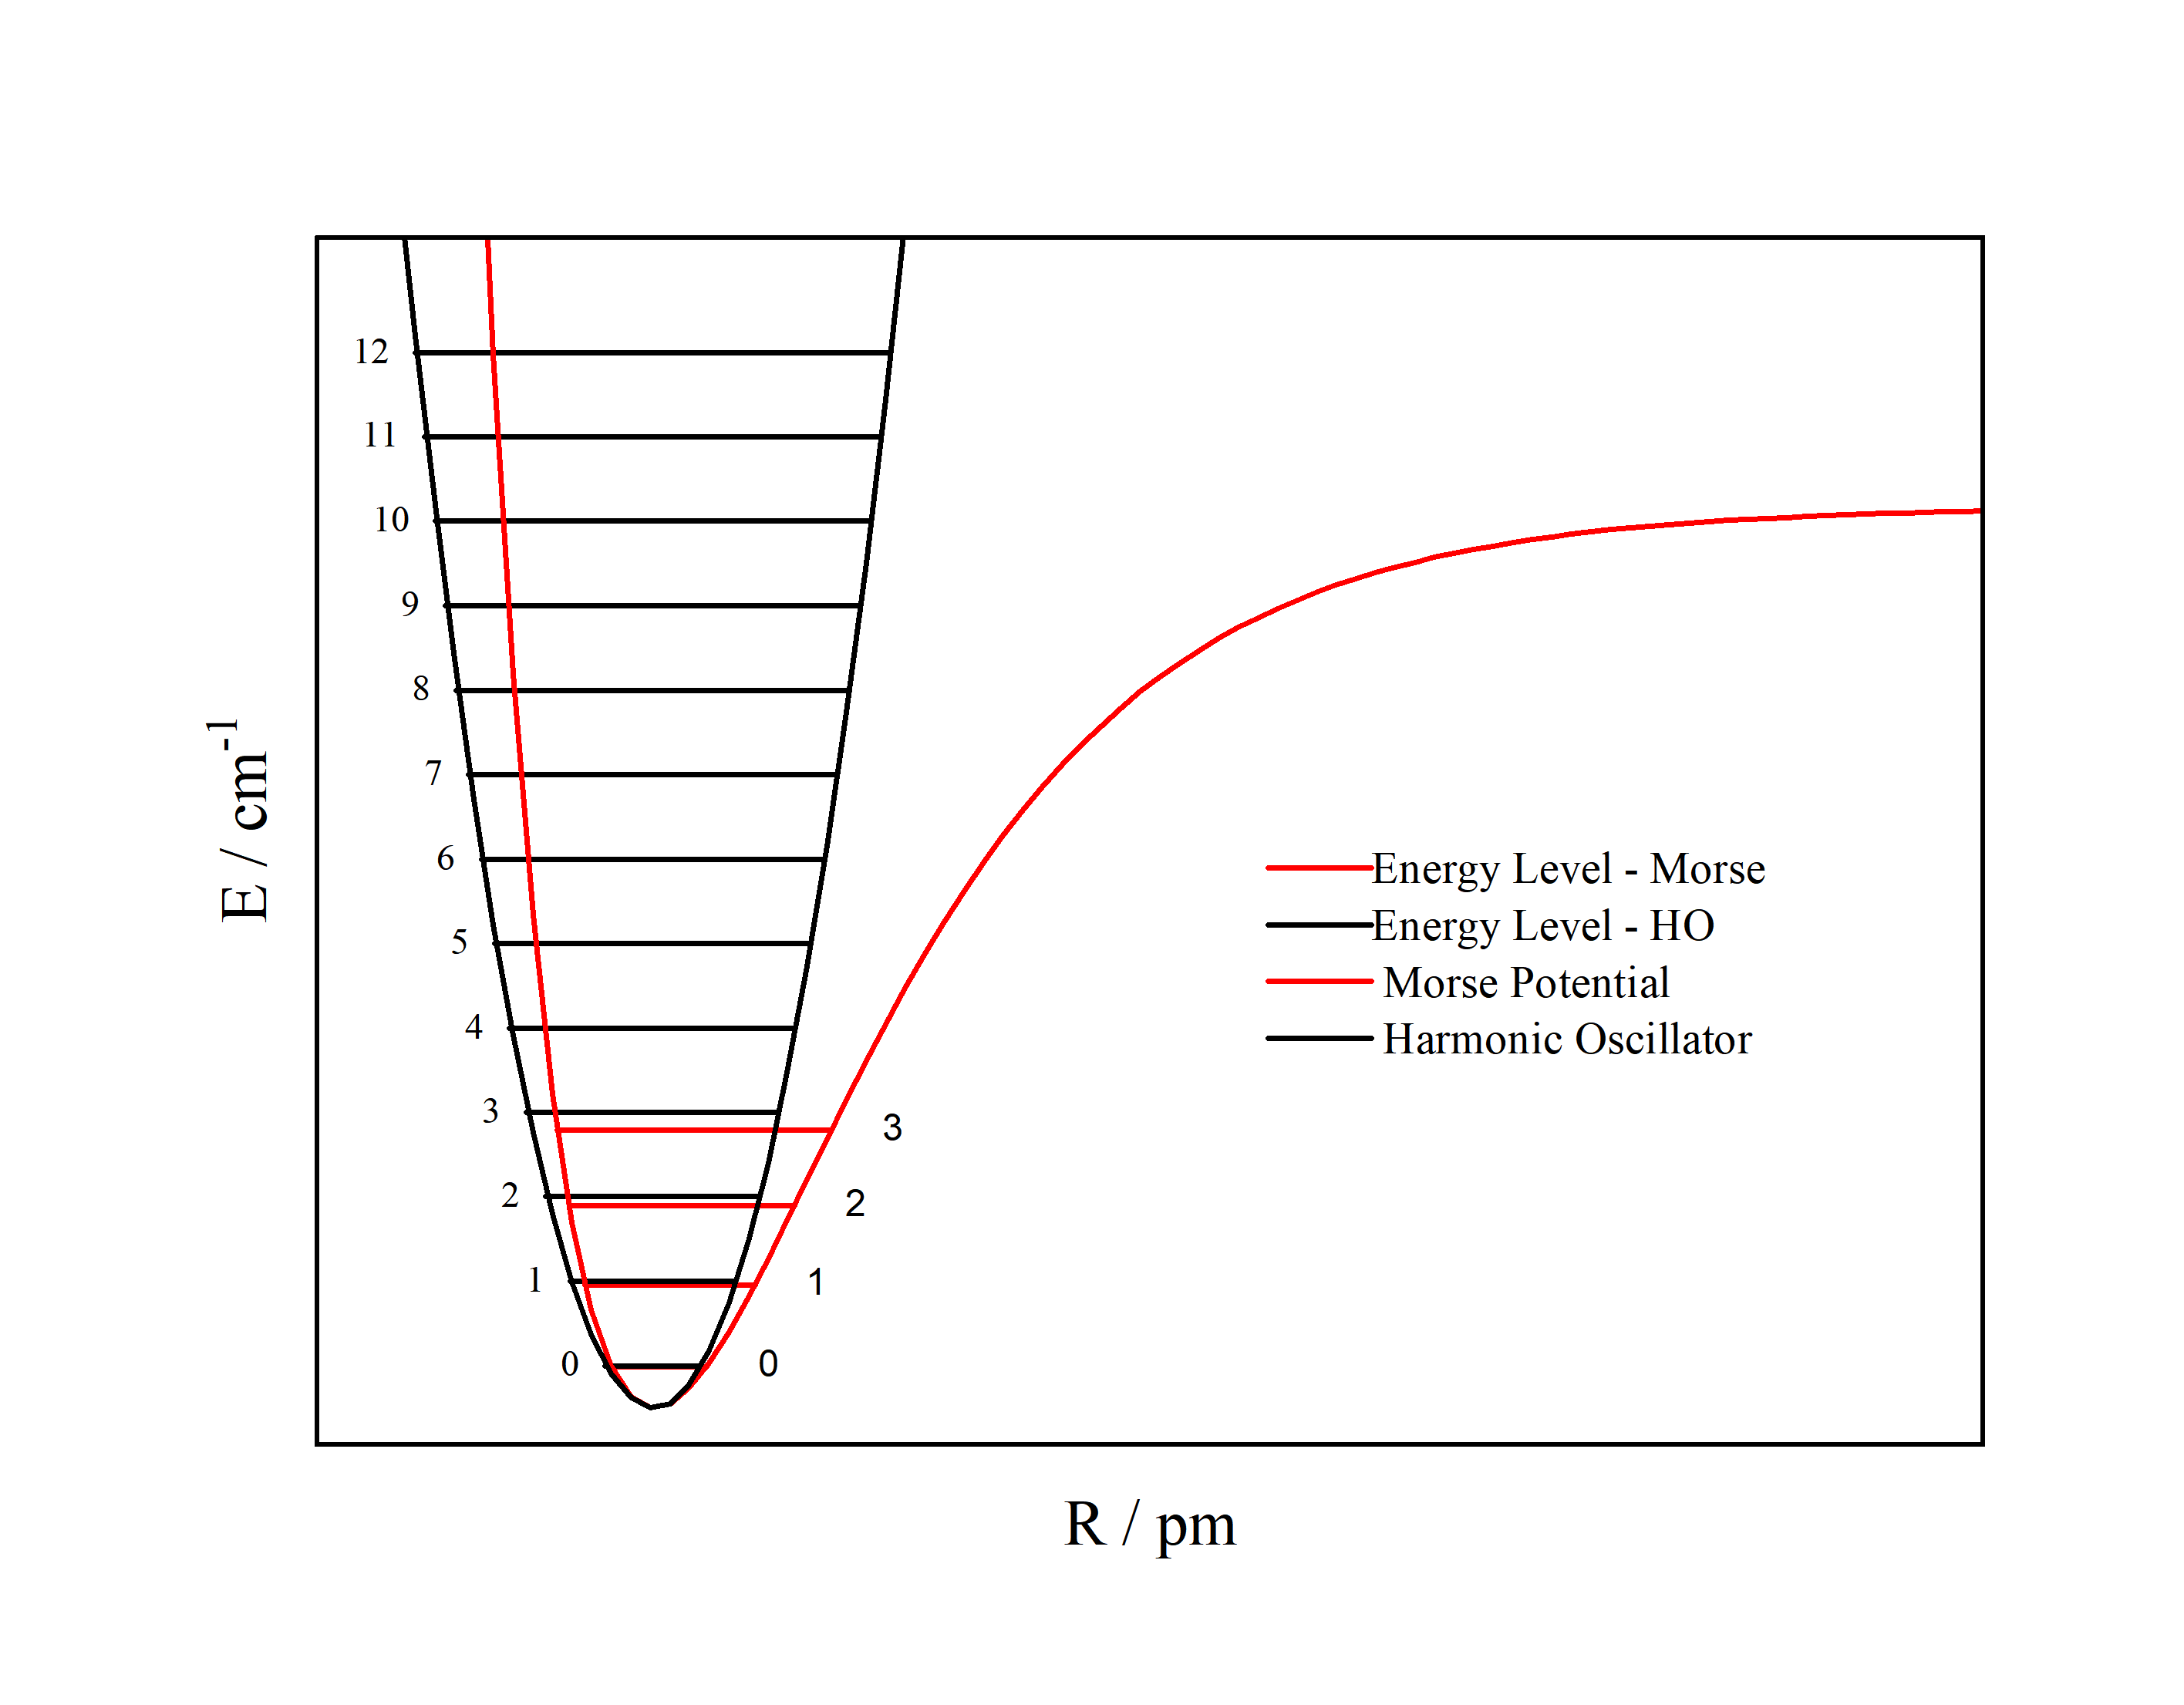
\includegraphics{Figures/Misc/QHA/MorsePotential.png}
    \captionsetup{font = footnotesize, justification = centering}
    \caption[The Harmonic Oscillator and Morse Potential]{A diagram showing the vibrational energy levels of a covalent bond modelled as a harmonic oscillator and with a Morse potential. For the harmonic oscillator, the vibrational energy levels are evenly spaced and continue to infinity. When modelled with a Morse potential, the separation between energy levels gradually converges to 0 at which point the bond will dissociate.}
    \label{fig:SHO_morse}
\end{figure}

As described in \Cref{subsec:vibmodestheory}, the energy of the system is obtained through a Taylor expansion with respect to the displacement of the nuclei from their equilibrium positions, given by:

\begin{equation}
\boldsymbol{E} = \boldsymbol{E}_0 + \frac{\delta \boldsymbol{E}}{\delta u}.u + \frac{1}{2!} \frac{\delta^2 \boldsymbol{E}}{\delta u^2}.u^2 + \frac{1}{3!} \frac{\delta^3 \boldsymbol{E}}{\delta u^3}.u^3 + ...
\label{eqn:ETaylor2}
\end{equation}

Only terms up to the term which is proportional to \(x^2\) are usually included as this allows calculation of the dynamical matrix. Whilst this is sufficient for approximately harmonic systems, the lack of inclusion of higher order terms removes both the inclusion of anharmonicity into the mode itself and the mode coupling that arises as a result of mode anharmonicity, as the \acrshort{ho} model also does not incorporate interaction between modes. Without allowing for this, properties such as vibrational relaxation, phonon lifetimes and thermal conductivity will likely be incorrectly predicted. Currently, owing to the requirement of \acrshort{dft} for every ion to be in its ground electronic state, temperature is not incorporated which generally allows the harmonic approximation to be used. Incorporating higher order terms would allow for peak widths to be calculated from first principles rather than empirically matching to experiment. However, incorporating these higher order terms into the calculation requires using multiple unit cells which will drastically increase the computational resources required to the point of unfeasibility for large systems with complex bonding such as \acrshort{alm}, but has been demonstrated for less complicated systems \cite{Erba2019}. For isolated \acrshort{ho}s, the mode frequencies are not dependent on interatomic distances and the equilibrium volume of a crystal does not depend on temperature. It is known that thermal expansion occurs in nearly all systems which manifests in a temperature dependence of equilibrium bond lengths and \acrshort{alm} also follows this trend \cite{Smith2005, Schreyer2014}. 

\subsection{Terahertz Time-Domain Spectroscopy with Variable Temperature}
The \acrshort{thz} absorption spectra of \acrshort{alm} between 4 and \SI{300}{K} are shown in \Cref{fig:alm_abs_co_temp}. This was accomplished by taking a spectrum at \SI{300}{K} and then cooling the sample to \SI{4}{K} where a spectrum was taken. The sample was then allowed to warm up and subsequent spectra were taken at each \SI{50}{K} step, culminating in a final spectrum taken at \SI{300}{K} where the best of the two was selected.

\begin{figure}[t]
\centering
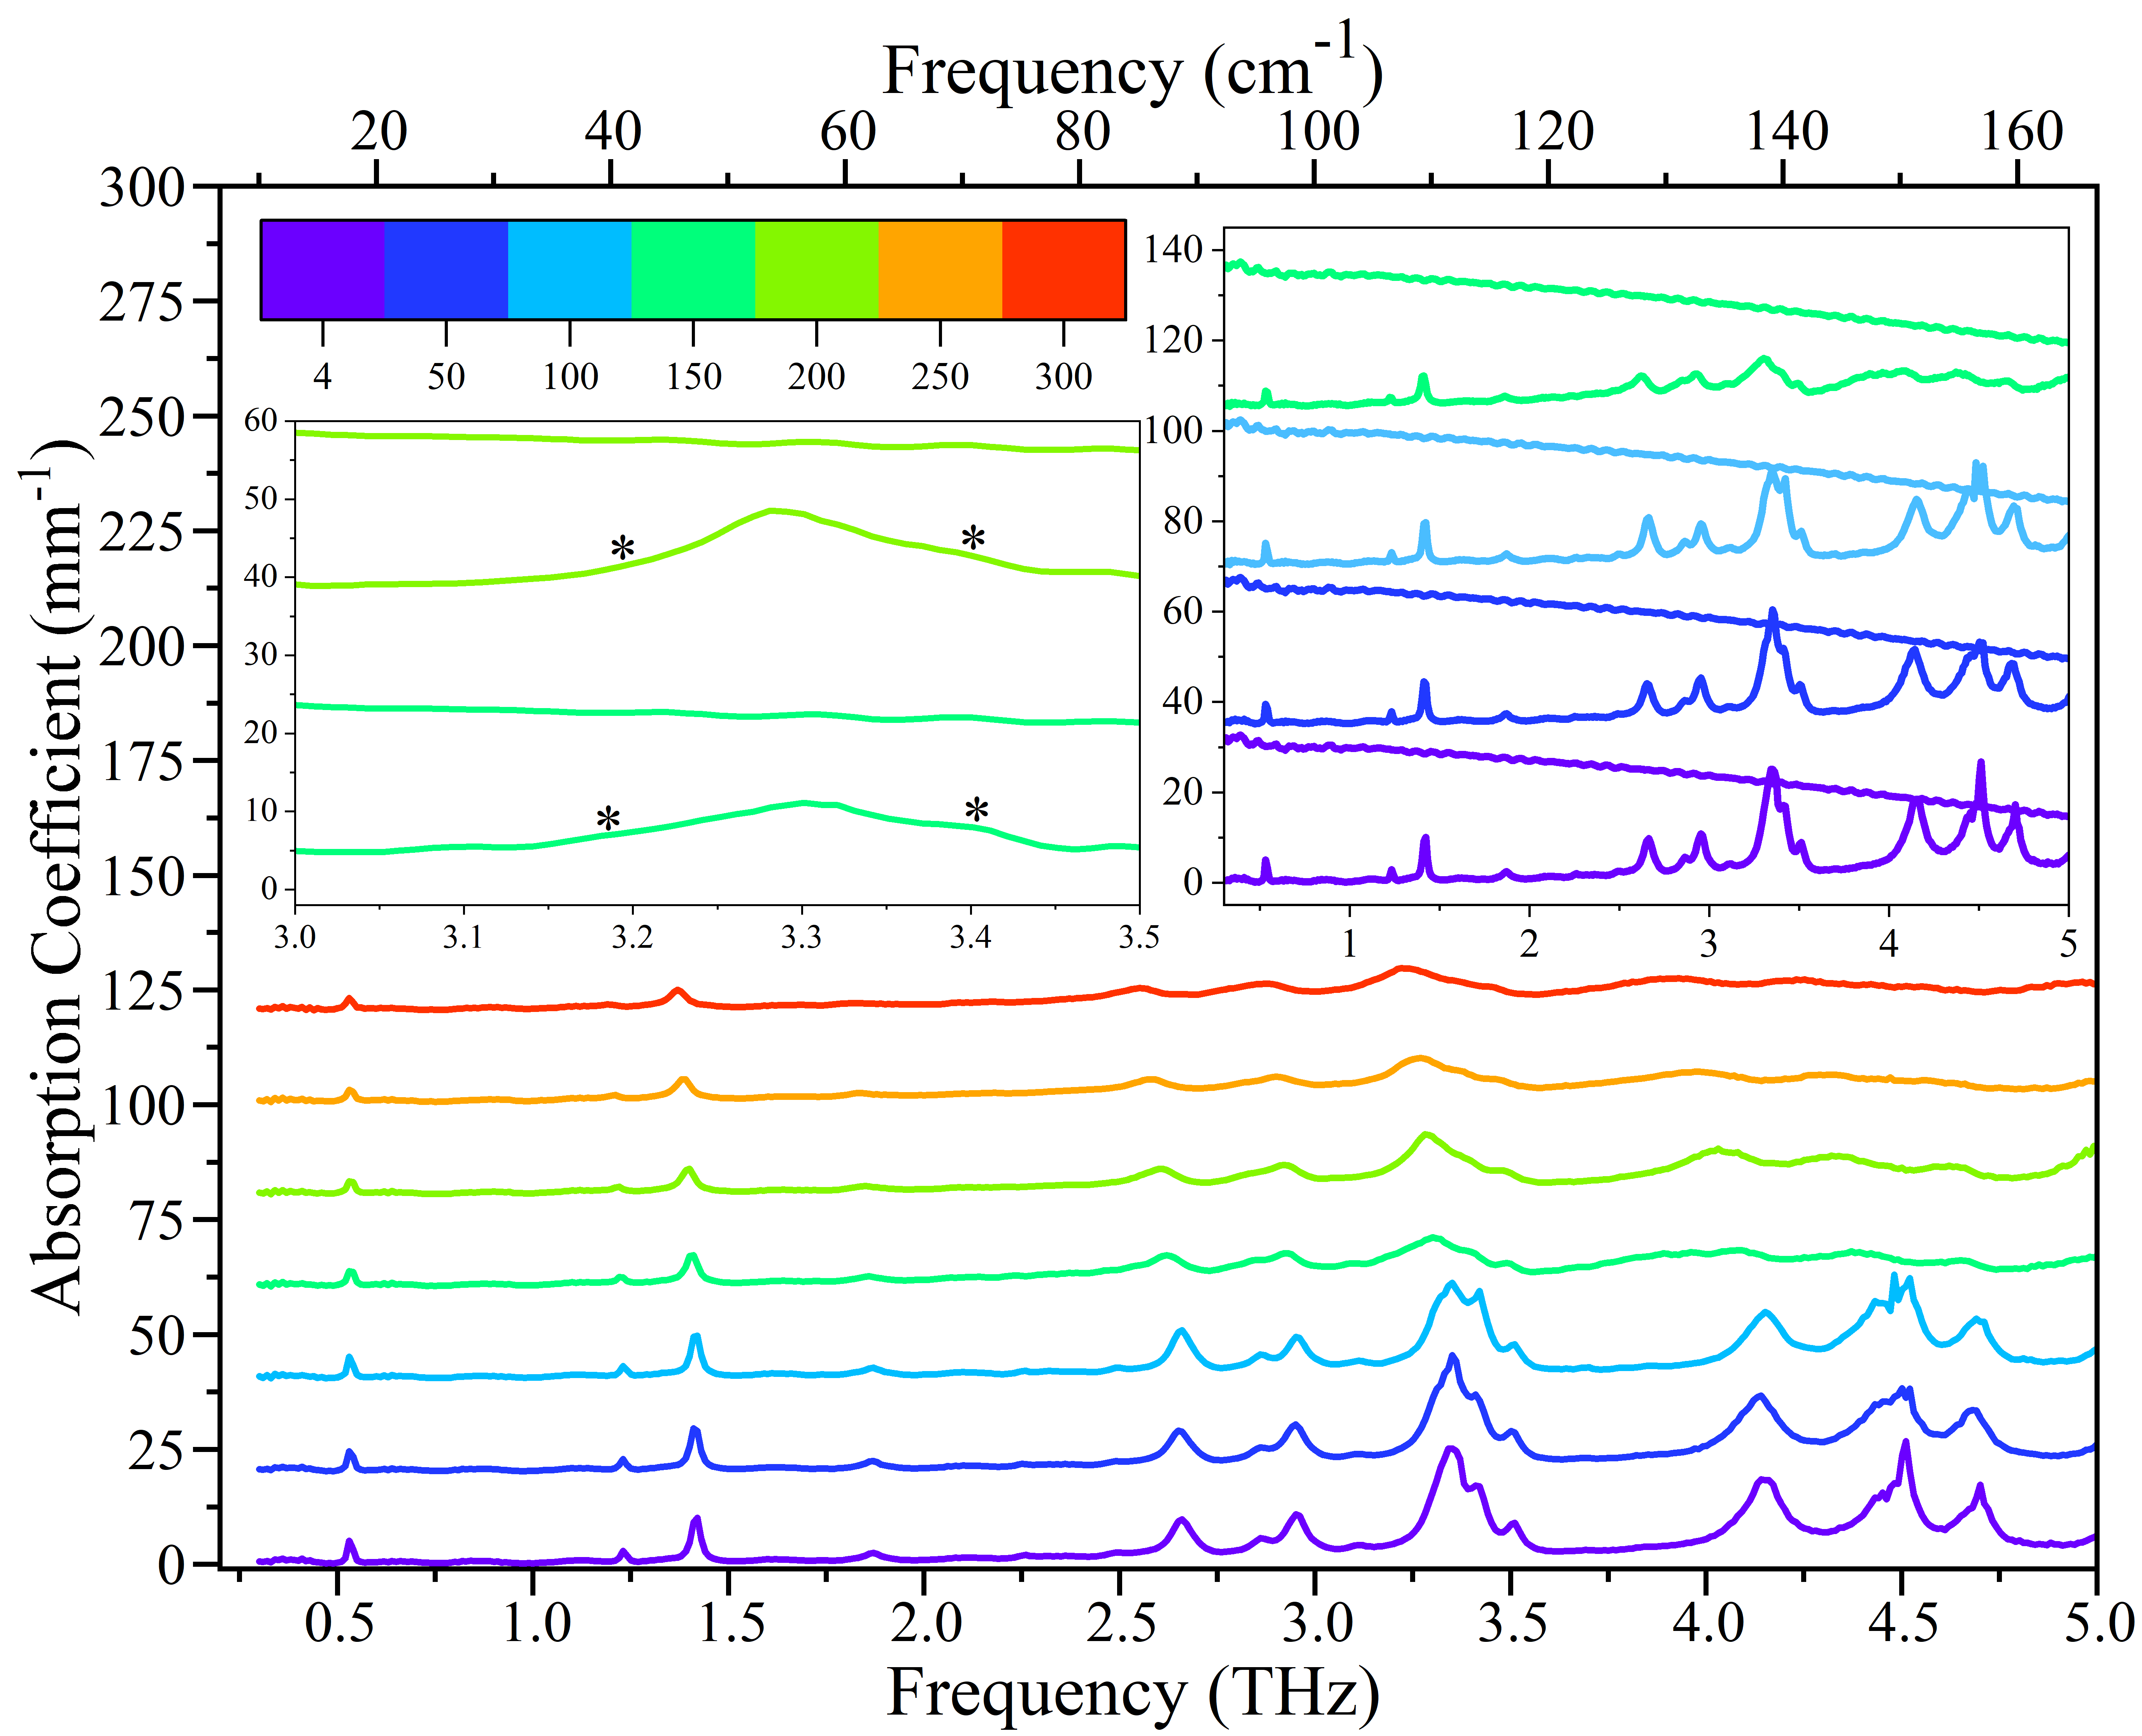
\includegraphics[scale=0.5]{Figures/Spectra/AbsCo10Offset.png}
\captionsetup{font = footnotesize}%, justification = centering}
\caption[The Terahertz Absorption Spectra of \(\alpha\)-Lactose Monohydrate between 4 and \SI{300}{K}]{Main - The terahertz absorption spectra of \(\alpha\)-Lactose Monohydrate between 4 and \SI{300}{k} with spectra being measured in \SI{50}{K} steps. Each measurement has been offset by \SI{20}{cm^{-1}} for clarity.
\vspace{1mm}

Left Inset - The absorption and maximum absorption for the 150 and \SI{200}{K} measurements. Whilst it is expected that the main peak will decrease in height with increasing temperature, it is proposed that peak broadening of the starred peaks contributes to an increase in peak height for the \SI{200}{K} measurement. 
\vspace{1mm}

Right Inset - The absorption and maximum absorption for the 4 to \SI{150}{K} measurements. Owing to the absorption maximum being crossed by multiple peaks, the \SI{150}{K} measurement is the first measurement that can be considered completely accurate.}
\label{fig:alm_abs_co_temp}
\end{figure}

The spectra change significantly as temperature is increased, which is mostly the result of homogeneous peak broadening owing to increased thermal motion across the entire spectrum. This is a result of thermal broadening and is common for \acrshort{thz} absorption spectra. Additionally, at \SI{10}{K} only the first vibrational energy level will be populated but at \SI{300}{K}, \(k_BT\) is approximately equal to \SI{6.1}{\acrshort{thz}} so multiple energy levels will be populated which leads to further peak broadening. The peak positions themselves tend to shift to lower frequencies for all peaks with the exception of the first peak, and this is shown in \Cref{fig:exppeakshifts}. The five modes shown are indicated in \Cref{fig:starredpeaks} with an asterisk, and these peaks have been chosen owing to their visibility throughout the temperature range in question. These five peaks will be referred to as Mode 1 to Mode 5 respectively from now on, for brevity. This red\nobreakdash-shifting of the mode frequency is a common trend for modes in the \acrshort{thz} frequency range \cite{Allen2021} and is believed to arise from the anharmonicity of a given mode, with some exceptions where the peak will shift to a higher frequency \cite{Walther2003}. The stability of the first mode with temperature may demonstrate the harmonic nature of this mode. Finally, it can be seen that above \SI{150}{K} the peak heights drastically drop and comparison becomes more challenging. For this reason, all subsequent analysis will be performed on data up to \SI{3.5}{\acrshort{thz}}. It should be noted that only the peak heights for \SI{150}{K} and above can be considered accurate as the maximum absorption value is reached below this temperature. The increase in peak height between 150 and \SI{200}{K} is believed to be owing to thermal broadening as indicated by the left inset in \Cref{fig:alm_abs_co_temp}.

\begin{figure}[ht!]
\centering
\begin{subfigure}{1\textwidth}
\centering
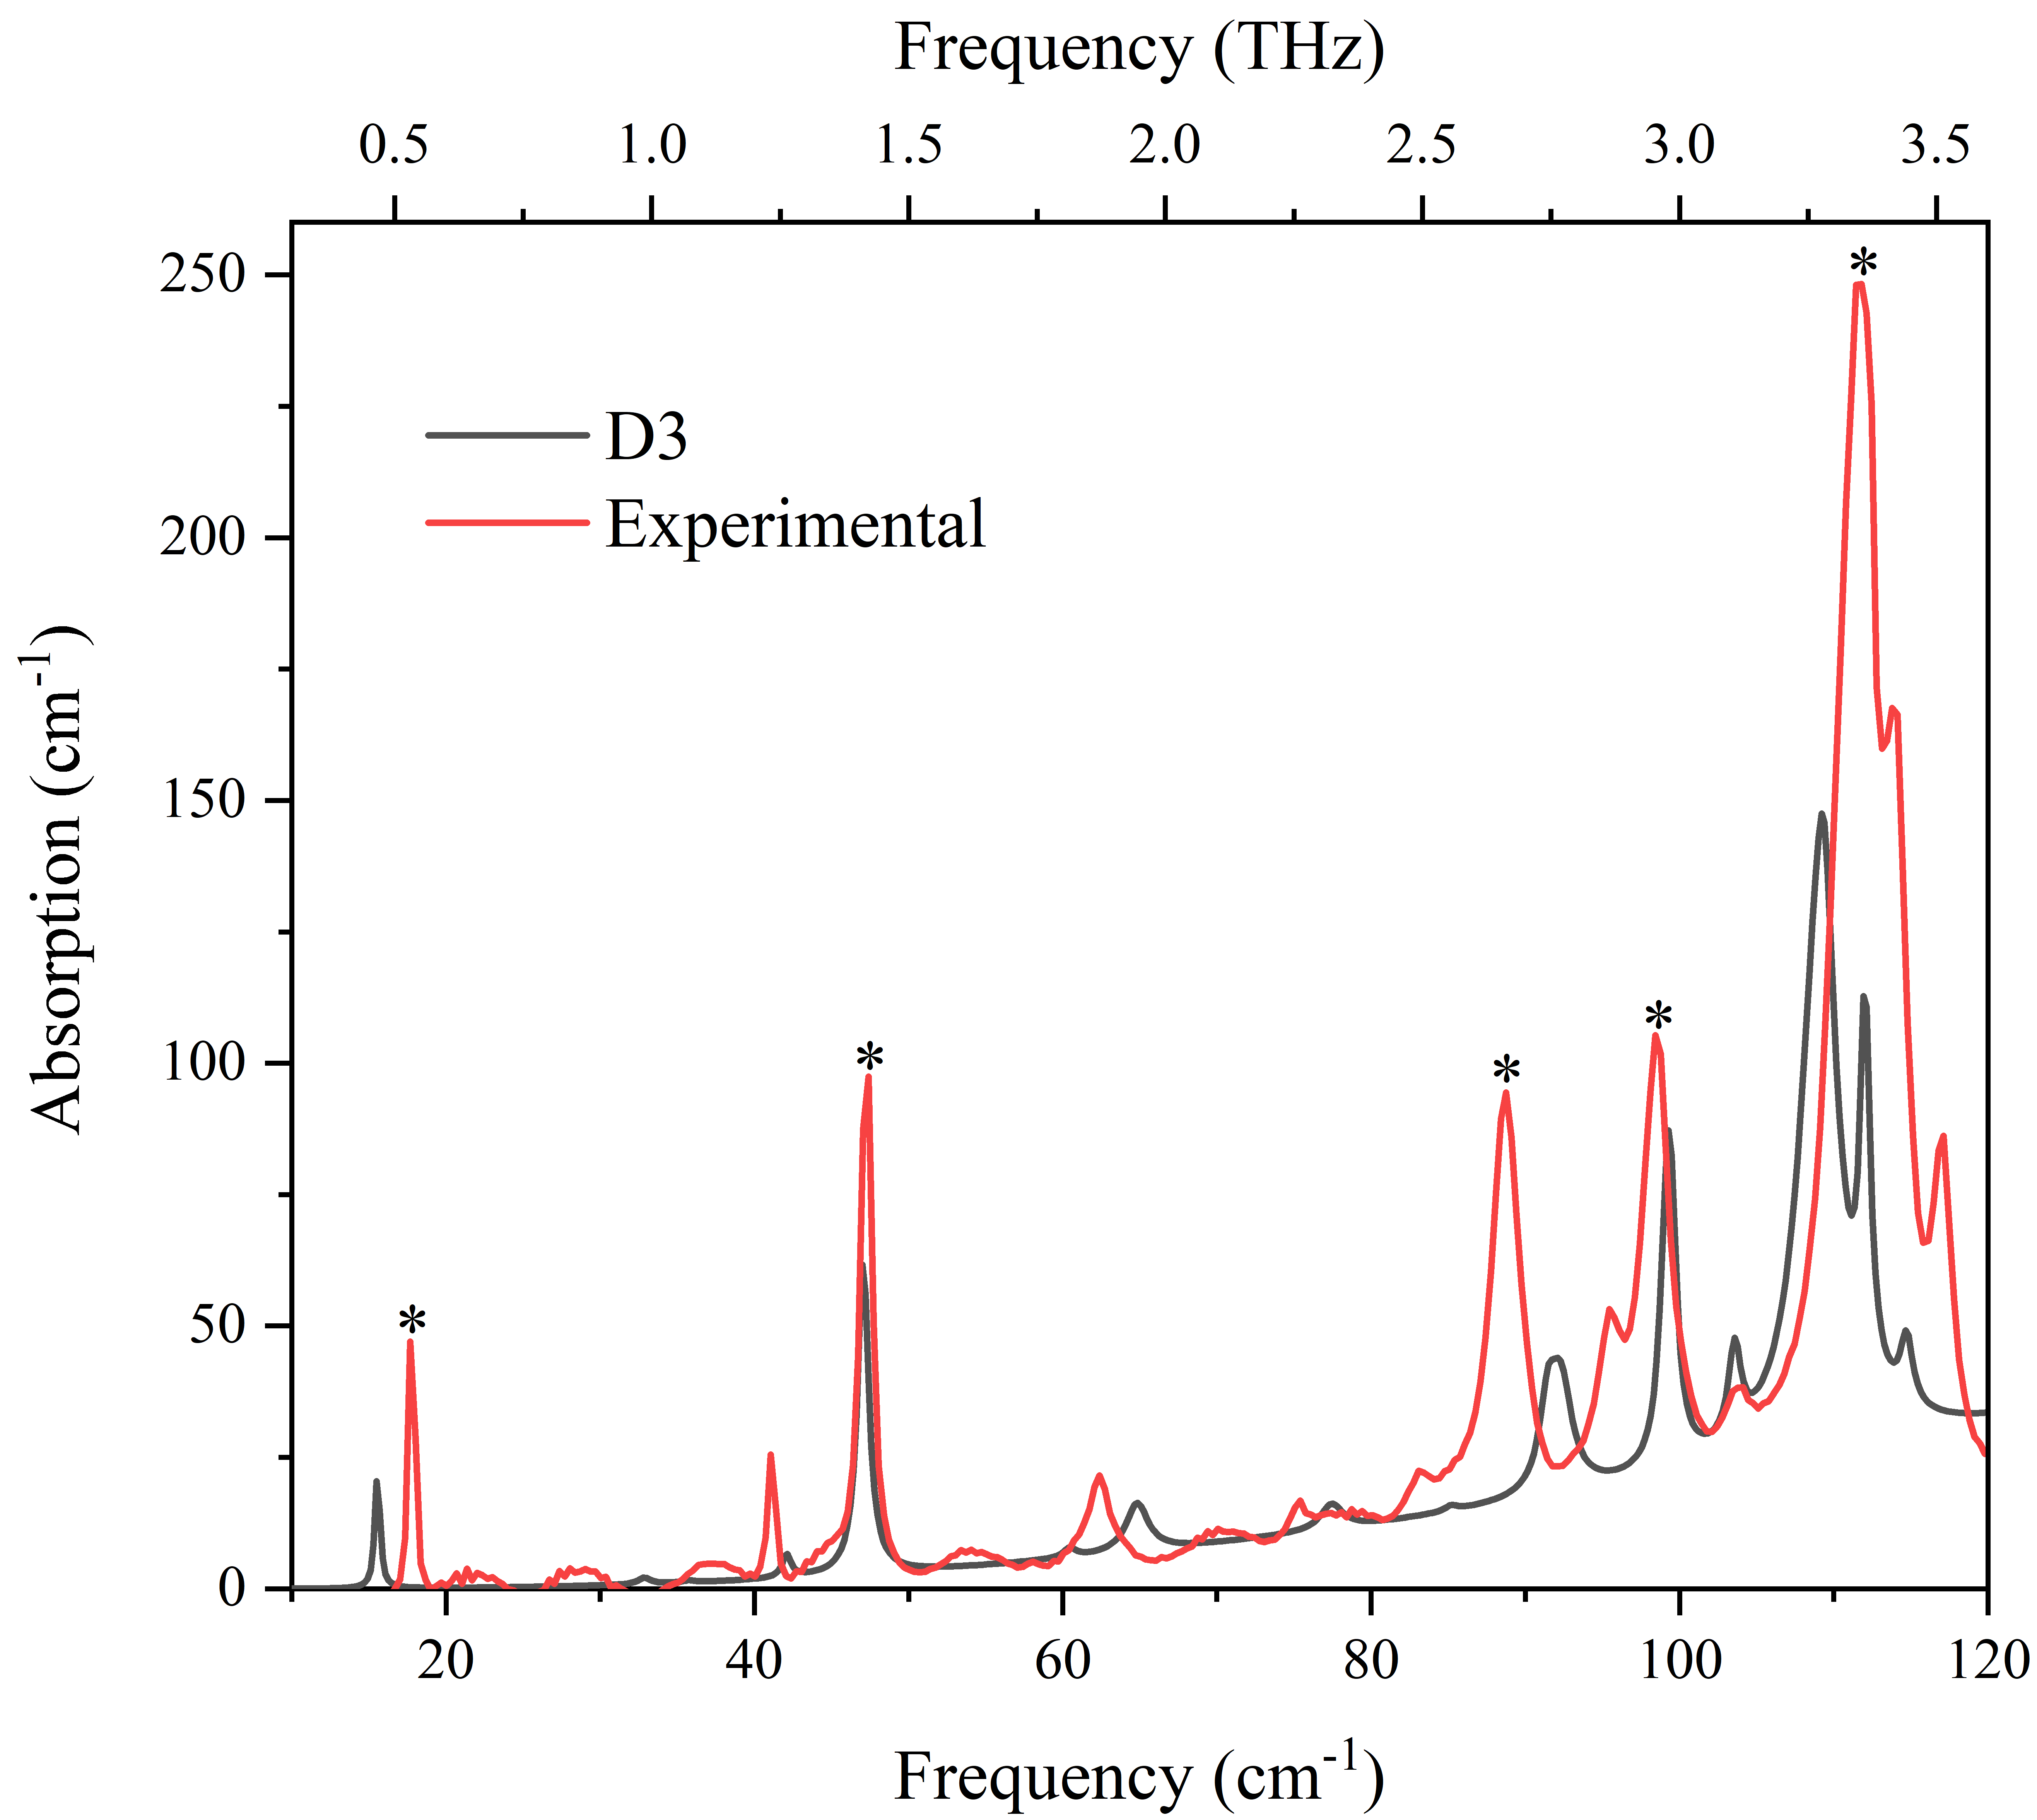
\includegraphics[scale=0.5]{Figures/Spectra/D3ExpDiffG.png}
\caption{The calculated terahertz absorption spectrum using the harmonic approximation. The starred peaks are the modes selected for further investigation.}
\label{fig:starredpeaks}
\end{subfigure}

\begin{subfigure}{1\textwidth}
\centering
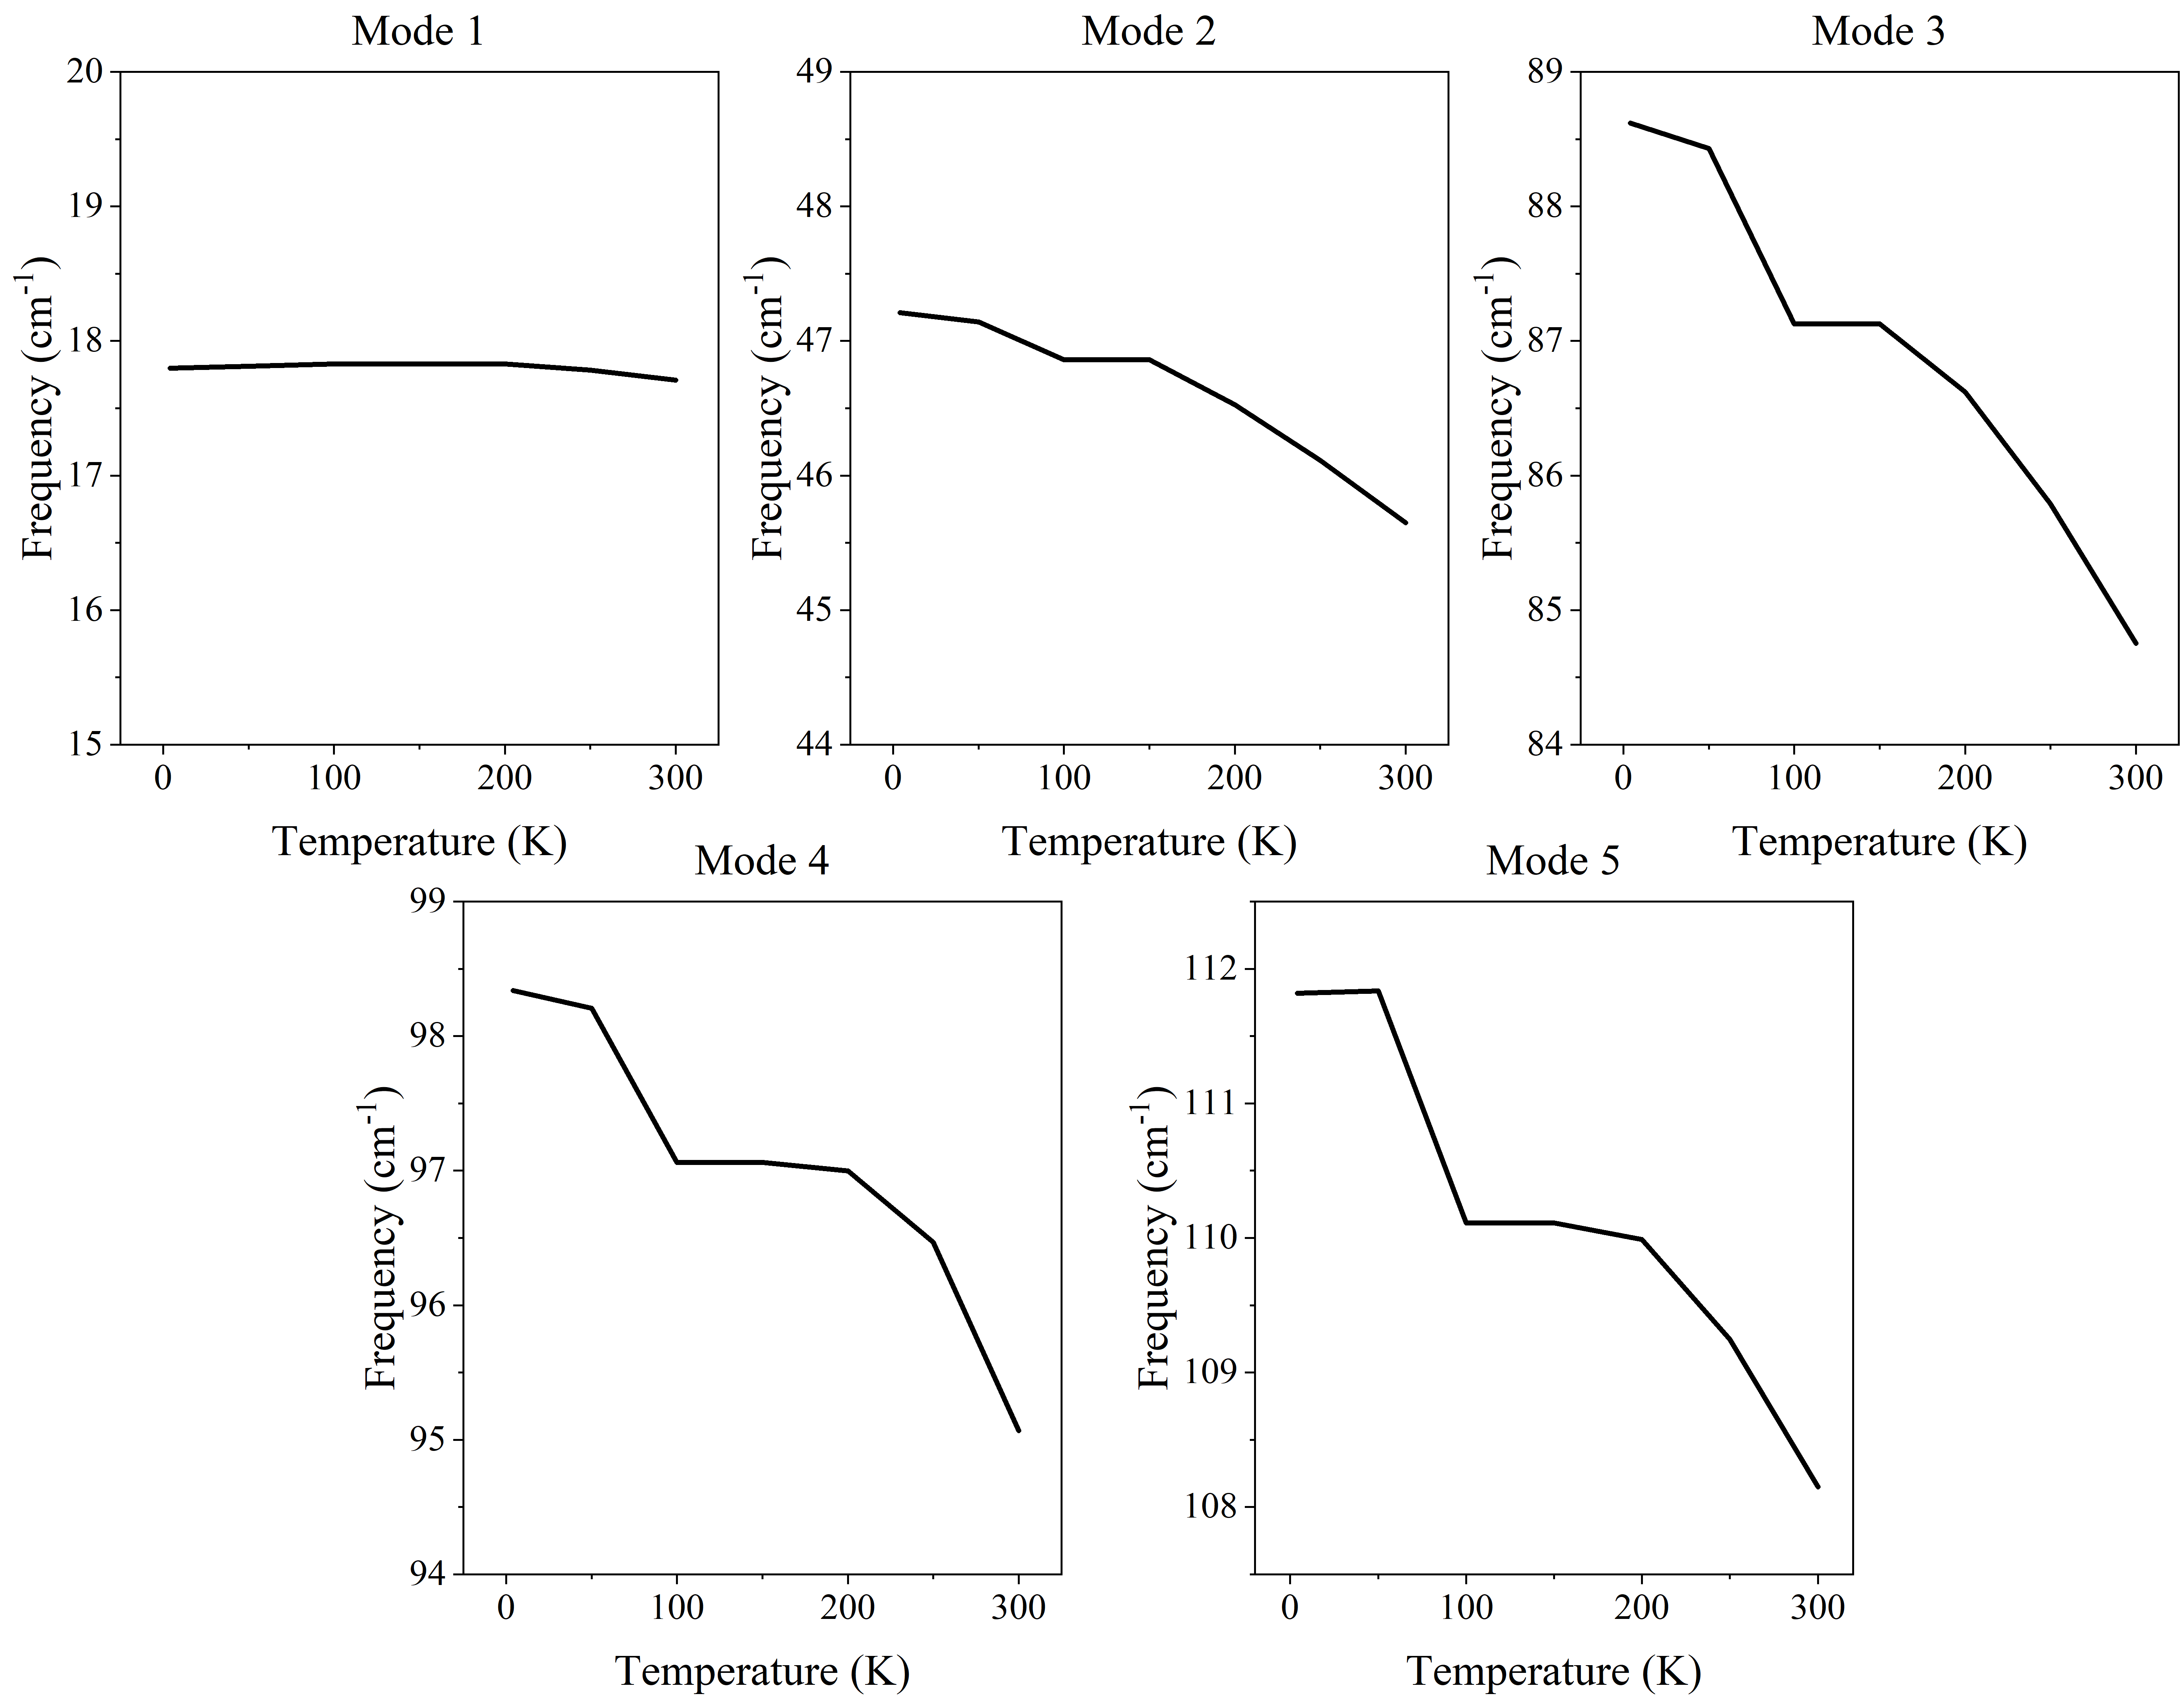
\includegraphics[scale=0.5]{Figures/Misc/QHA/ExpWidthsG.png}
\caption{Experimental peak widths as a function of temperature for the starred peaks shown above.}
\label{fig:exppeakshifts}
\end{subfigure}

\captionsetup{font = footnotesize, justification = centering}
\caption[The Terahertz Absorption Spectrum using the Harmonic Approximation and the Temperature Dependence of the Experimental Peak Widths]{The terahertz absorption spectrum using the harmonic approximation and the temperature dependence of the experimental peak widths.}
\label{Fig:d3_exp_mode_temp}
\end{figure}

An additional benefit of incorporating anharmonicity allows prediction of the spectrum with temperature effects included. This can reduce the need to take experimental spectra at \SI{4}{K} which significantly complicates the process. Reaching these temperatures requires liquid He which is costly, hazardous and increases the complexity of the experimental apparatus required. It would be beneficial to not have to use any cooling methods and perform the same degree of analysis on a spectrum taken at room temperature. Whilst the anharmonic terms of the Taylor expansion of the energy of the system is an extremely computationally costly method of understanding the full energy landscape, there are other methods that can be used to understand the effect of temperature and anharmonicity on systems. One of the most prevalent of these is molecular dynamics (\acrshort{md}) simulations.

\subsection{Molecular Dynamics}
\acrshort{md} simulations are a class of computational simulations that model the movement of particles, which can be atoms or entire molecules \cite{Fermi1955}. If the forces between particles can be calculated, this can be turned into a trajectory that the particle will move along within a given time step. This allows the dynamical behavior of a system to be studied as long as the potentials between particles is correctly modelled and the time step is similar to the time scale of the phenomena being studied. Vibrational motion can be considered to be a collection of atoms or molecules moving along repeated trajectories and so is appropriate for study by \acrshort{md}. 

Temperature can be calculated using both the kinetic temperature, where the temperature is a function of the total kinetic energy of the constituent particles and the canonical probability distribution function which uses the Boltzmann distribution \cite{Sri2021}. This allows temperature to be controlled using a thermostat, which is simply an algorithm that prevents the system from leaving thermal equilibrium. There are many different variations of this algorithm, including the Nose\nobreakdash-Hoover thermostat \cite{Braka2003} and the Braga\nobreakdash-Travis thermostat \cite{Patra2014} but all suffer from some form of limitation. These has been used for predicting THz absorbance spectra \cite{Dai2020} but this was most successful for spectra taken at temperatures close to \SI{0}{K}. 

One of the most significant challenges of this type of simulation is modelling the inter\nobreakdash-particle potentials correctly and has led to the development of several sub\nobreakdash-categories of \acrshort{md}. If these potentials are incorrectly modelled then any vibrational data that can be extracted will not be accurate. Traditionally, these were derived from empirical data extracted from the experimental spectra \cite{Thakur1998, Haas1995, Miller2004} but can also be constructed through first principles methods  \cite{Wang2020}. One method that has shown much success is \textit{ab\nobreakdash-initio} \acrshort{md} \cite{Car2005} which uses first\nobreakdash-principles methods such as \acrshort{dft} to calculate the inter\nobreakdash-particle potentials \cite{Gai1998}. By repeating the simulation multiple times, the statistical distribution of the possible evolutions of a system can be measured. \acrshort{md} simulations are able to explore the potential energy surface without the limitations of the harmonic approximation but the nature of the mode can be challenging to determine, limiting their overall utility for interpreting experimental vibrational spectra. Whilst anharmonic properties of the mode such as phonon lifetime and coupling can be determined, this is prohibitively expensive for complex organic systems such as \acrshort{alm} and so has not been attempted in this work.

\section{The Quasi-Harmonic Approximation}
 Some degree of the anharmonic behaviour of a system can also be calculated using another method, which is by using the the Quasi\nobreakdash-Harmonic Approximation (\acrshort{qha}). Phenomena such as thermal expansion cannot be reproduced using the harmonic approximation owing to the frequency of each mode being independent of temperature \cite{yatsyshyn2015handbook}. This method is based on the assumption that the harmonic nature of vibrational motion is valid for all values of a given lattice constant which controls the volume of a crystalline system's unit cell. This allows the volume of a system to behave as a proxy for temperature and the thermodynamical properties dependent on temperature can be extracted. Through this, the harmonic approximation that underpins most vibrational calculations holds true for each volume whilst the increased volume as temperature increases can be accounted for. 

Using \acrshort{dft} with the method described in \Cref{subsec:GODMCalc}, implemented using the VASP package for the optimisation of atomic positions and the dynamical matrix was calculated using Phonopy with VASP as the computational engine. Five unit cells were generated with volumes between 766.47\nobreakdash--\SI{781.57}{\angstrom}, with differences of approximately \SI{3.8}{\angstrom^3} between them.  The volume and corresponding total energy of each cell is shown in \Cref{fig:ev}. \acrshort{alm} has a symmetry of \(P_{21}\) which must be conserved when expanding the unit cell. Initial cell choice ranges were 99\nobreakdash--104\% of the optimised unit cell volume. but this resulted in a volume\nobreakdash-temperature curve which did not overlap with the optimised unit cell volume at \SI{0}{K}. Smaller increments were then attempted with a range of 101.5\nobreakdash--103.5\% which were more successful. Five were chosen as this is the minimum number of volumes required but more would improve the accuracy of the calculations. However, owing to the size of the \acrshort{alm} unit cell this was decided to be prohibitively expensive in terms of computational resources.

\begin{figure}[h]
\centering
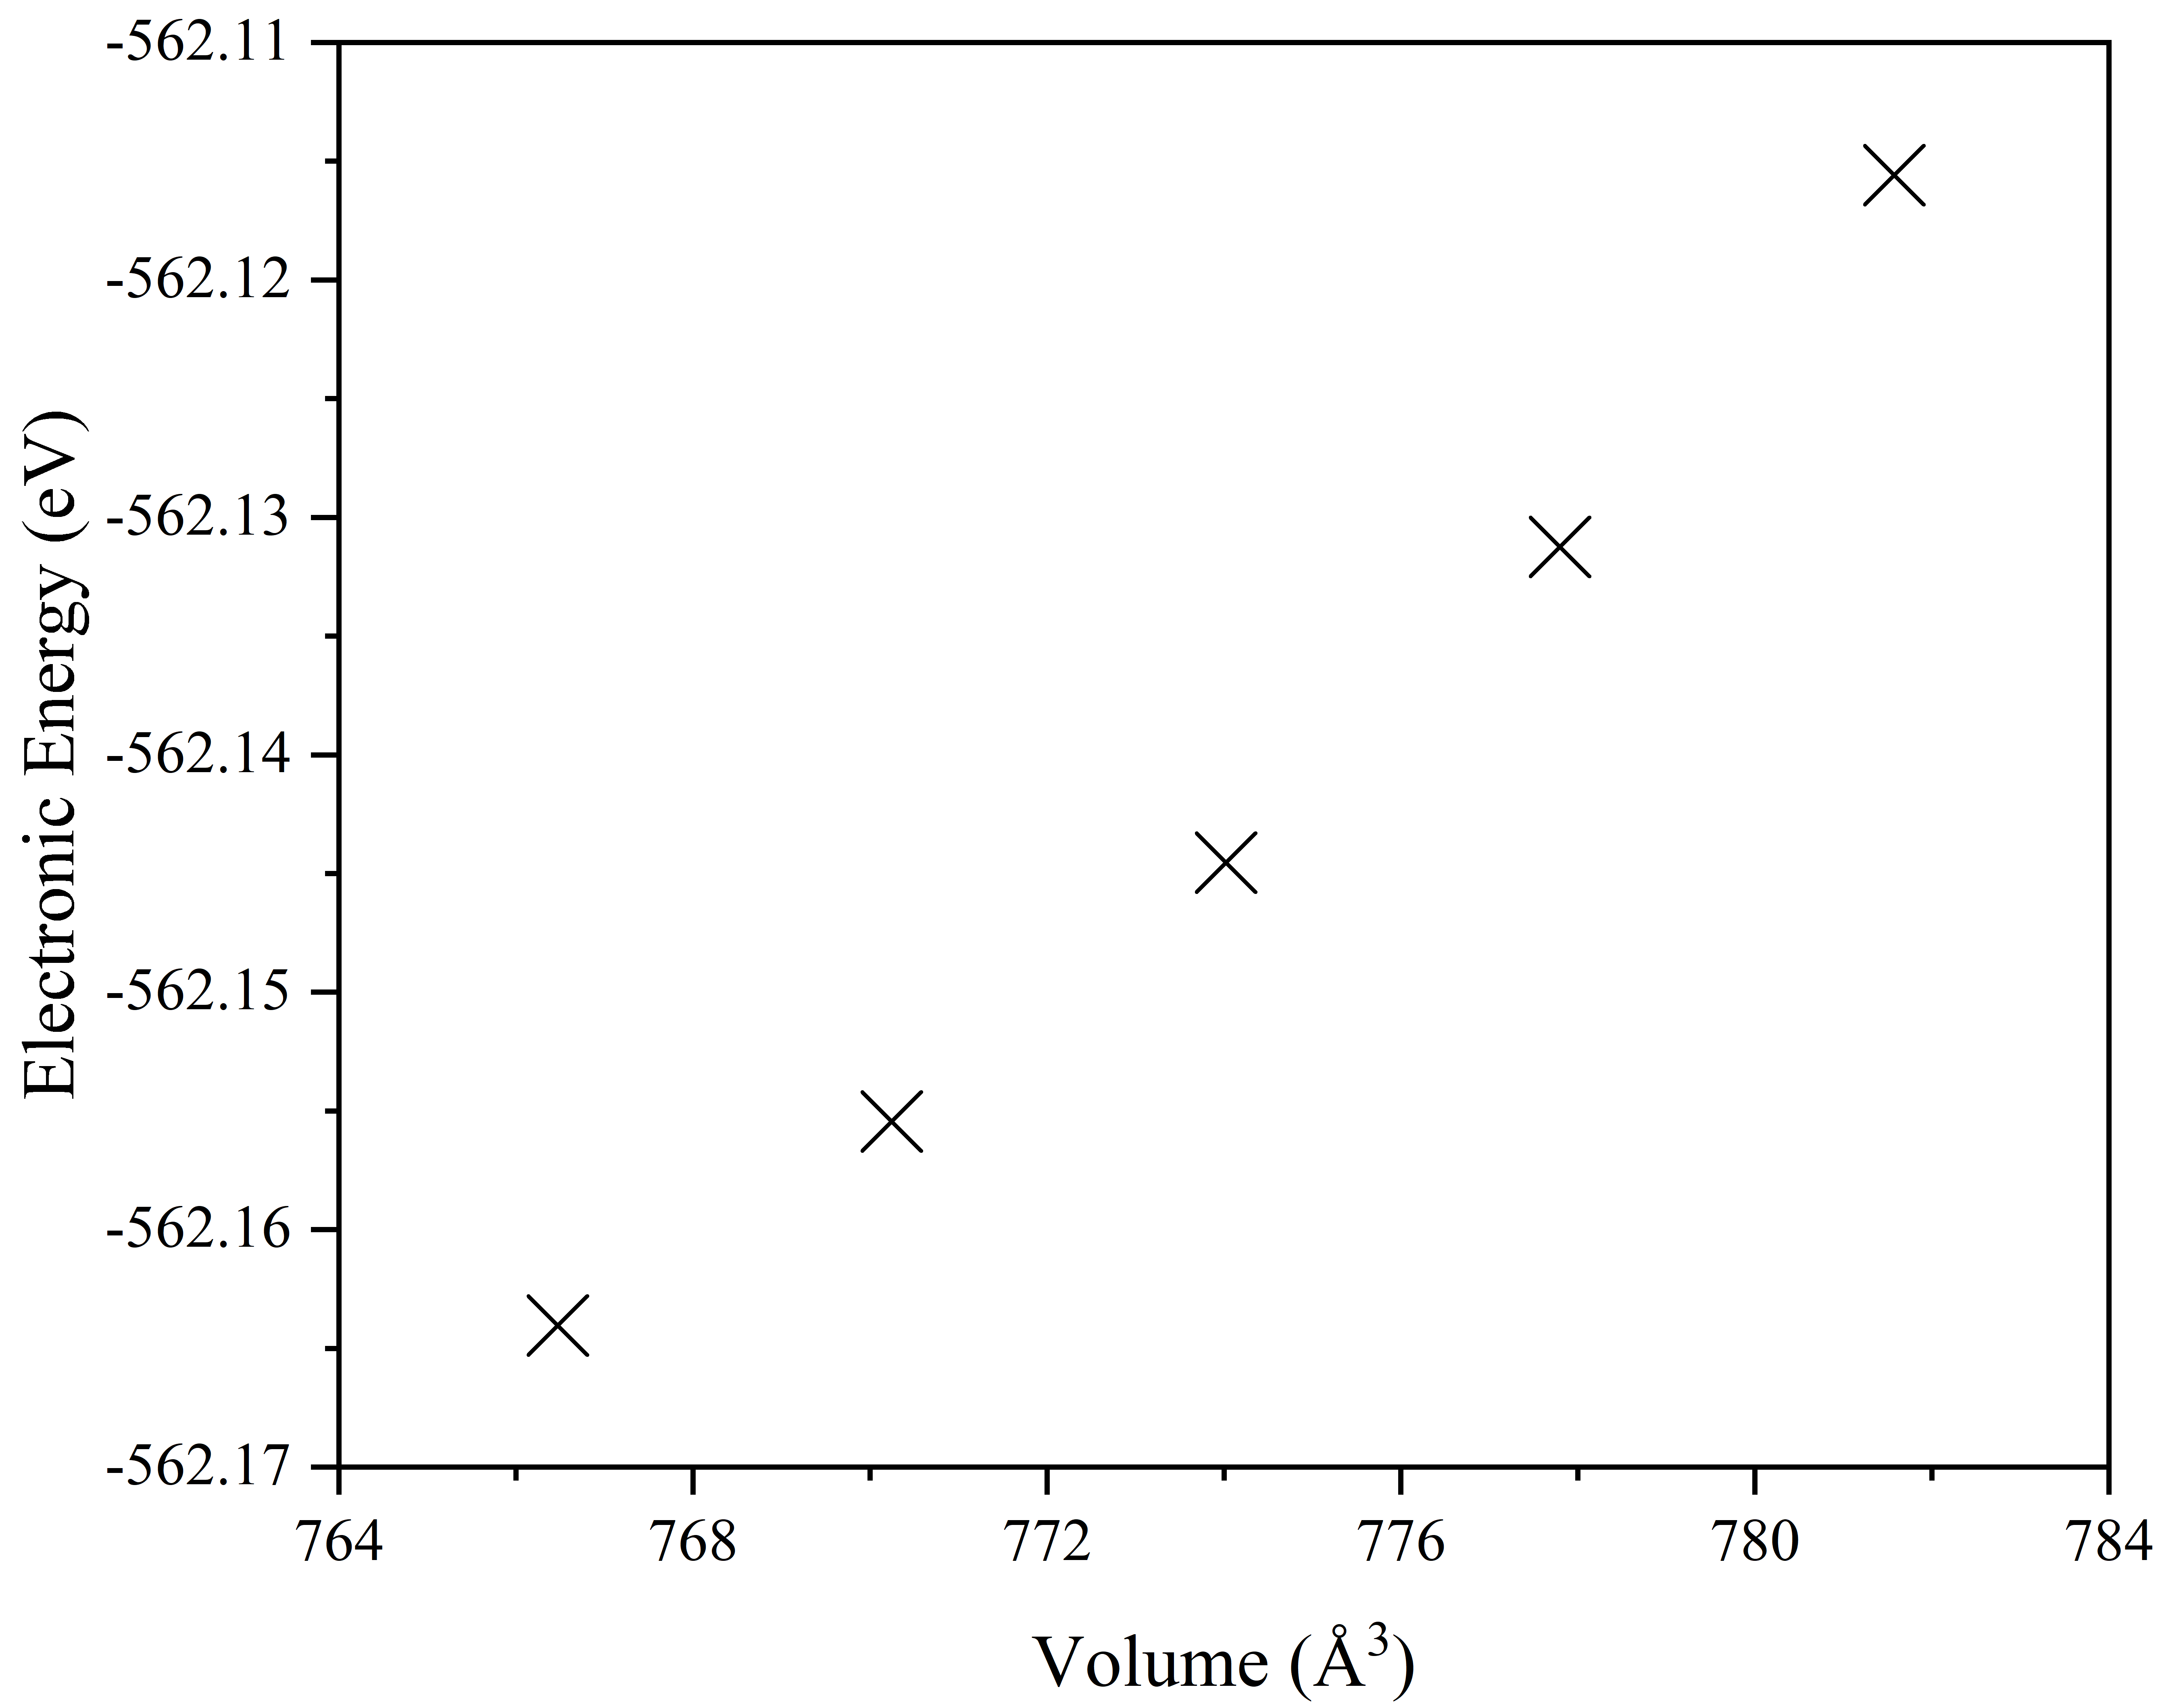
\includegraphics[width=0.6\textwidth]{Figures/Misc/QHA/evG.png}
\captionsetup{font = footnotesize, justification = centering}
\caption[The Selected Volumes and Corresponding Energies used for the Quasi-Harmonic Approximation]{The volumes and corresponding energies of the five unit cells used to calculate the thermal properties of the system under the quasi-harmonic approximation.}
\label{fig:ev}
\end{figure}

Whilst keeping the cell dimensions fixed, the atoms were allowed to relax to their lowest energy state and the dynamical matrix was calculated for each volume. The phonon frequencies were extracted and these are then used to derive the thermal properties for the system by using the relationship:

\begin{equation}
G_{T,p} = min[U(V) + F_{phonon}(T;V) + pV]
\label{eqn:qha_G}
\end{equation}


where \(G_{T,p}\) is the Gibbs free energy at constant temperature and pressure, \(U(V)\) is the total internal energy at constant volume\ \(p\) is the pressure, \(V\) is the unit cell volume and \(F_{phonon}(T;V)\) is the phonon Helmholtz free energy for a given temperature and volume. This is given by:

\begin{equation}
F_{phonon} = \frac{1}{2} \sum_{\textbf{q},\nu} \hbar\omega_{\textbf{q}} + k_BT \sum_{\textbf{q}} ln[1 - exp({\frac{-\hbar \omega_{\textbf{q}}}{k_BT}})]
\end{equation}

where \(\hbar\) is the reduced Planck constant, \(\omega_{\textbf{q},\nu}\) is the phonon frequency at wave vector \(\textbf{q}\) and \(k_B\) is the Boltzmann constant. By finding the minima of \Cref{eqn:qha_G} for each desired temperature, properties such as the thermal expansion of the system and heat capacity at constant pressure, \(C_p(T,p)\), can be calculated using these minima and thermodynamic relations such as:

\begin{equation}
C_p(T,p) = \left. -T\frac{\delta^2G(T,p)}{\delta T^2} = T\frac{\delta V(T,p)}{\delta T} \frac{\delta S(T;V)}{\delta V} \right\rvert_{V=V{T,p}}
\end{equation}

where \(V(T,p)\) is the equilibrium volume at \(T\) and \(p\).

\section{Analysis and Results}
\subsection{Thermal Expansion}
The relationship between volume and temperature is shown in \Cref{fig:tempvol} and its derivative, the thermal expansion coefficient, is shown in \Cref{fig:thermexp}. This gives unit cell volumes of 768.97 and \SI{771.86}{\angstrom^3} for 150 and \SI{300}{K} respectively. 

\begin{figure}[ht]
\centering

\begin{subfigure}{0.49\textwidth}
\centering
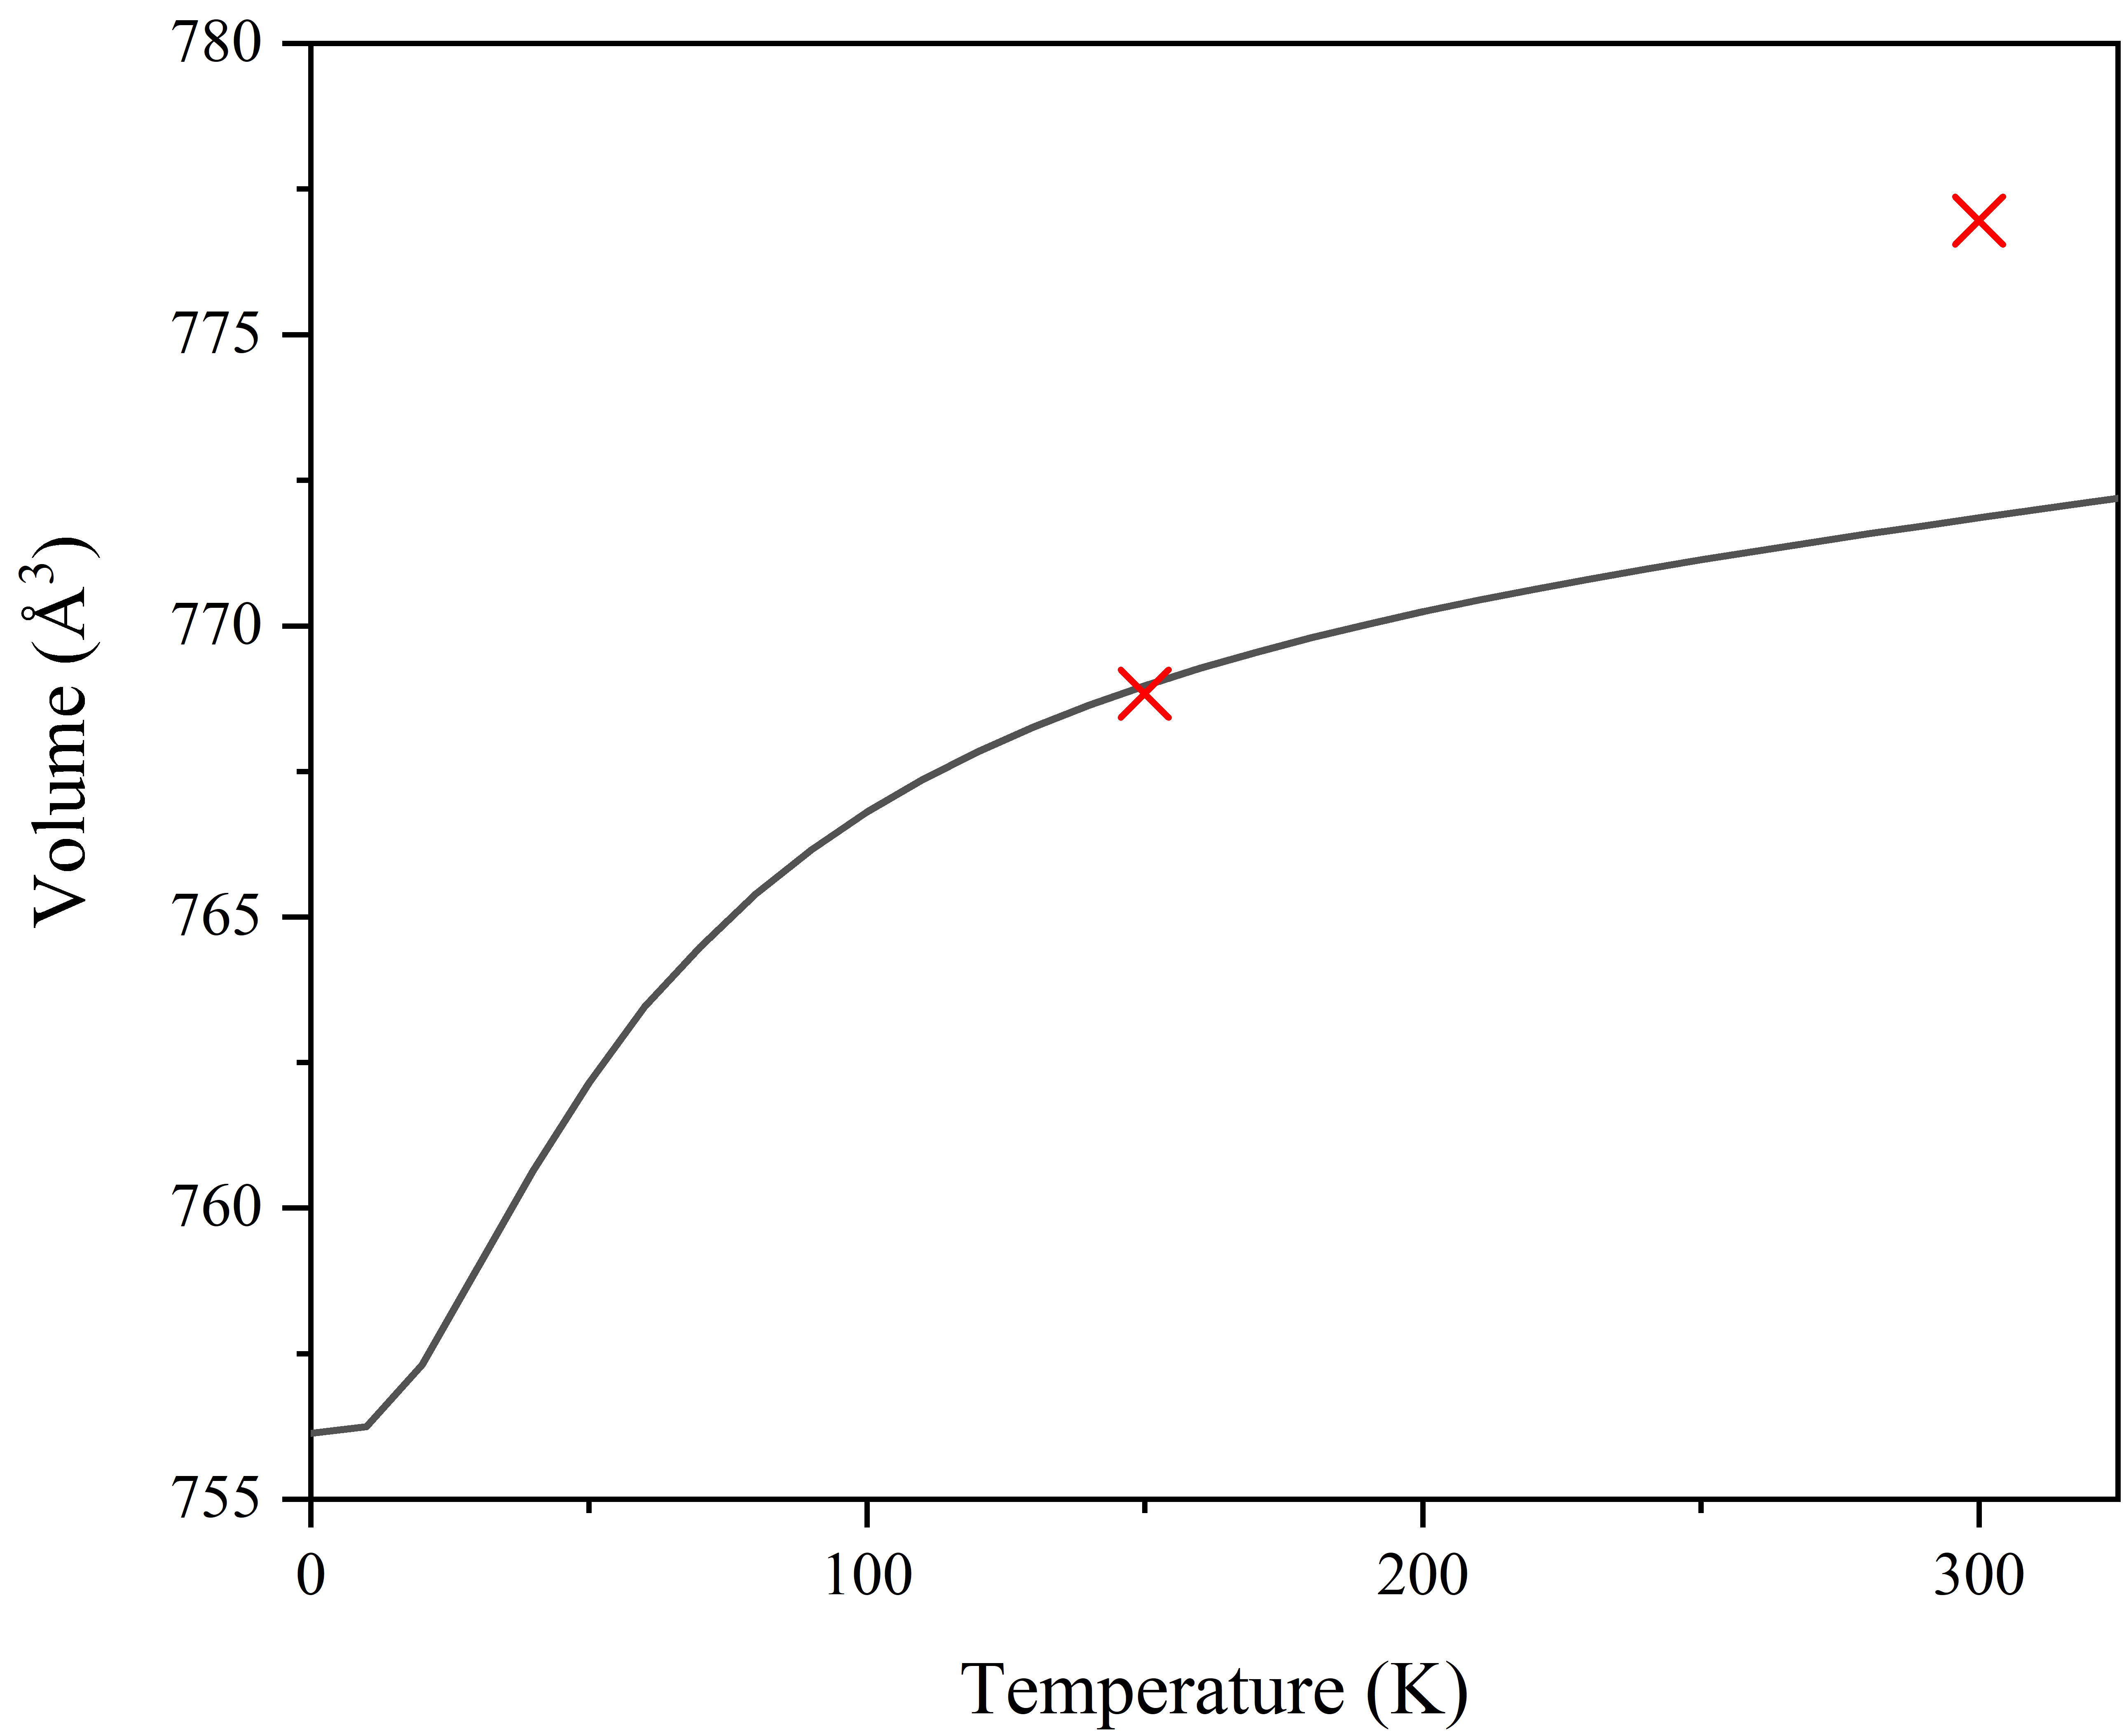
\includegraphics[width=\textwidth]{Figures/Misc/QHA/TempVolG2.png}
\caption{Temp Vol}
\label{fig:tempvol}
\end{subfigure}
\begin{subfigure}{0.49\textwidth}
\centering
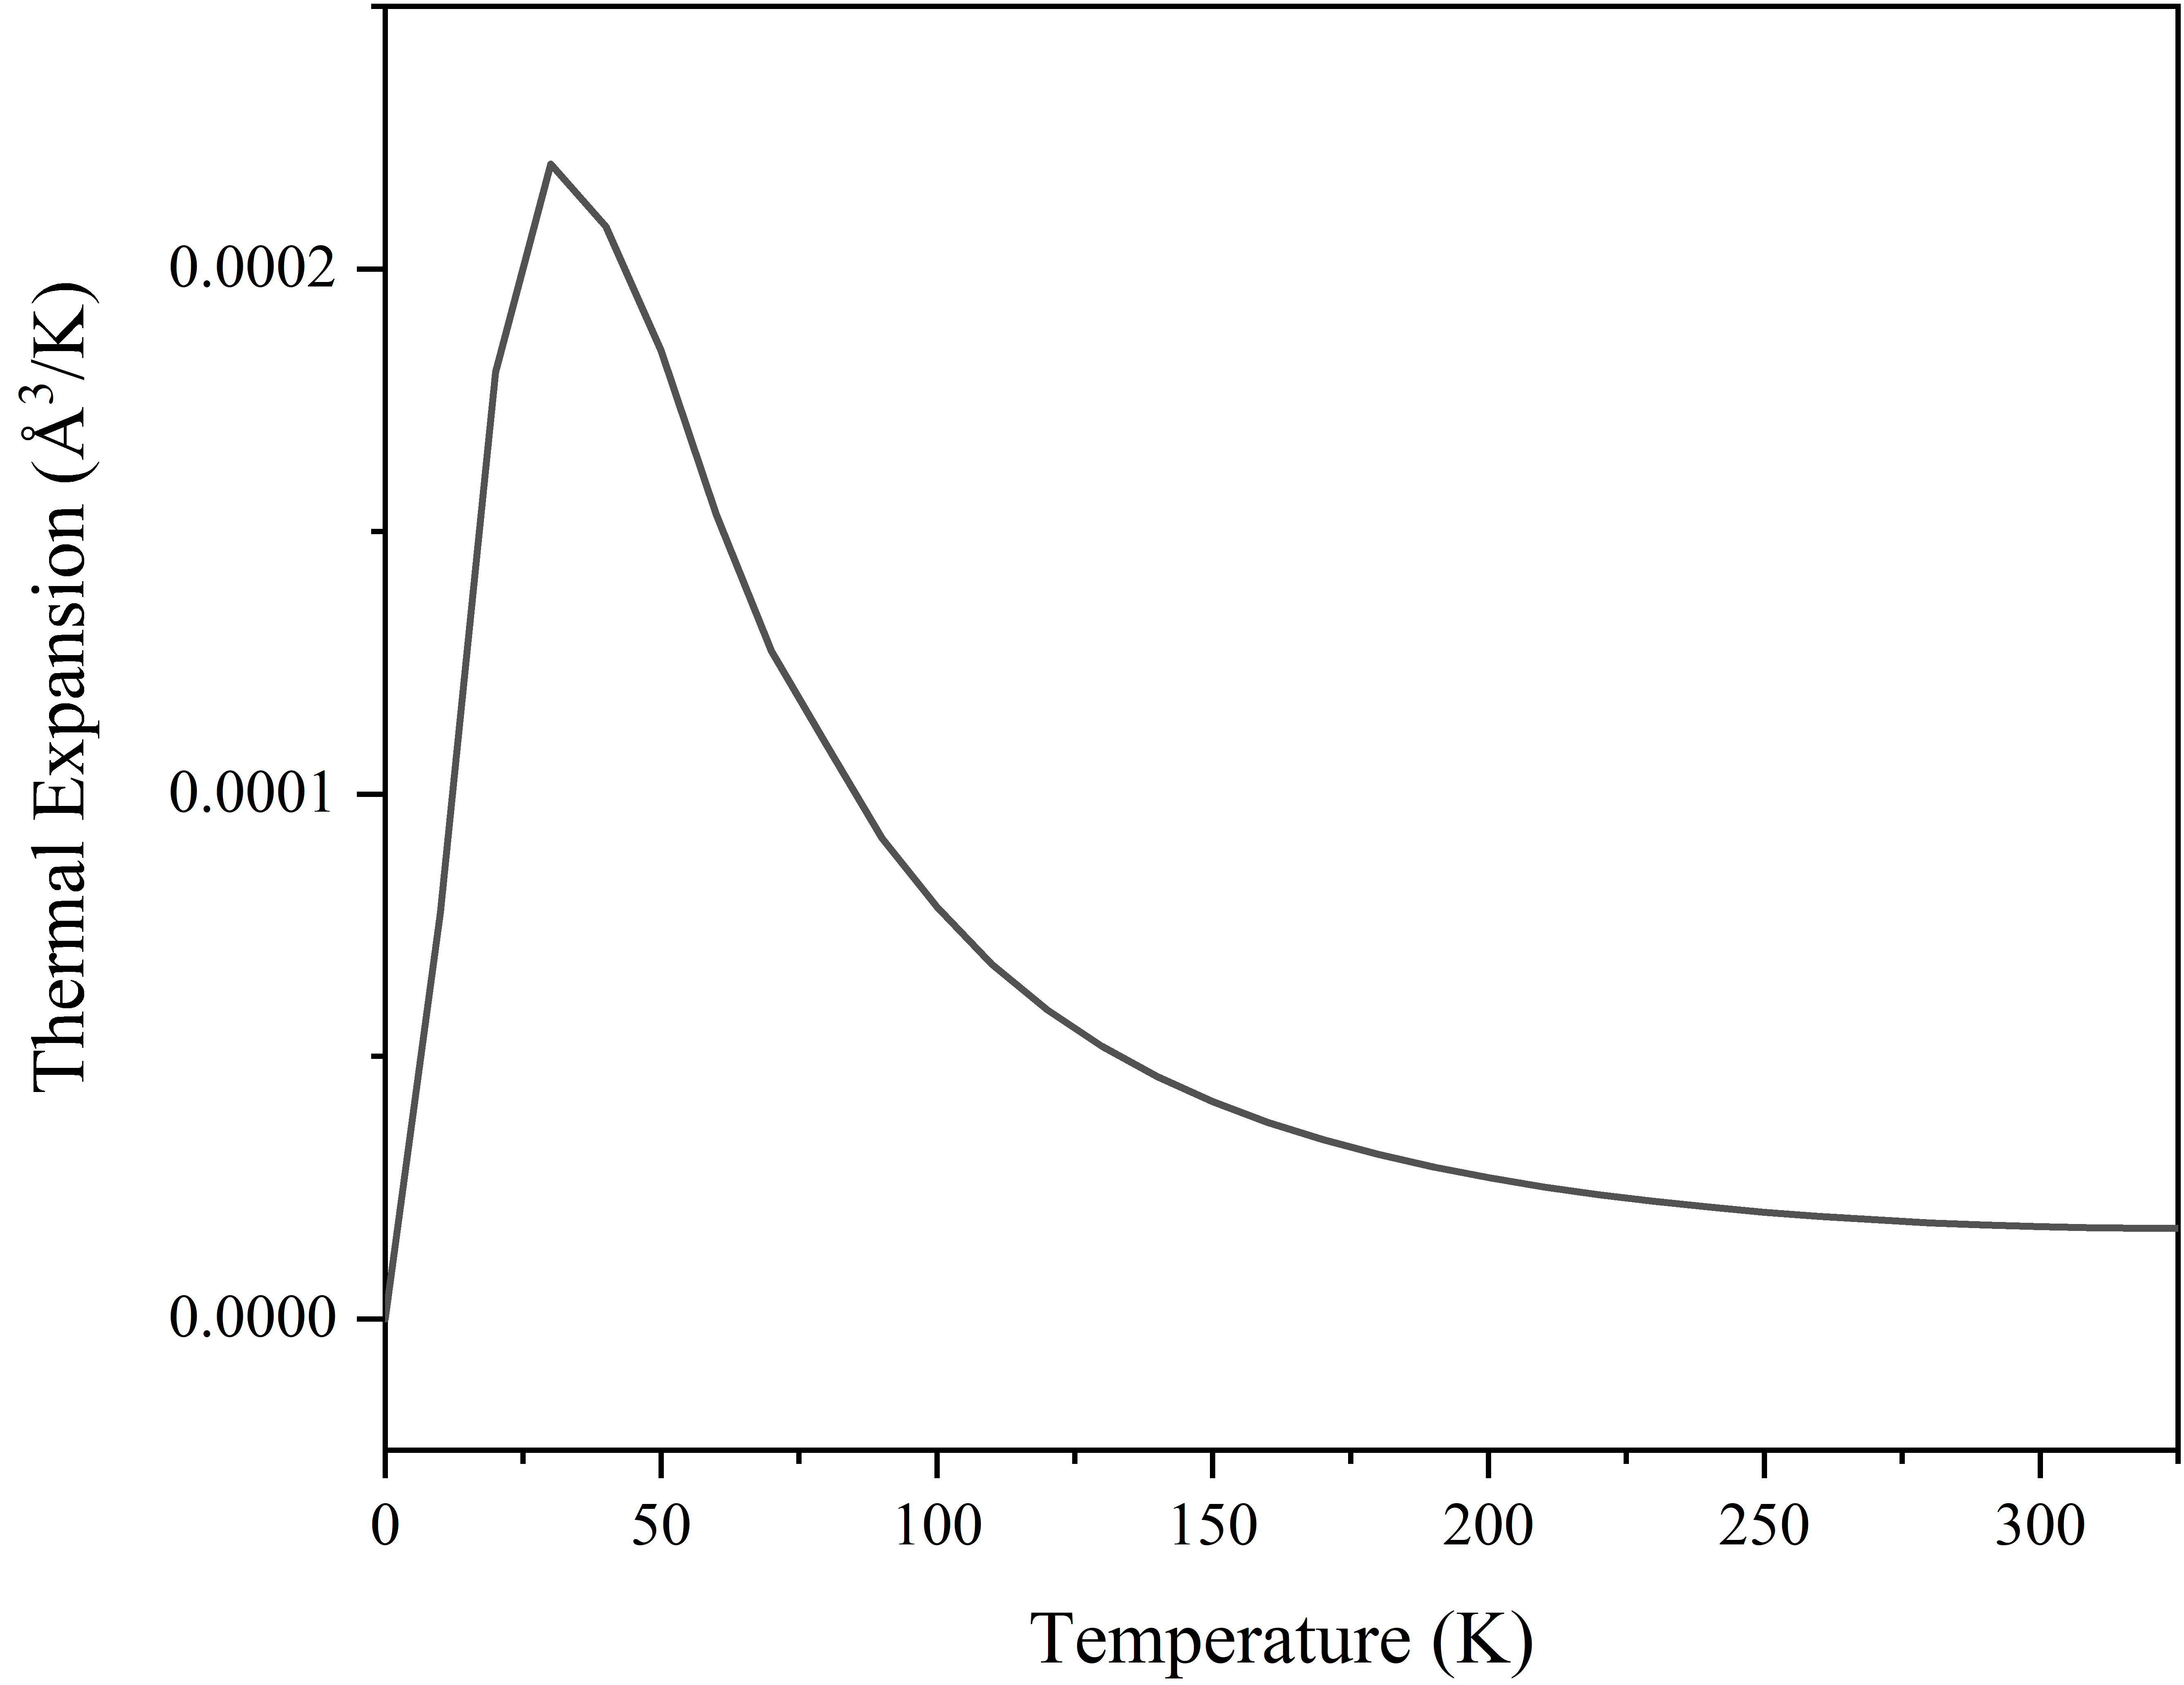
\includegraphics[width=\textwidth]{Figures/Misc/QHA/ThermExpG2.png}
\caption{Therm Exp}
\label{fig:thermexp}
\end{subfigure}

\captionsetup{font = footnotesize, justification = centering}
\caption[The Calculated Volume-Temperature Relationship and Thermal Expansion of \(\alpha\)-Lactose Monohydrate]{The calculated volume-temperature relationship and thermal expansion of \(\alpha\)-Lactose Monohydrate. This curve shows reasonable agreement with experimental values, shown in red.}
\label{Fig:tempvol+thermext}
\end{figure}

The experimental unit cell volume at \SI{150}{K} is \SI{768.84}{\angstrom^3} \cite{Smith2005} which is a difference of 0.016\% with the calculated value and the experimental volume at \SI{300}{K} is \SI{776.96}{\angstrom^3} \cite{Schreyer2014}, which is a difference of 0.66\%. Both of these differences are very small so this volume temperature curve can be assumed to be reasonably reliable up to \SI{300}{K} but this difference indicates that the thermal expansion is being underestimated to some degree. This would be confirmed by more experimental measurements of the unit cell volume at different temperatures but these were not available. Synthesis of single crystals of \acrshort{alm} and subsequent measurements by \acrshort{xrd} of the unit cell volume at a wider range of temperatures was attempted but was stopped owing to limited access to suitable facilities during the COVID pandemic.

\subsection{Heat Capacity}
Additionally, the heat capacity at constant pressure is shown in \Cref{fig:Cp}. The heat capacity shows a mostly linear trend of increasing with temperature which is expected as nearly all systems become more difficult to heat as their temperature increases. However, the experimental value at \SI{300}{K}, obtained by differential scanning calorimetry, is \SI{1.22}{J K^{-1} g^{-1}} \cite{Kawaizumi1981}, which shows significant disagreement with the calculated value of \SI{2.18}{J K^{-1} g^{-1}}. This is an increase of 78.9\%. 

Whilst the \acrshort{qha} has been used to successfully calculate the heat capacities of a range of molecular crystals \cite{Cervinka2016}, these were all small molecules when compared to \(\alpha\)\nobreakdash-Lactose and the unit cell did not contain any other species such as water. These factors will complicate the calculation process and will result in larger discrepancies between calculation and experiment. Mathews \textit{et. al.} \cite{Mathews2020} showed that the heat capacities calculated using the \acrshort{qha} begin to deviate from experiment at approximately \SI{50}{K} for various organic hydrate ices which are more comparable to \acrshort{alm} which may explain the poor experimental comparability for this calculation as \acrshort{alm} is a hydrate and incorporating the effects of the crystalline water molecules is challenging. 

\begin{figure}
\centering
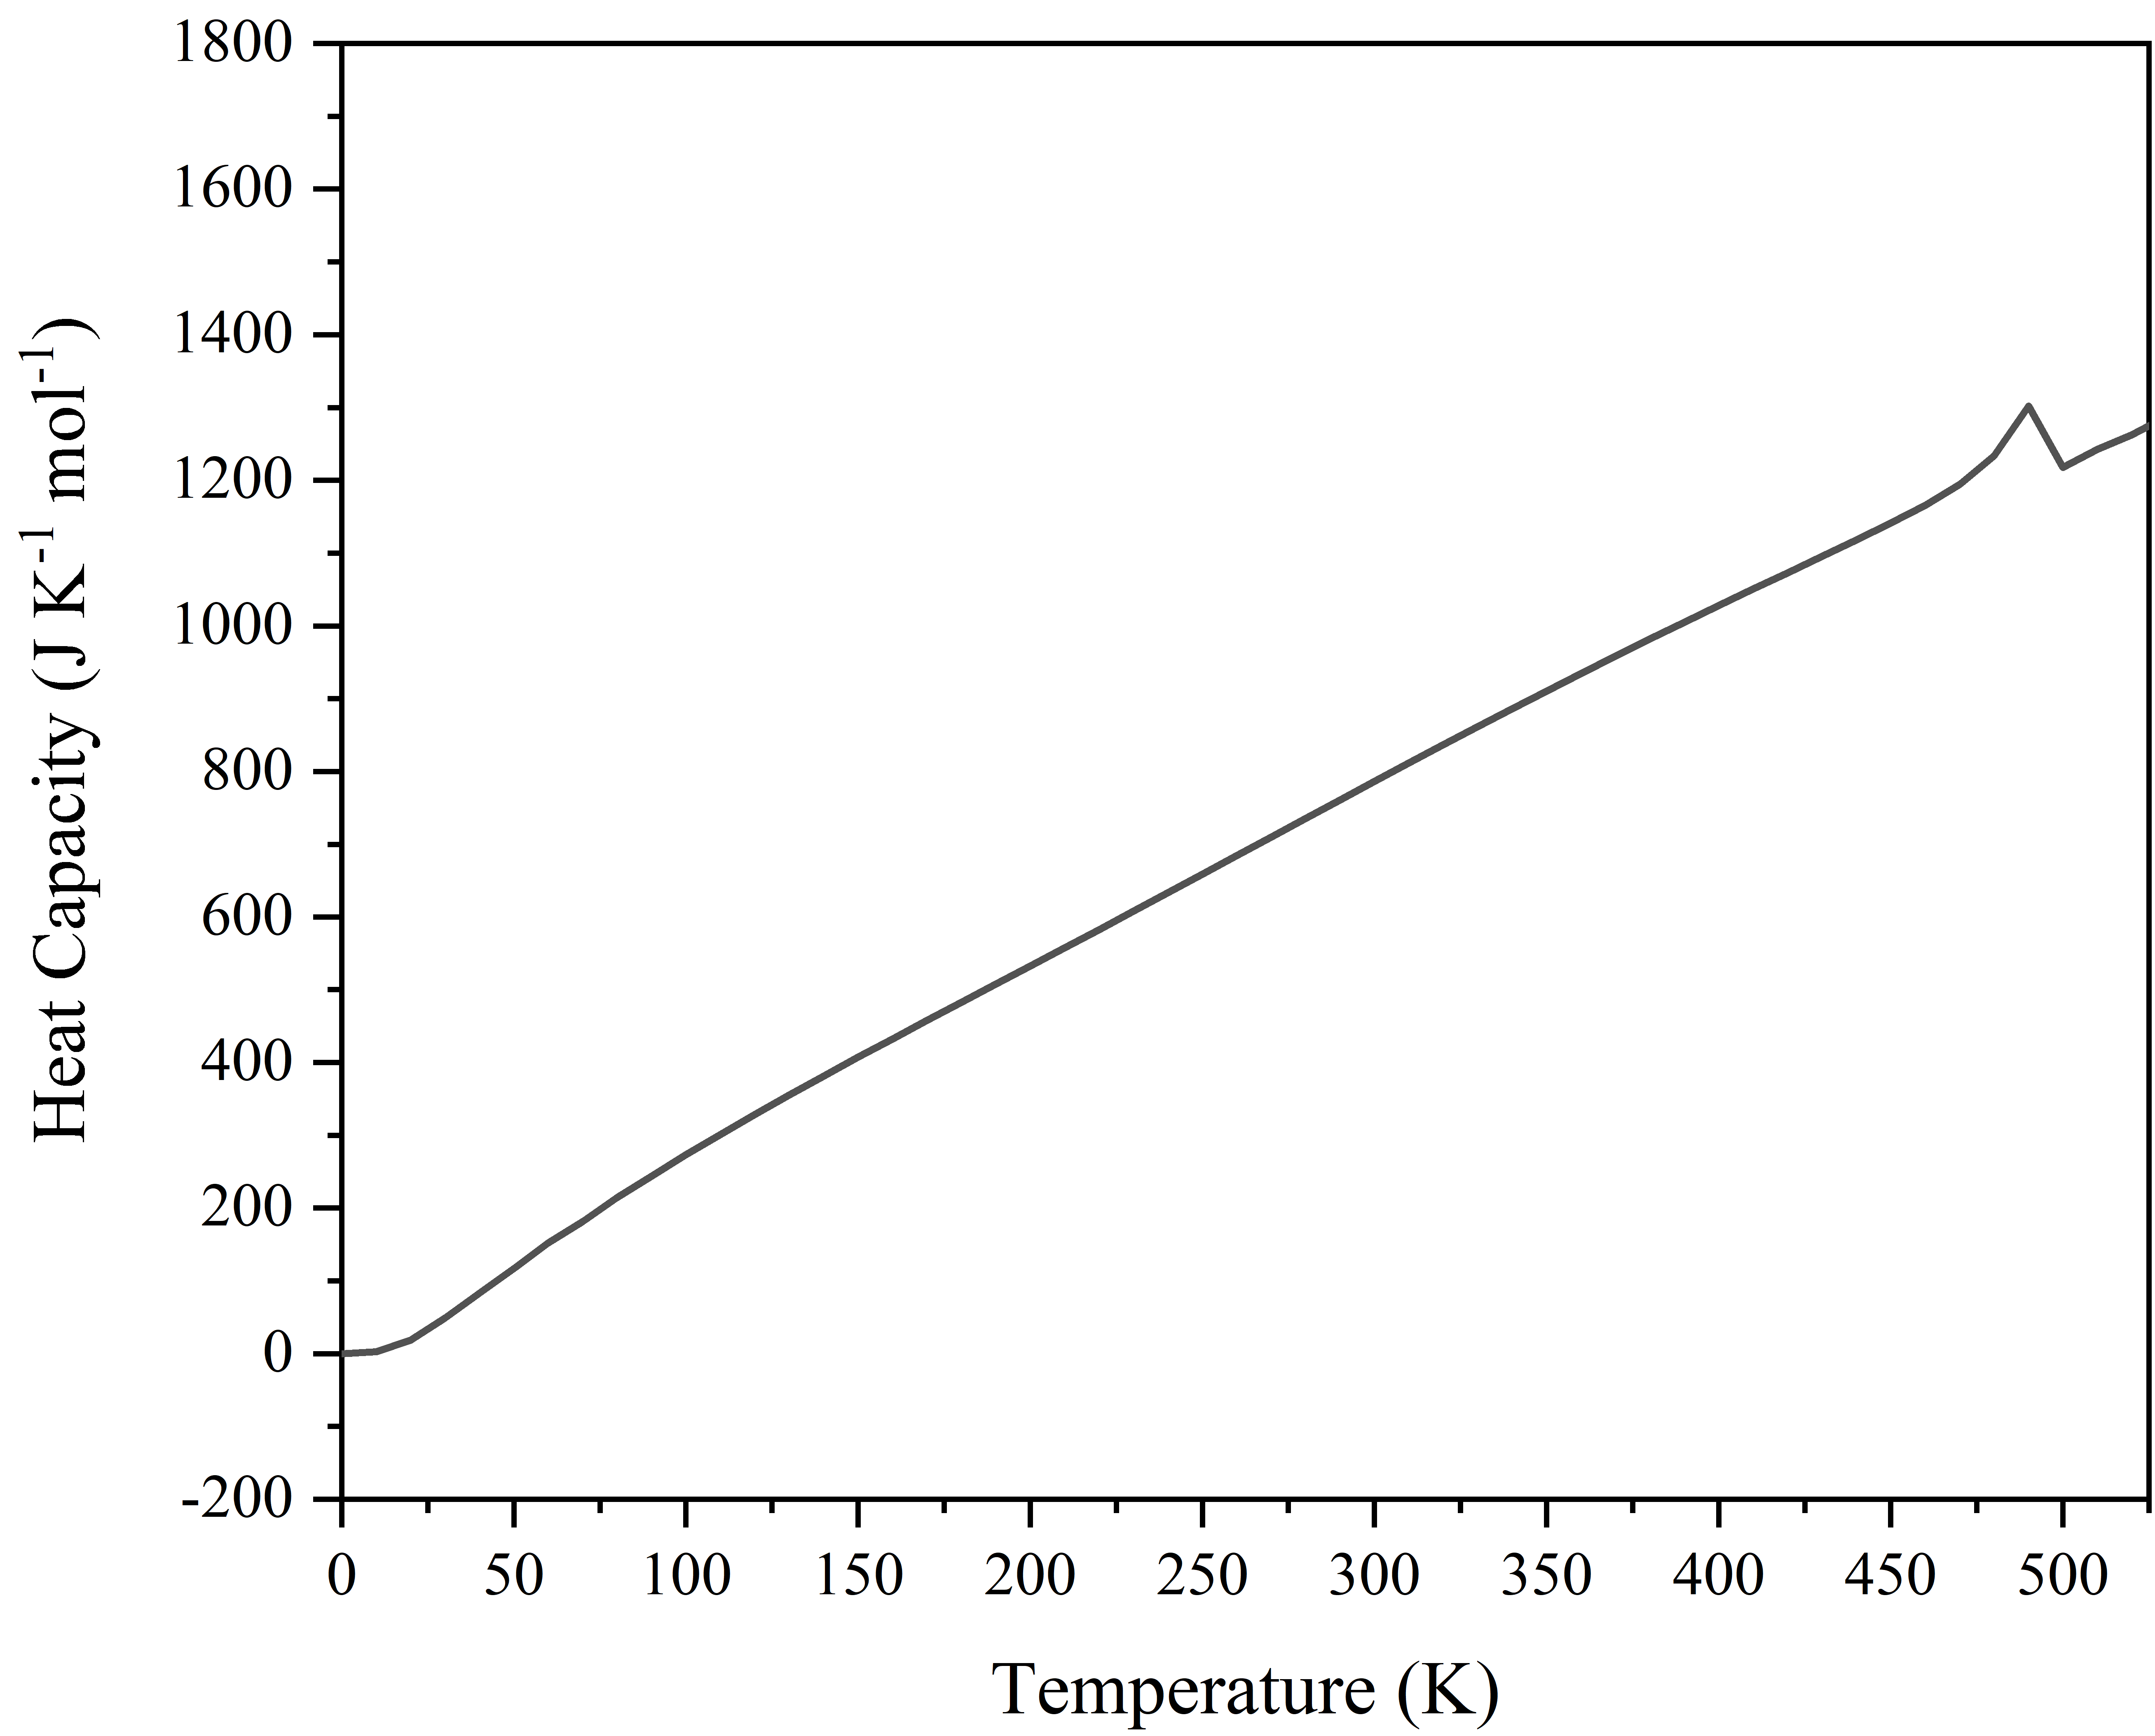
\includegraphics[width=0.5\textwidth]{Figures/Misc/QHA/CpG.png}
\captionsetup{font = footnotesize, justification = centering}
\caption[The Calculated Heat Capacity at Constant Pressure of \(\alpha\)-Lactose Monohydrate]{The calculated heat capacity at constant pressure of \(\alpha\)-Lactose Monohydrate.}
\label{fig:Cp}
\end{figure}

\section{Temperature Dependence of Calculated Terahertz Spectra}
\subsection{Temperature Dependence of Phonon Frequency}
Now that the volume of the unit cell has been calculated as a function of temperature, it is possible to calculate the dynamical matrix, and therefore phonon properties, at different temperatures. This was done by creating structures with a unit cell volume corresponding to a particular temperature from \Cref{fig:tempvol} and optimising the ionic positions. The calculated frequencies for the modes selected in \Cref{Fig:d3_exp_mode_temp} as a function of temperature are shown in \Cref{Fig:ModeTempShift}, alongside the experimental frequencies and the frequency calculated without using the \acrshort{qha}.

\begin{figure}
\centering

\begin{subfigure}{0.45\textwidth}
\centering
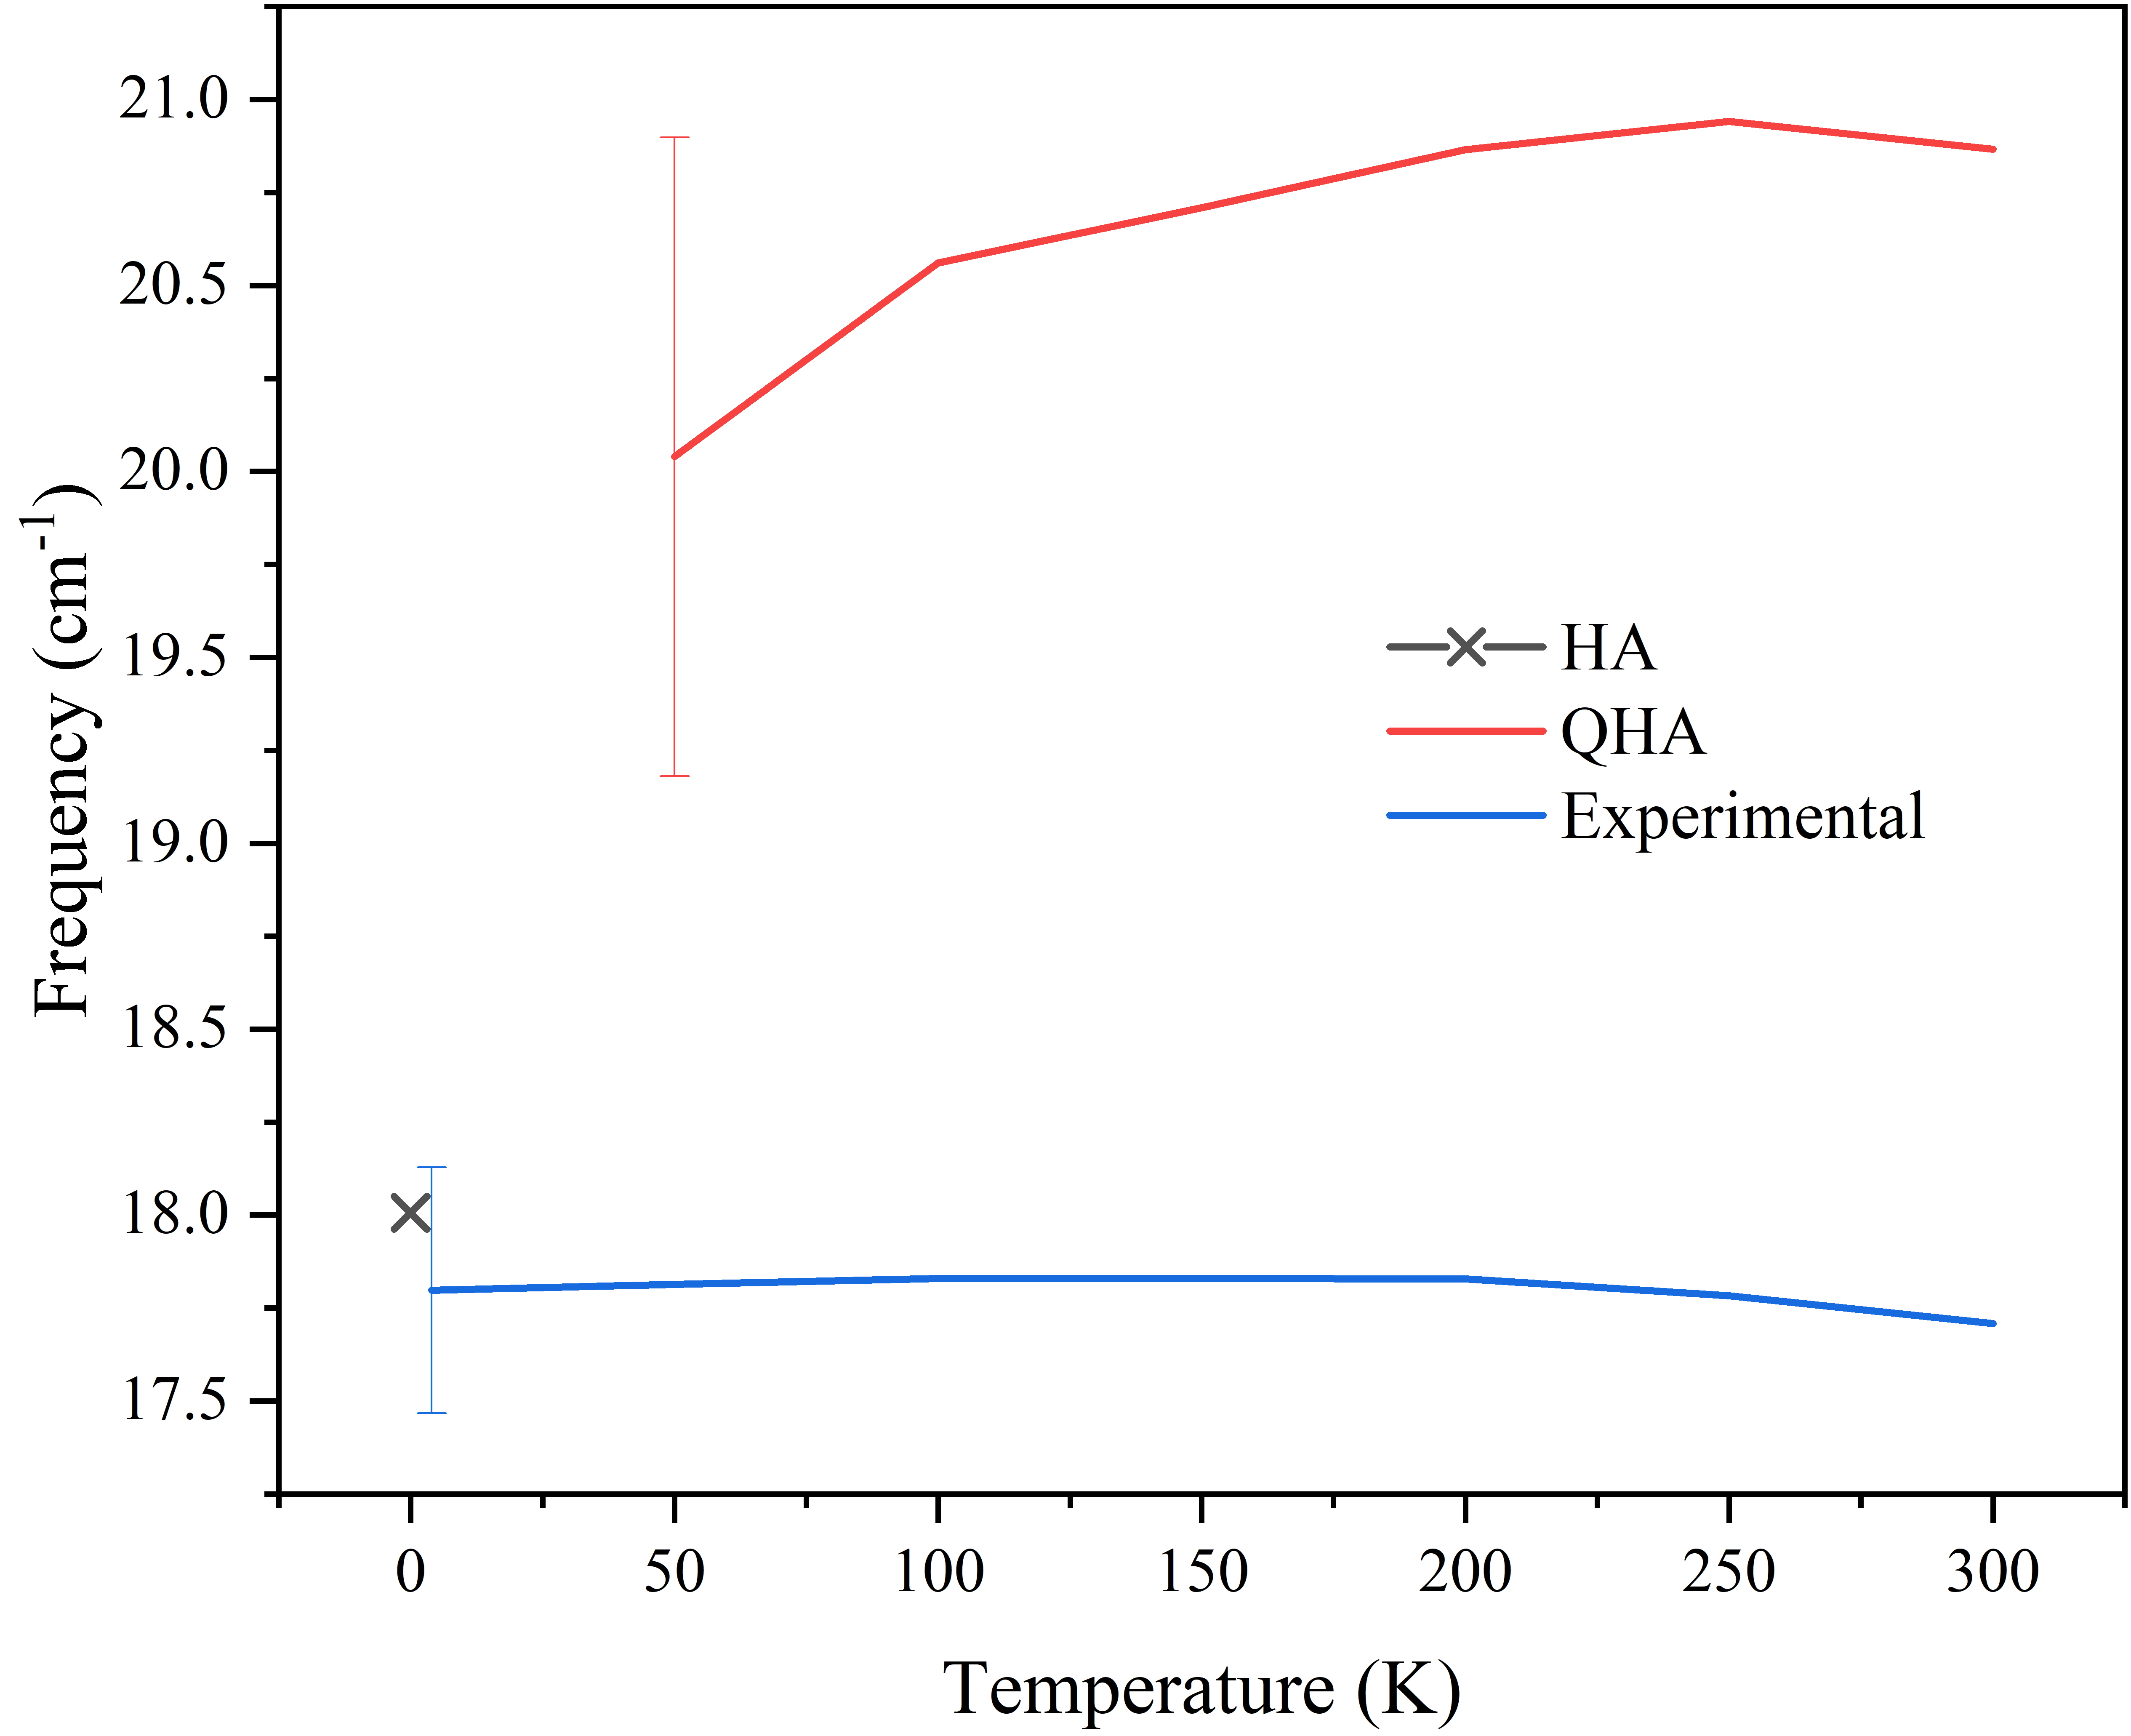
\includegraphics[width=\textwidth]{Figures/Misc/QHA/Mode1CompV2G2.png}
\caption{Mode 1 Temperature Dependence}
\label{fig:mode1temp}
\end{subfigure}
\begin{subfigure}{0.45\textwidth}
\centering
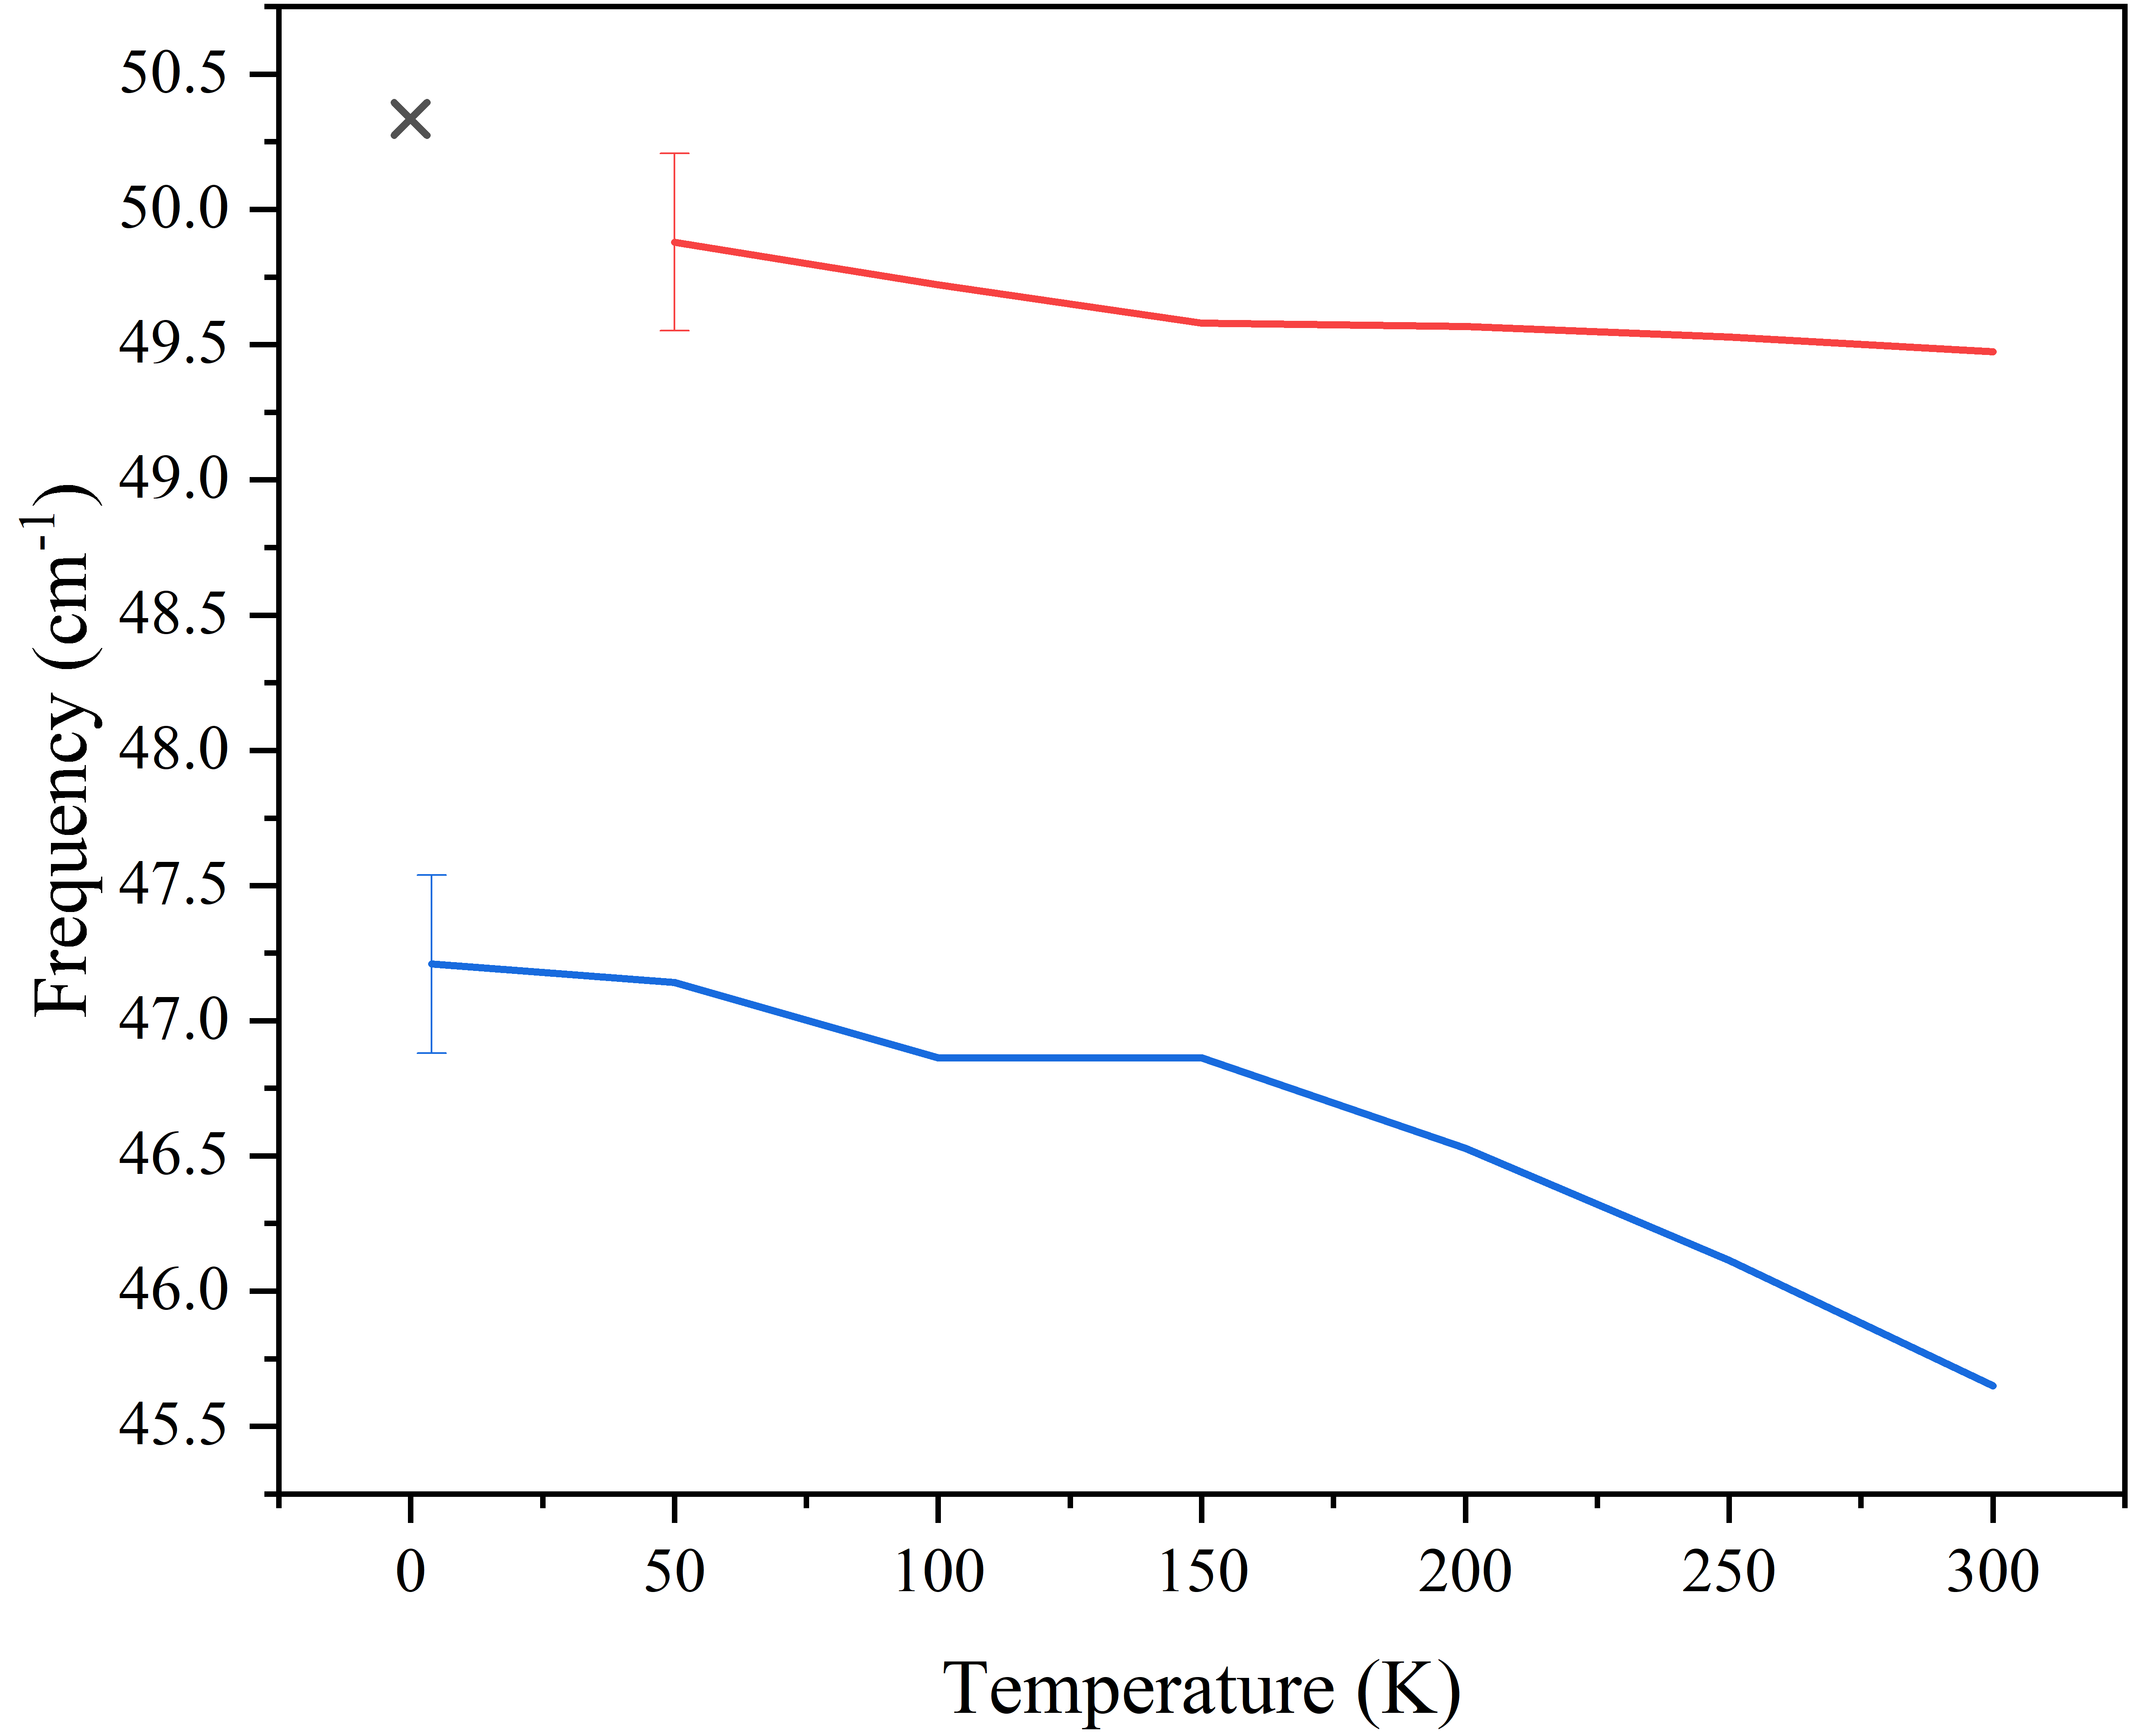
\includegraphics[width=\textwidth]{Figures/Misc/QHA/Mode2CompV2G.png}
\caption{Mode 2 Temperature Dependence}
\label{fig:mode2temp}
\end{subfigure}

\begin{subfigure}{0.45\textwidth}
\centering
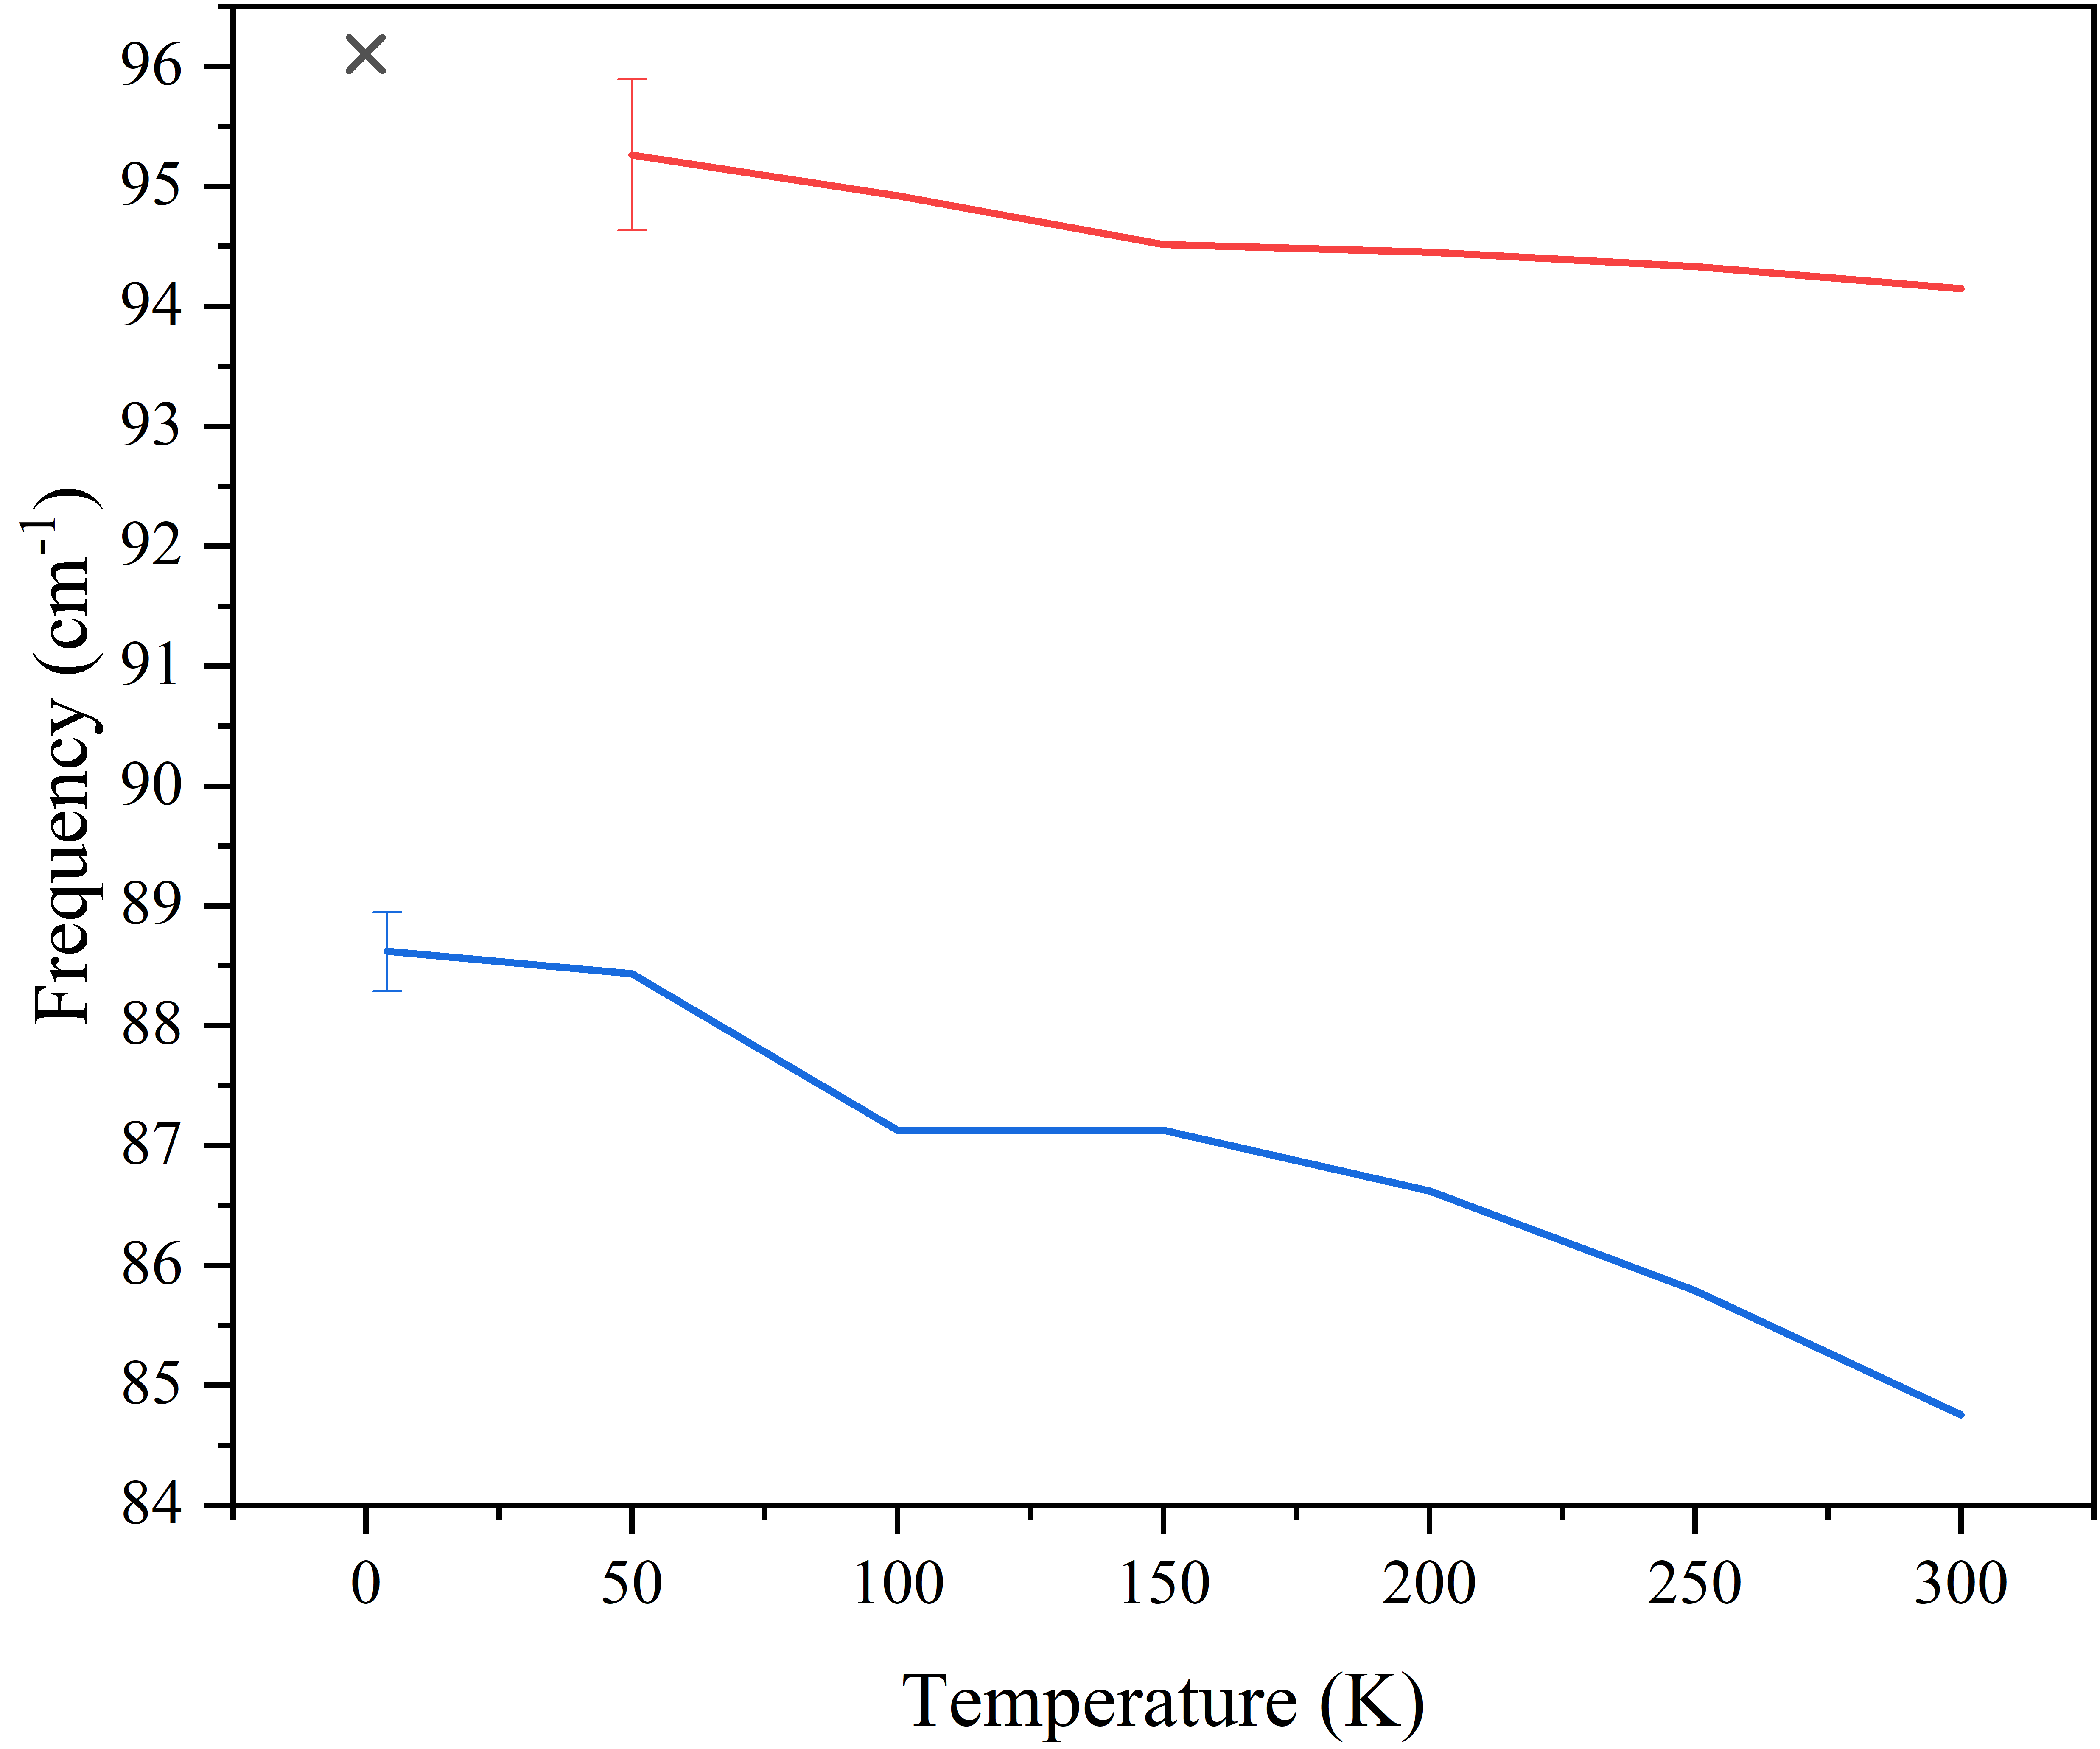
\includegraphics[width=\textwidth]{Figures/Misc/QHA/Mode3CompV2G.png}
\caption{Mode 3 Temperature Dependence}
\label{fig:mode3temp}
\end{subfigure}
\begin{subfigure}{0.45\textwidth}
\centering
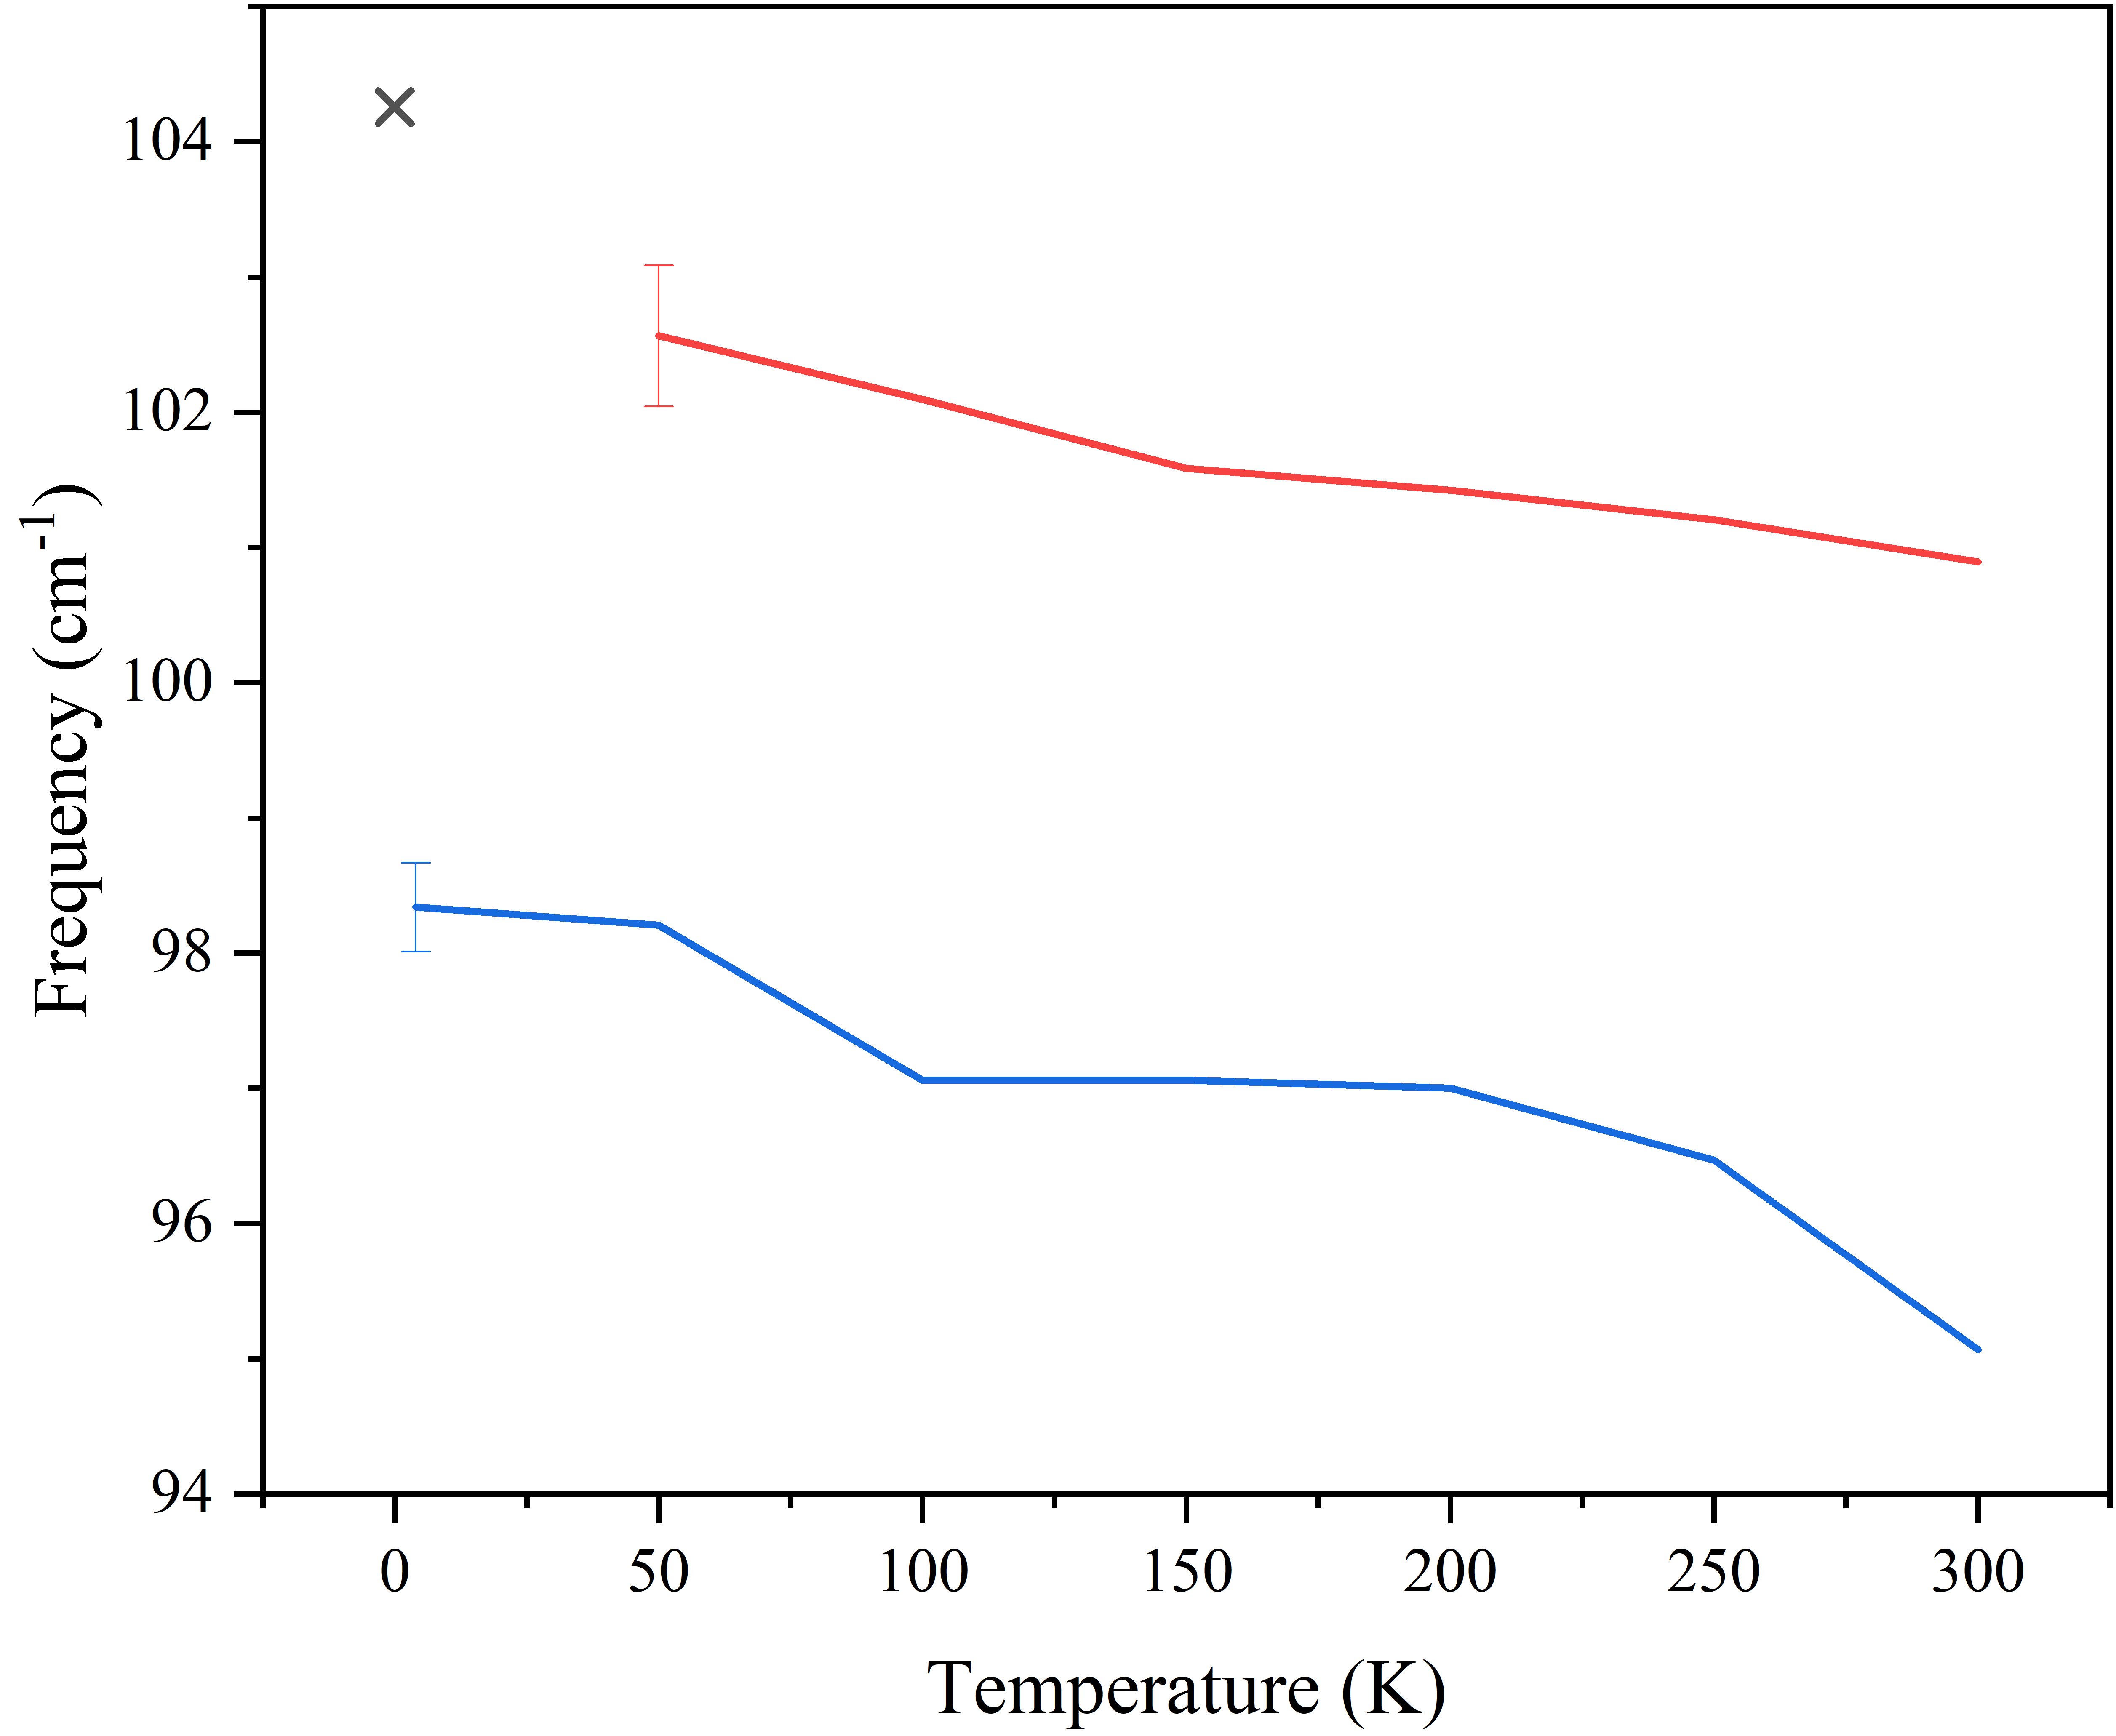
\includegraphics[width=\textwidth]{Figures/Misc/QHA/Mode4CompV2G.png}
\caption{Mode 4 Temperature Dependence}
\label{fig:mode4temp}
\end{subfigure}

\begin{subfigure}{0.45\textwidth}
\centering
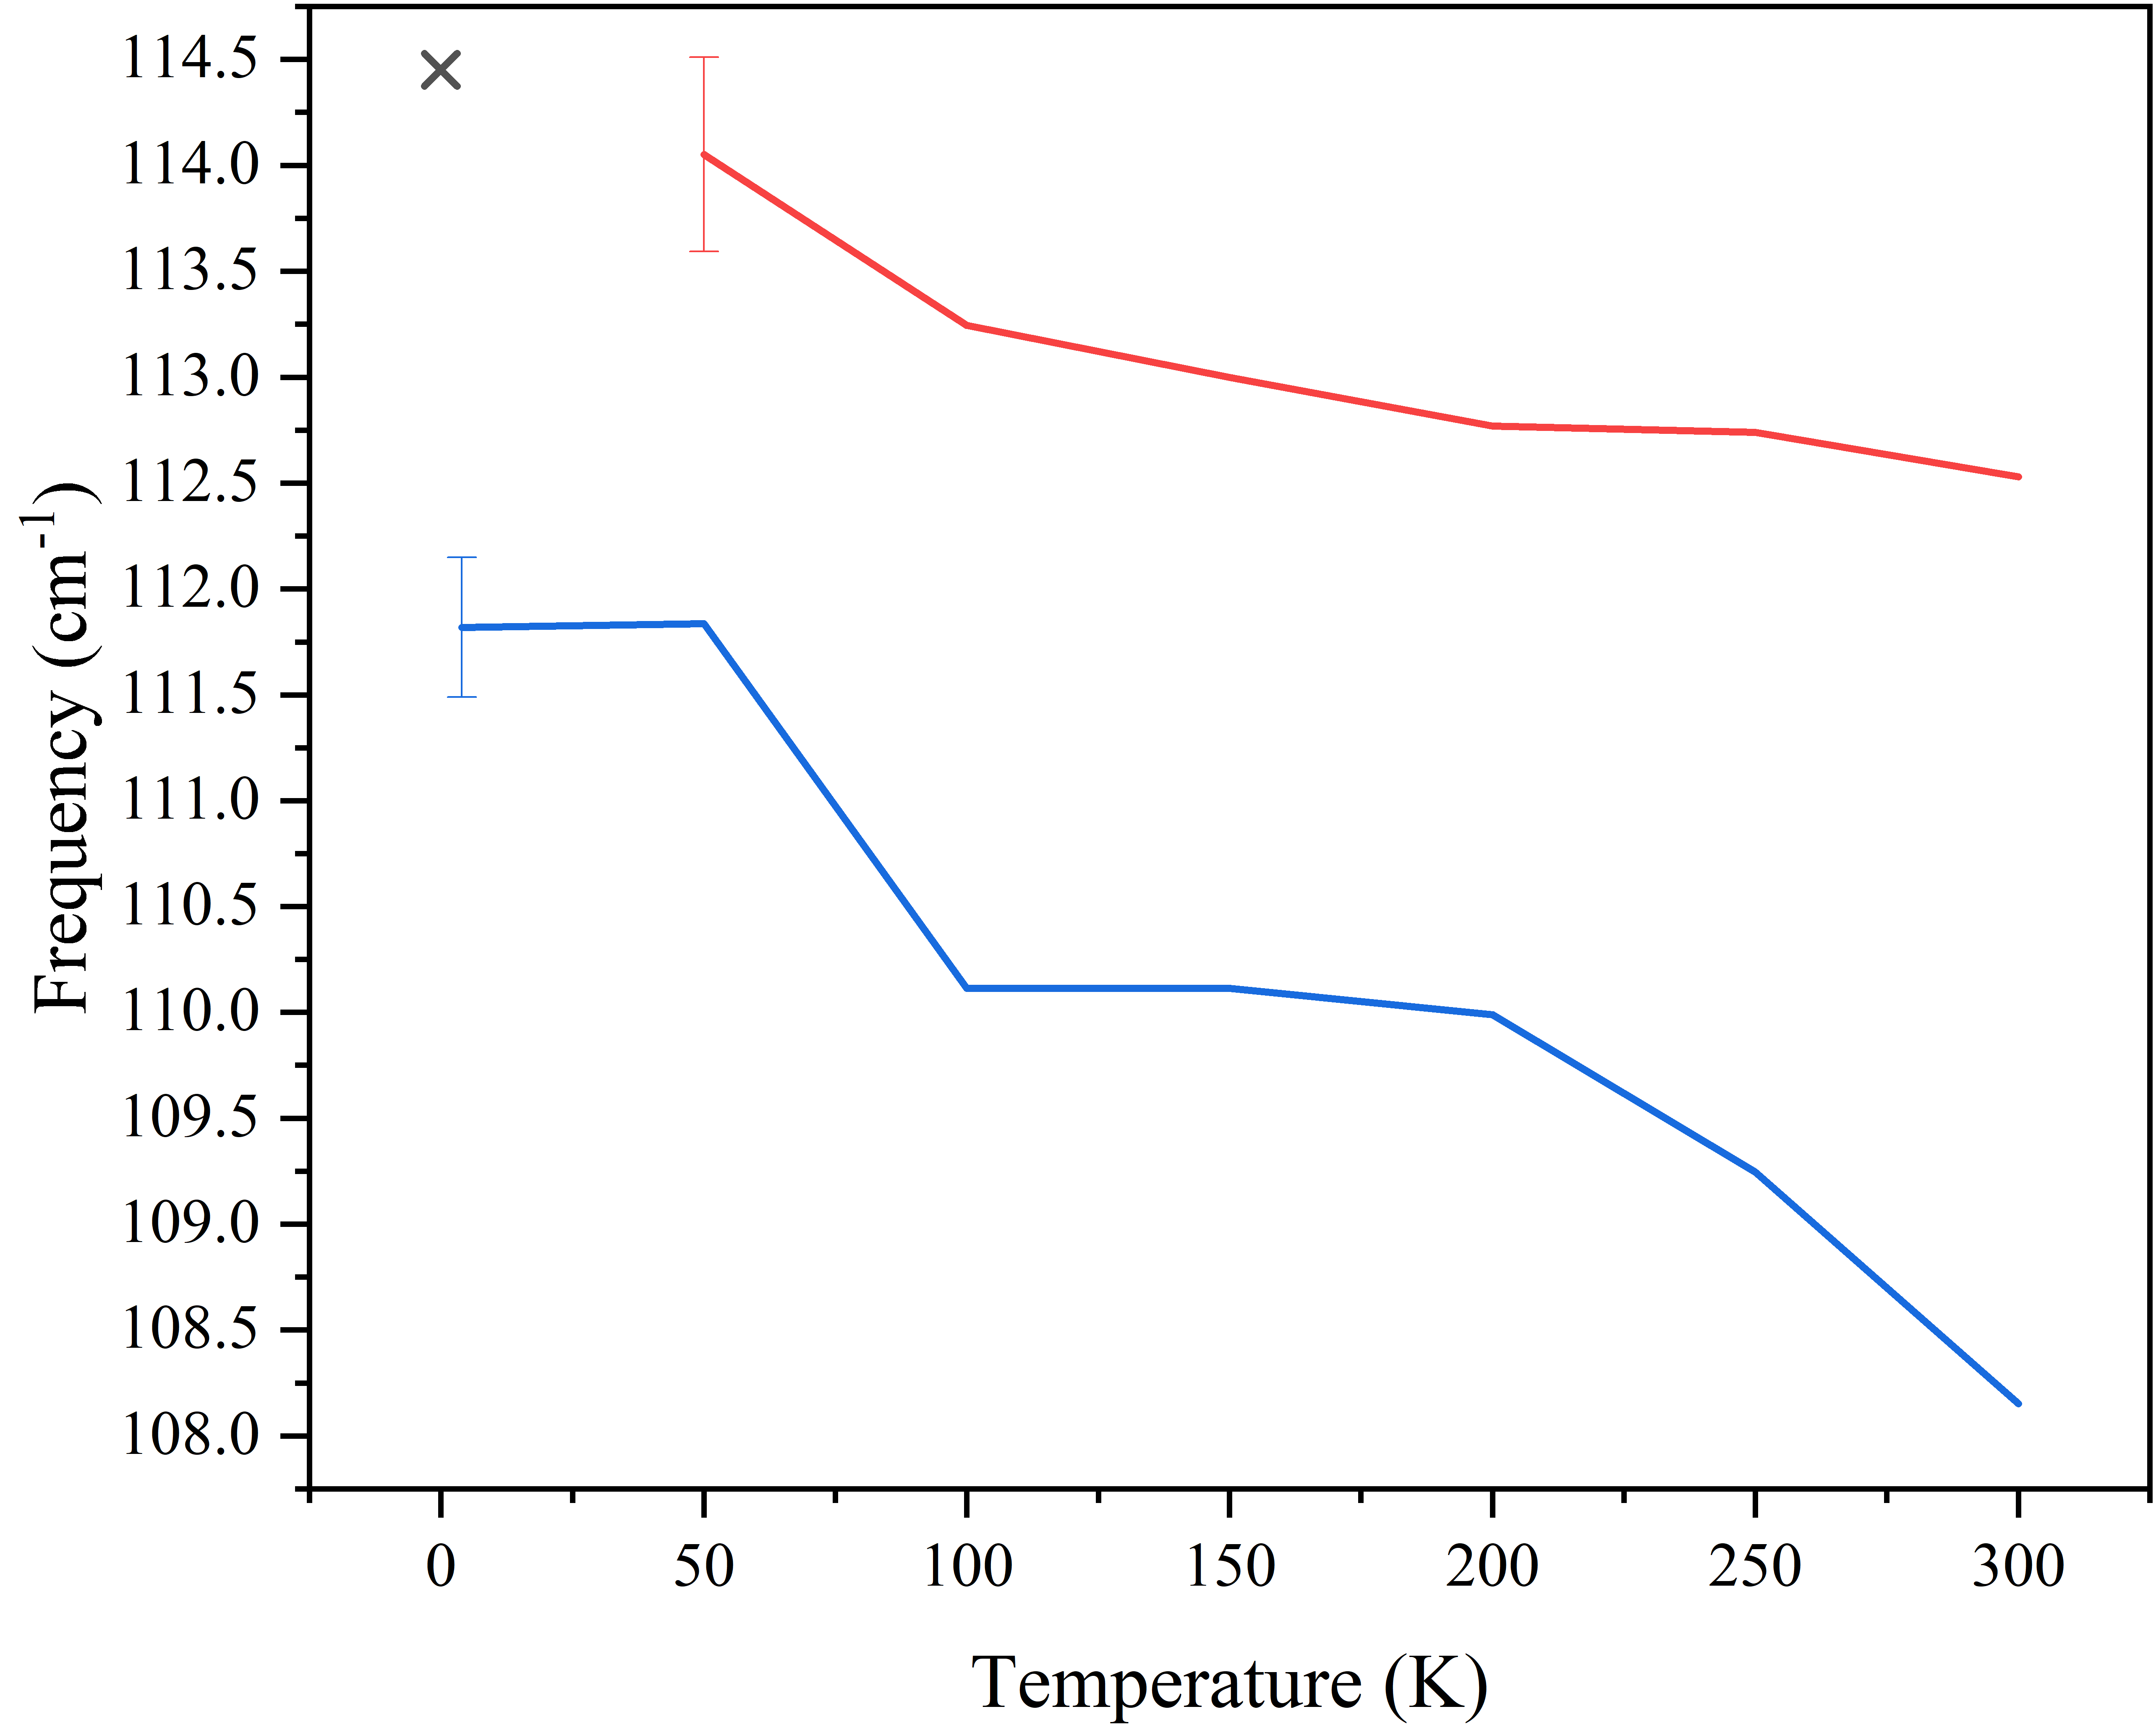
\includegraphics[width=\textwidth]{Figures/Misc/QHA/Mode5CompV2G.png}
\caption{Mode 5 Temperature Dependence}
\label{fig:mode5temp}
\end{subfigure}
\captionsetup{font = footnotesize, justification = centering}
\caption[The Calculated and Experimental Mode Frequencies as a Function of Temperature]{The calculated and experimental mode frequencies as a function of temperature. All modes show an expected trend of decreasing frequency with temperature with the exception of Mode~1. The error bars arise from the standard deviation of multiple identical calculations, assumed to be similar across the temperature range, and the experimental frequency resolution. }
\label{Fig:ModeTempShift}
\end{figure}

This was partially successful with the correct trend of frequency decreasing with temperature was predicted for Mode~2 to Mode~5. However, there are disagreements of up to nearly \SI{10}{cm^{-1}} which is over 10\% of the value and would be considered a large discrepancy. This discrepancy seems to increase with temperature for all modes. The large disagreement for Mode~3 is similar to that shown in \Cref{subsec:ivdw_modeanal} where it was also poorly represented by the \acrshort{ho}. For Mode~1 however, these calculations were less successful. Whilst Mode~1 does not change with temperature experimentally, it has been calculated to slightly increase with temperature. The error bar shown on the red trace is the standard deviation of this mode's frequency, calculated using the calculations presented in \Cref{sec:simstud} and the error bar on the blue trace is the experimental frequency resolution which is \SI{0.33}{cm^{-1}}. It is assumed that the calculated error is similar across all temperatures. For Mode~1, it is possible that this temperature shift is just within the margin of error for these calculations but if this is not the cause then this mode has been poorly modelled owing to the rarity of a positive frequency shift with temperature and this does not agree with experiment. Additionally, Mode~2 was calculated to have a very slight temperature dependence which matches experiment but is close to being within the margin of error for these calculations. All mode frequencies were overestimated when compared to their experimental values. Mode~2 through to Mode~5 have temperature dependencies that are smaller than their experimental counterparts which manifests as a shallower gradient with the possible exception of Mode~4 which has the best overall correlation with experiment.

The mode Gr\"uneisen parameter is a quantity that describes how a given mode's frequency will change with the volume of the unit cell. When considering the harmonic approximation, the mode Gr\"uneisen parameter should be zero for every mode as the restoring force acting on an ion or molecule will be linear. By varying the volume and using the \acrshort{qha}, the mode Gr\"uneisen parameter can be calculated and these are shown for modes up to \SI{3.5}{\acrshort{thz}} in \Cref{fig:gruns} where the modes in red ``+'' symbols are Mode~1 to Mode~5 for clarity. A positive value indicates that the frequency decreases with temperature and a larger value indicates that the frequency will decrease more rapidly with temperature. Conversely, a negative value indicates that the frequency will increase with temperature. These values corroborate the trends seen in \Cref{Fig:ModeTempShift}, with Mode~4 having the greatest frequency shift with temperature and Mode~1 having a negative mode Gr\"uneisen parameter. The value is large owing to the low frequency in this mode and so any shift is proportionally larger.

\begin{figure}[h]
\centering
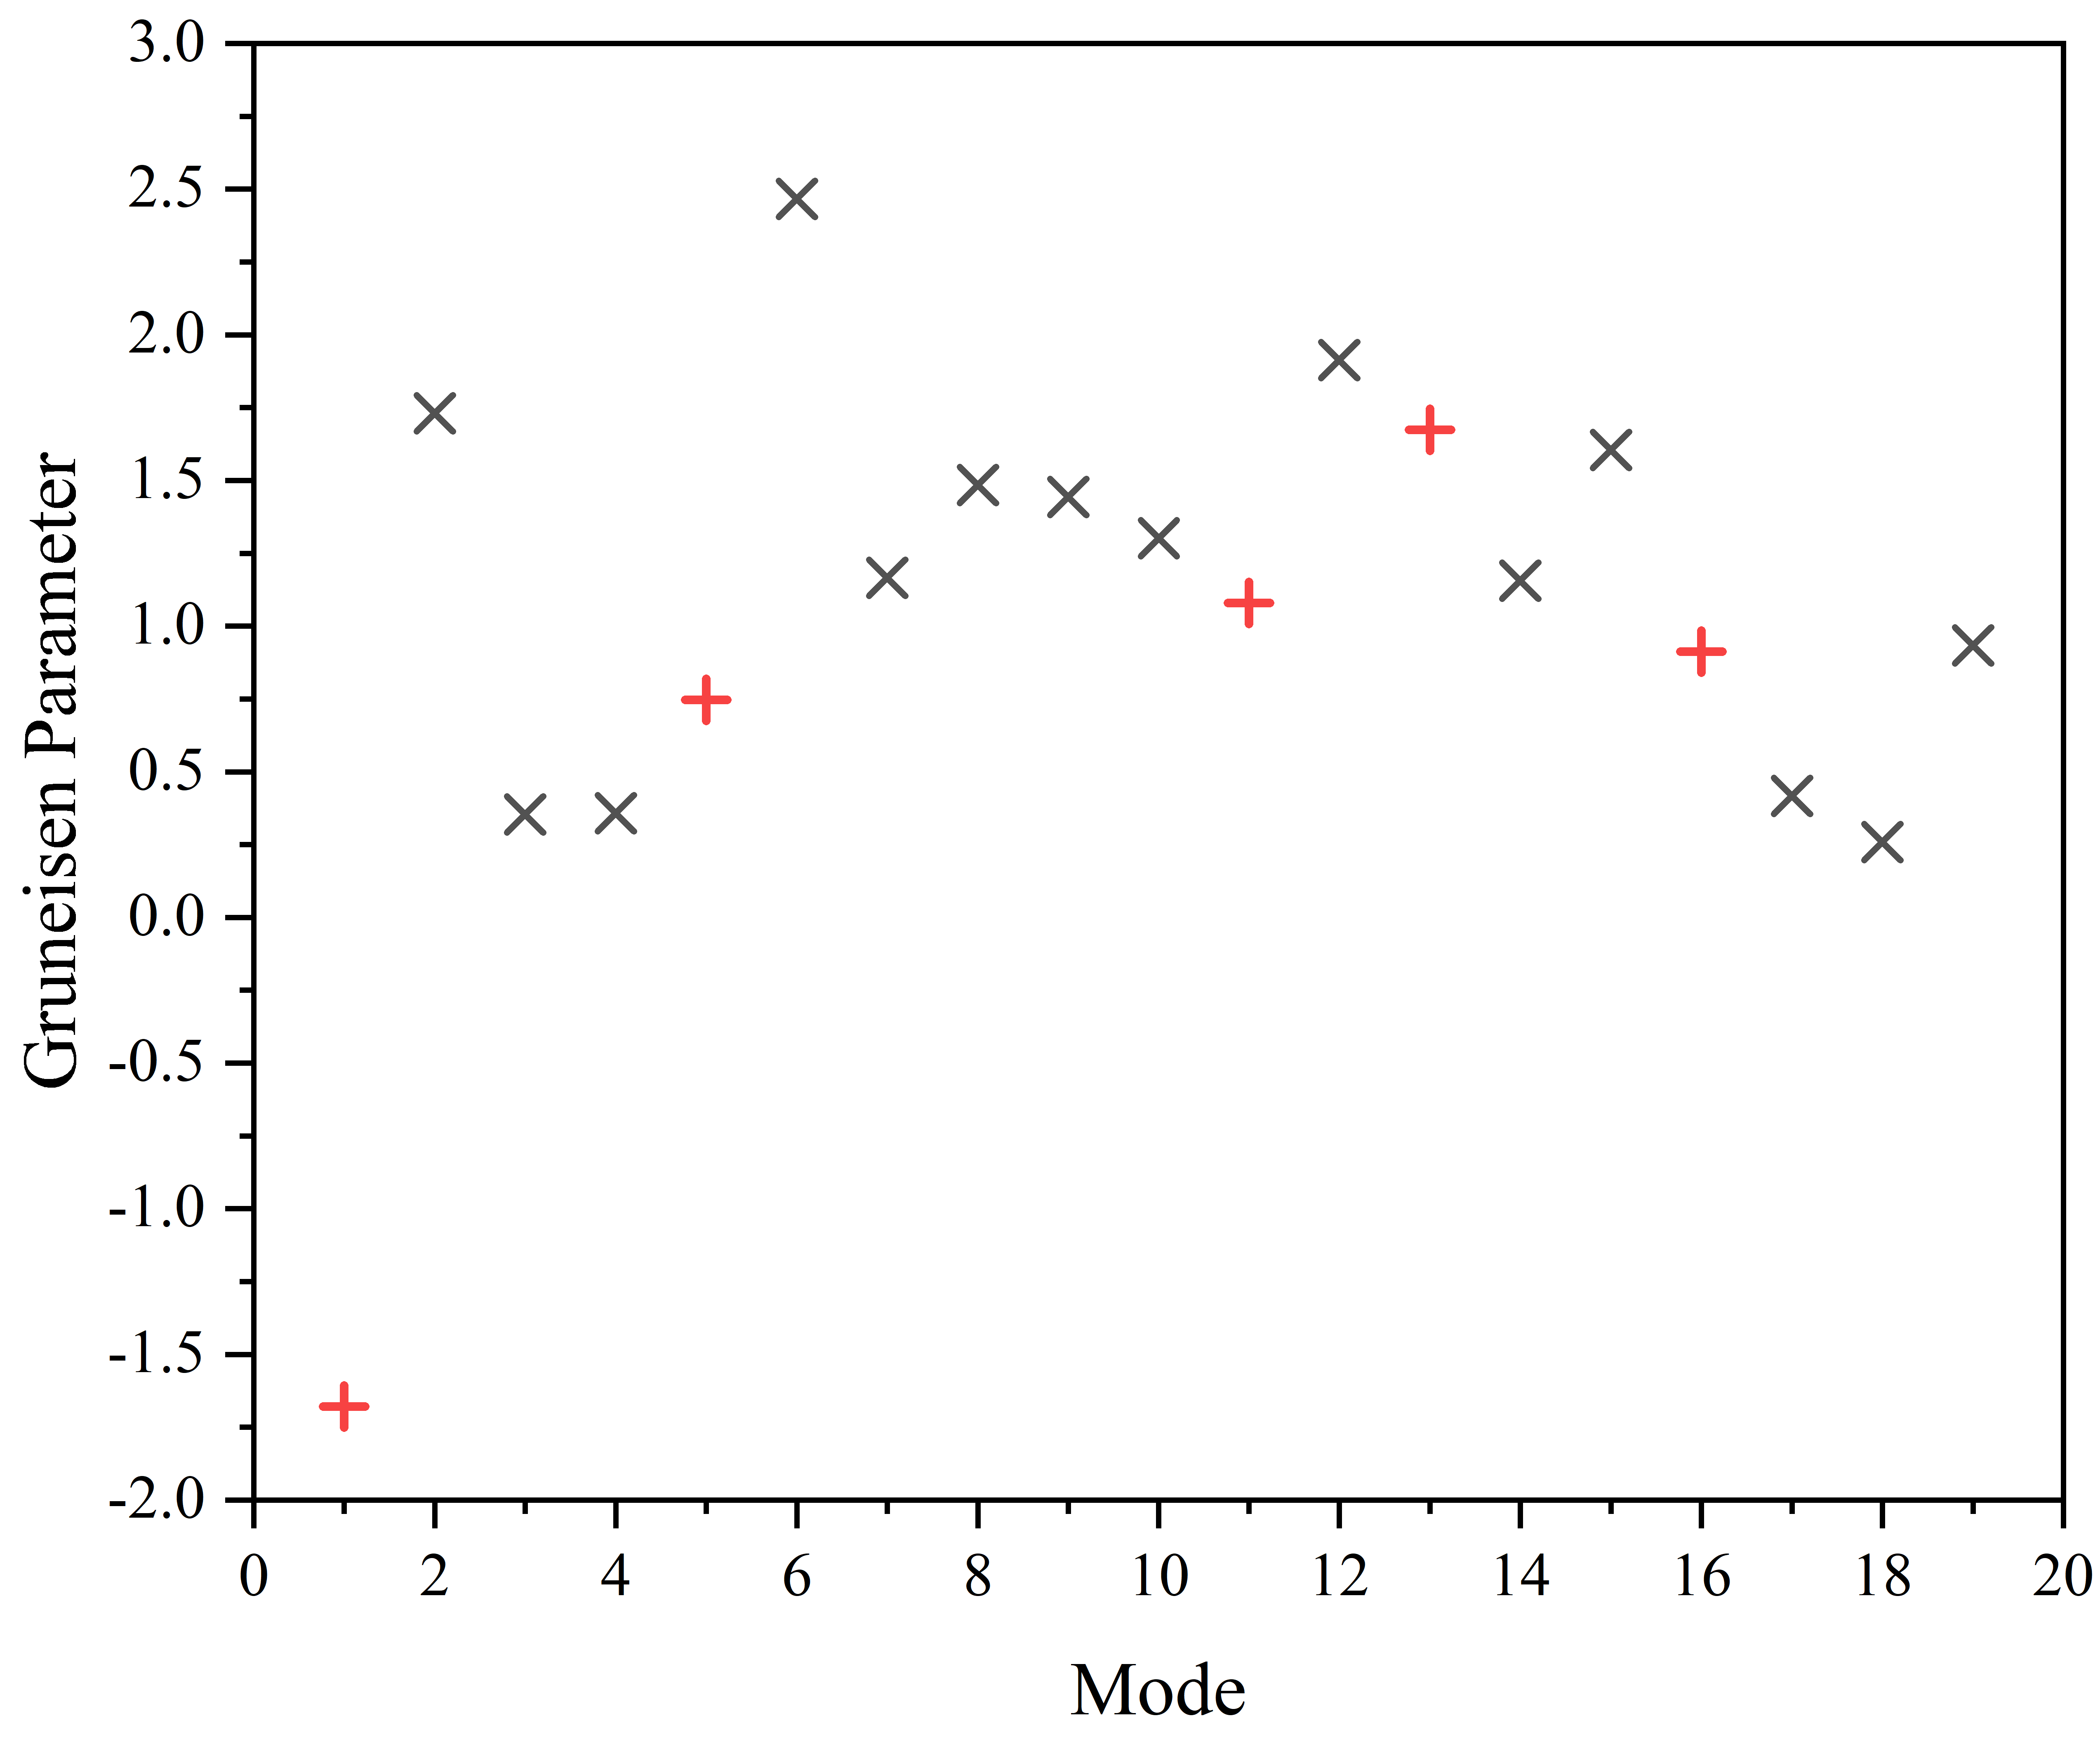
\includegraphics[scale=0.5]{Figures/Misc/QHA/GrunsModeG.png}
\captionsetup{font = footnotesize, justification = centering}
\caption[The Calculated Mode Gr\"uneisen Parameters for \(\alpha\)-Lactose Monohydrate]{The calculated mode Gr\"uneisen parameters for each mode of \(\alpha\)-Lactose Monohydrate under \SI{125}{cm^{-1}}. The only mode with a negative mode Gr\"uneisen parameter is Mode~1.}
\label{fig:gruns}
\end{figure}

\subsection{Calculation of Terahertz Absorption Spectrum at Room Temperature}
Now that the unit\nobreakdash-cell volume at \SI{300}{K} is known, a structure that has this volume can be created. The atomic positions can then be optimised, without altering the unit\nobreakdash-cell dimensions, and the dynamical matrix can be calculated to produce a calculated \acrshort{thz} absorption spectrum that should more closely represent the experimental spectrum at \SI{300}{K}. These are both shown in \Cref{Fig:RTvsEXP}, where the 300 and \SI{4}{K} spectra are shown for comparison. This was achieved using experimental peak widths for the five major peaks and a default peak width of \SI{5}{cm^{-1}}, an air void radius of \SI{10}{\micro\metre} and void volume fraction of 7\%. This was selected to best match the rising background absorption at approximately \SI{3}{\acrshort{thz}} and is larger than was used in \Cref{ch:ivdw} but as this is at a much higher temperature, contraction of these voids owing to expansion of the \acrshort{ptfe} and \acrshort{alm} may account for this. The experimental spectrum contained features that were undesirable and would reduce correlation. Issues with the reference measurement resulted in an offset that artificially increased the calculated intensities. Additionally, reflections on the cryostat window resulted in the etalons that are visible in the experimental spectra. The experimental spectra has been offset by 9 and \SI{3.5}{cm^{-1}} respectively so that the etalons oscillate approximately around \SI{0}{cm^{-1}}. This is with the aim of giving the fairest comparison between experiment and calculation at both temperatures.

\begin{figure}
\centering

\begin{subfigure}{0.49\textwidth}
\centering
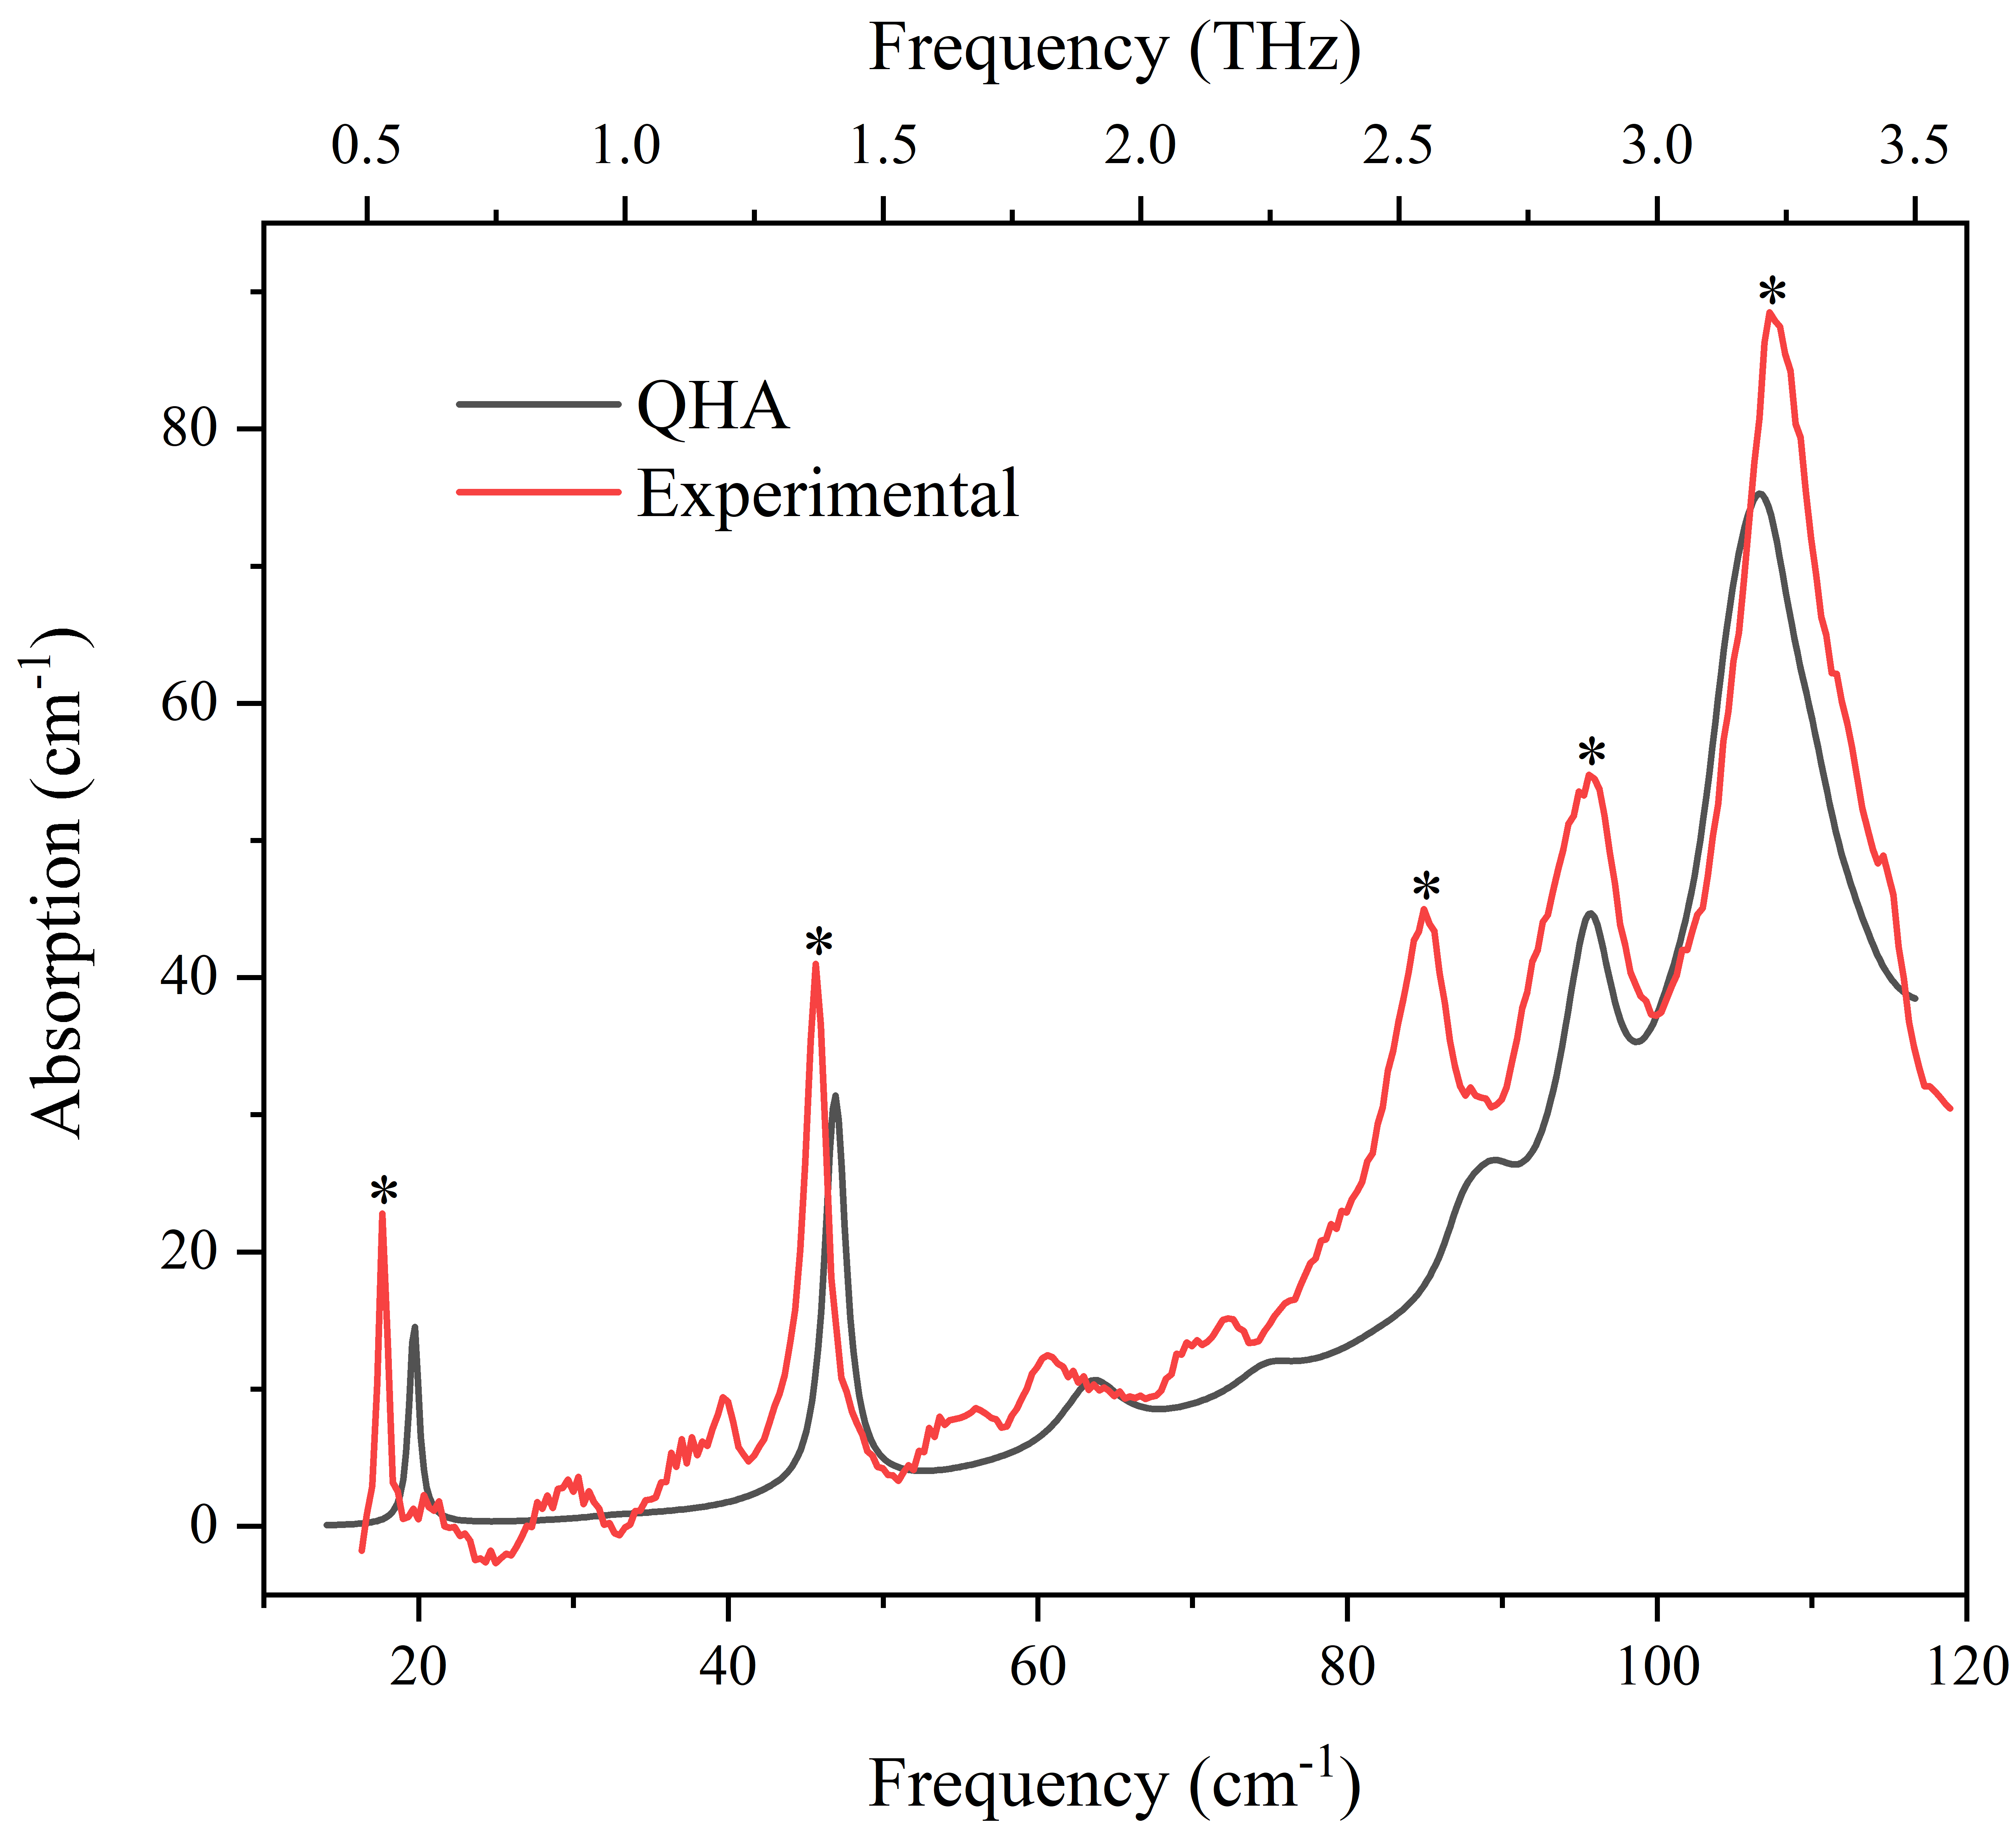
\includegraphics[width=\textwidth]{Figures/Spectra/RTEvsCG.png}
\caption{The experimental and calculated spectra at \SI{300}{K}}
\label{fig:RTvsEXP300K}
\end{subfigure}
\begin{subfigure}{0.49\textwidth}
\centering
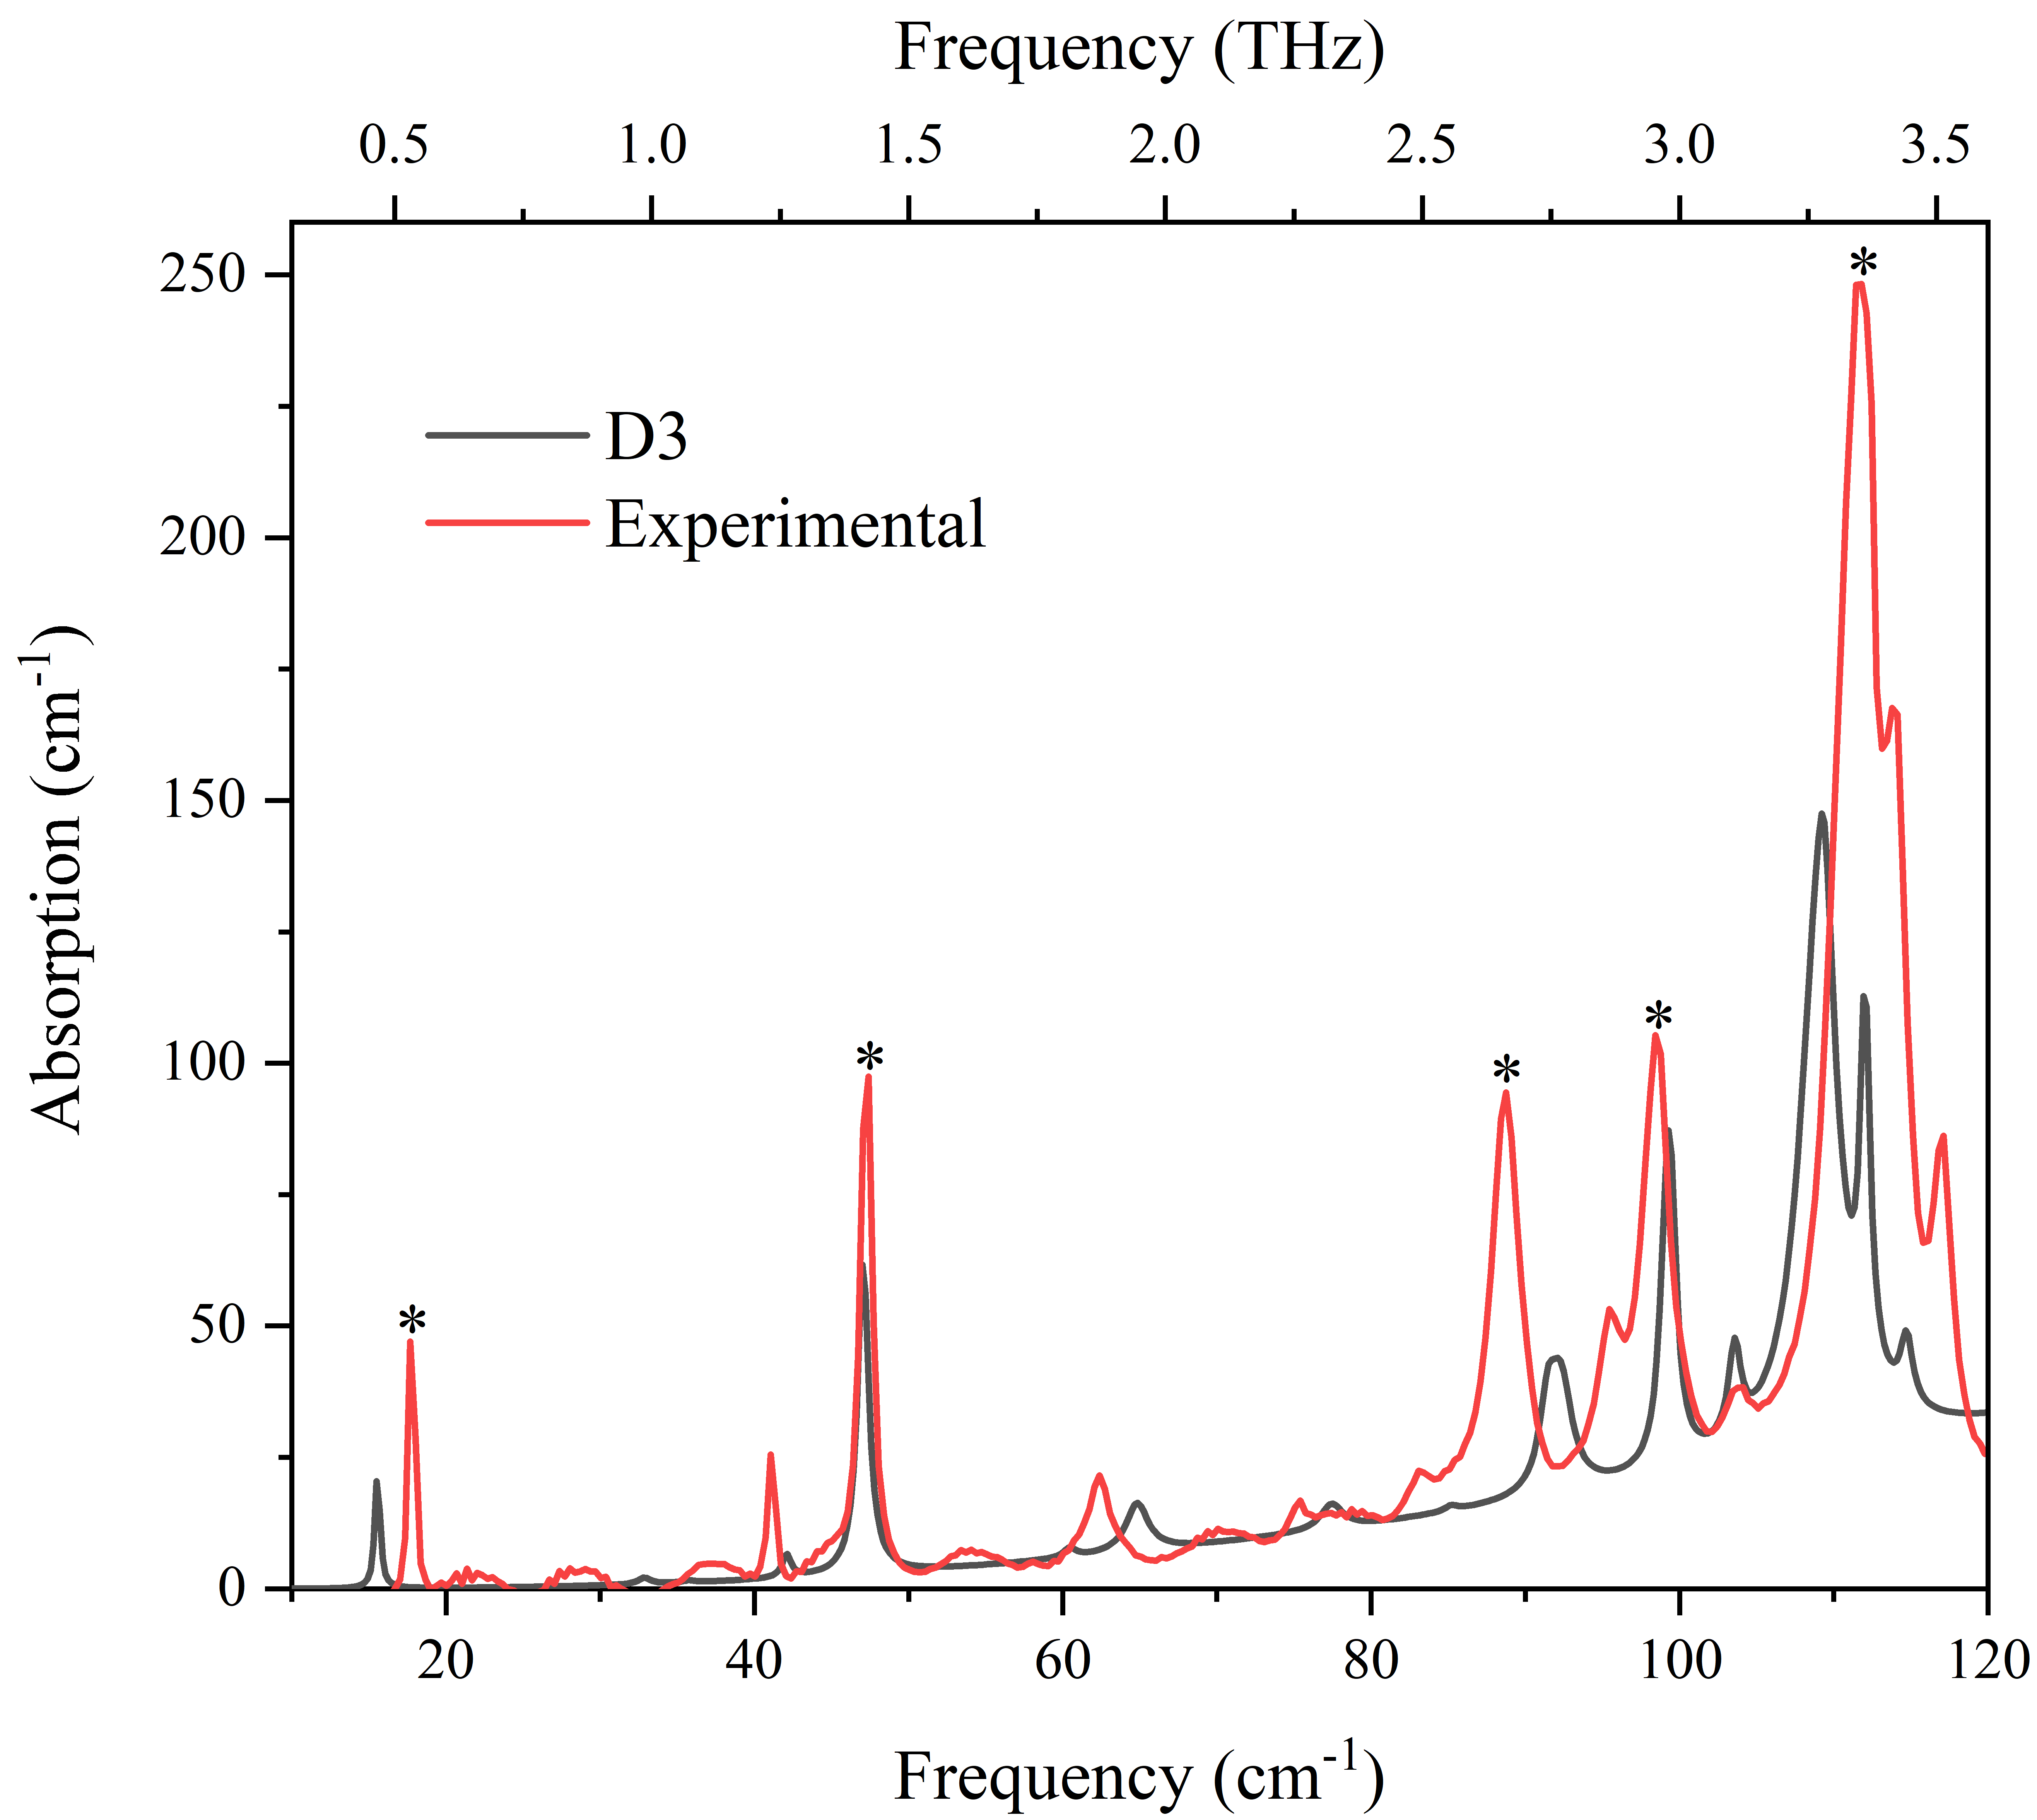
\includegraphics[width=\textwidth]{Figures/Spectra/D3ExpDiffG.png}
\caption{The experimental and calculated spectra at \SI{4}{K}}
\label{fig:RTvsEXP4K}
\end{subfigure}

\captionsetup{font = footnotesize, justification = centering}
\caption[The Calculated Terahertz Absorption Spectra at 300 and \SI{4}{K}]{The experimental and calculated terahertz absorption spectra at 300 and \SI{4}{K} respectively. The spectrum calculated at \SI{300}{K} shows greater correlation with experiment than the spectrum taken at \SI{4}{K} and the calculated intensities also show greater agreement.}
\label{Fig:RTvsEXP}
\end{figure}

The spectrum calculated at \SI{300}{K} shows excellent agreement with experiment, having an x-correlation value of 0.9416 and an \acrshort{rms} error of 0.0969 with a frequency shift of \SI{-0.2}{cm^{-1}} and a frequency scaling value of 0.95. This is significantly better than the spectrum calculated using the harmonic approximation when comparing to the spectrum measured at \SI{4}{K} which has an x\nobreakdash-correlation of 0.8749 and an \acrshort{rms} error of 0.106 in this frequency range. This is likely to be caused by the much finer detail within the \SI{4}{K} spectrum which would increase the complexity of exactly matching the experimental spectrum. Nearly all peaks show very good agreement across experiment and theory with the exception of the experimental peak at approximately \SI{85}{cm^{-1}}. This is the mode that also showed the most disagreement at \SI{4}{K} and the degree of mismatch has not increased. This means that what is causing the disagreement is either not affected by temperature or that the shift is consistent across experiment and calculation as temperature increases. The ratio of intensities between experiment and calculation is also better than for \SI{4}{K} which may be a result of the increased background absorption at higher temperatures.

One possible explanation of the large discrepancy between the calculated and experimental frequencies of Mode~3 is the impact this mode has on the surrounding structure. As shown in \Cref{fig:mode13_anharm}, Mode~3 consists of a number of \(O\)\nobreakdash--\(H\) groups oscillating close to each other. This is expected to drastically increase the change in total energy over the course of the oscillation when compared to, for example, Mode~1. This is shown in \Cref{fig:modemap}, where a method developed by Skelton \textit{et. al.} \cite{Skelton2016} allows for the mapping of the potential energy surface along a phonon coordinate and has been applied to Mode~1 and Mode~3. It is clear the potential for Mode~3 is much steeper than for Mode~1, which is expected to be the most harmonic mode, and this may result in the harmonic approximation being less appropriate for Mode~3 but being appropriate for Mode~1. Owing to time constraints, the other modes were not examined but this would aid in understanding whether the potentials of Mode~1 or Mode~3 are more common.

\begin{figure}[t]
\centering
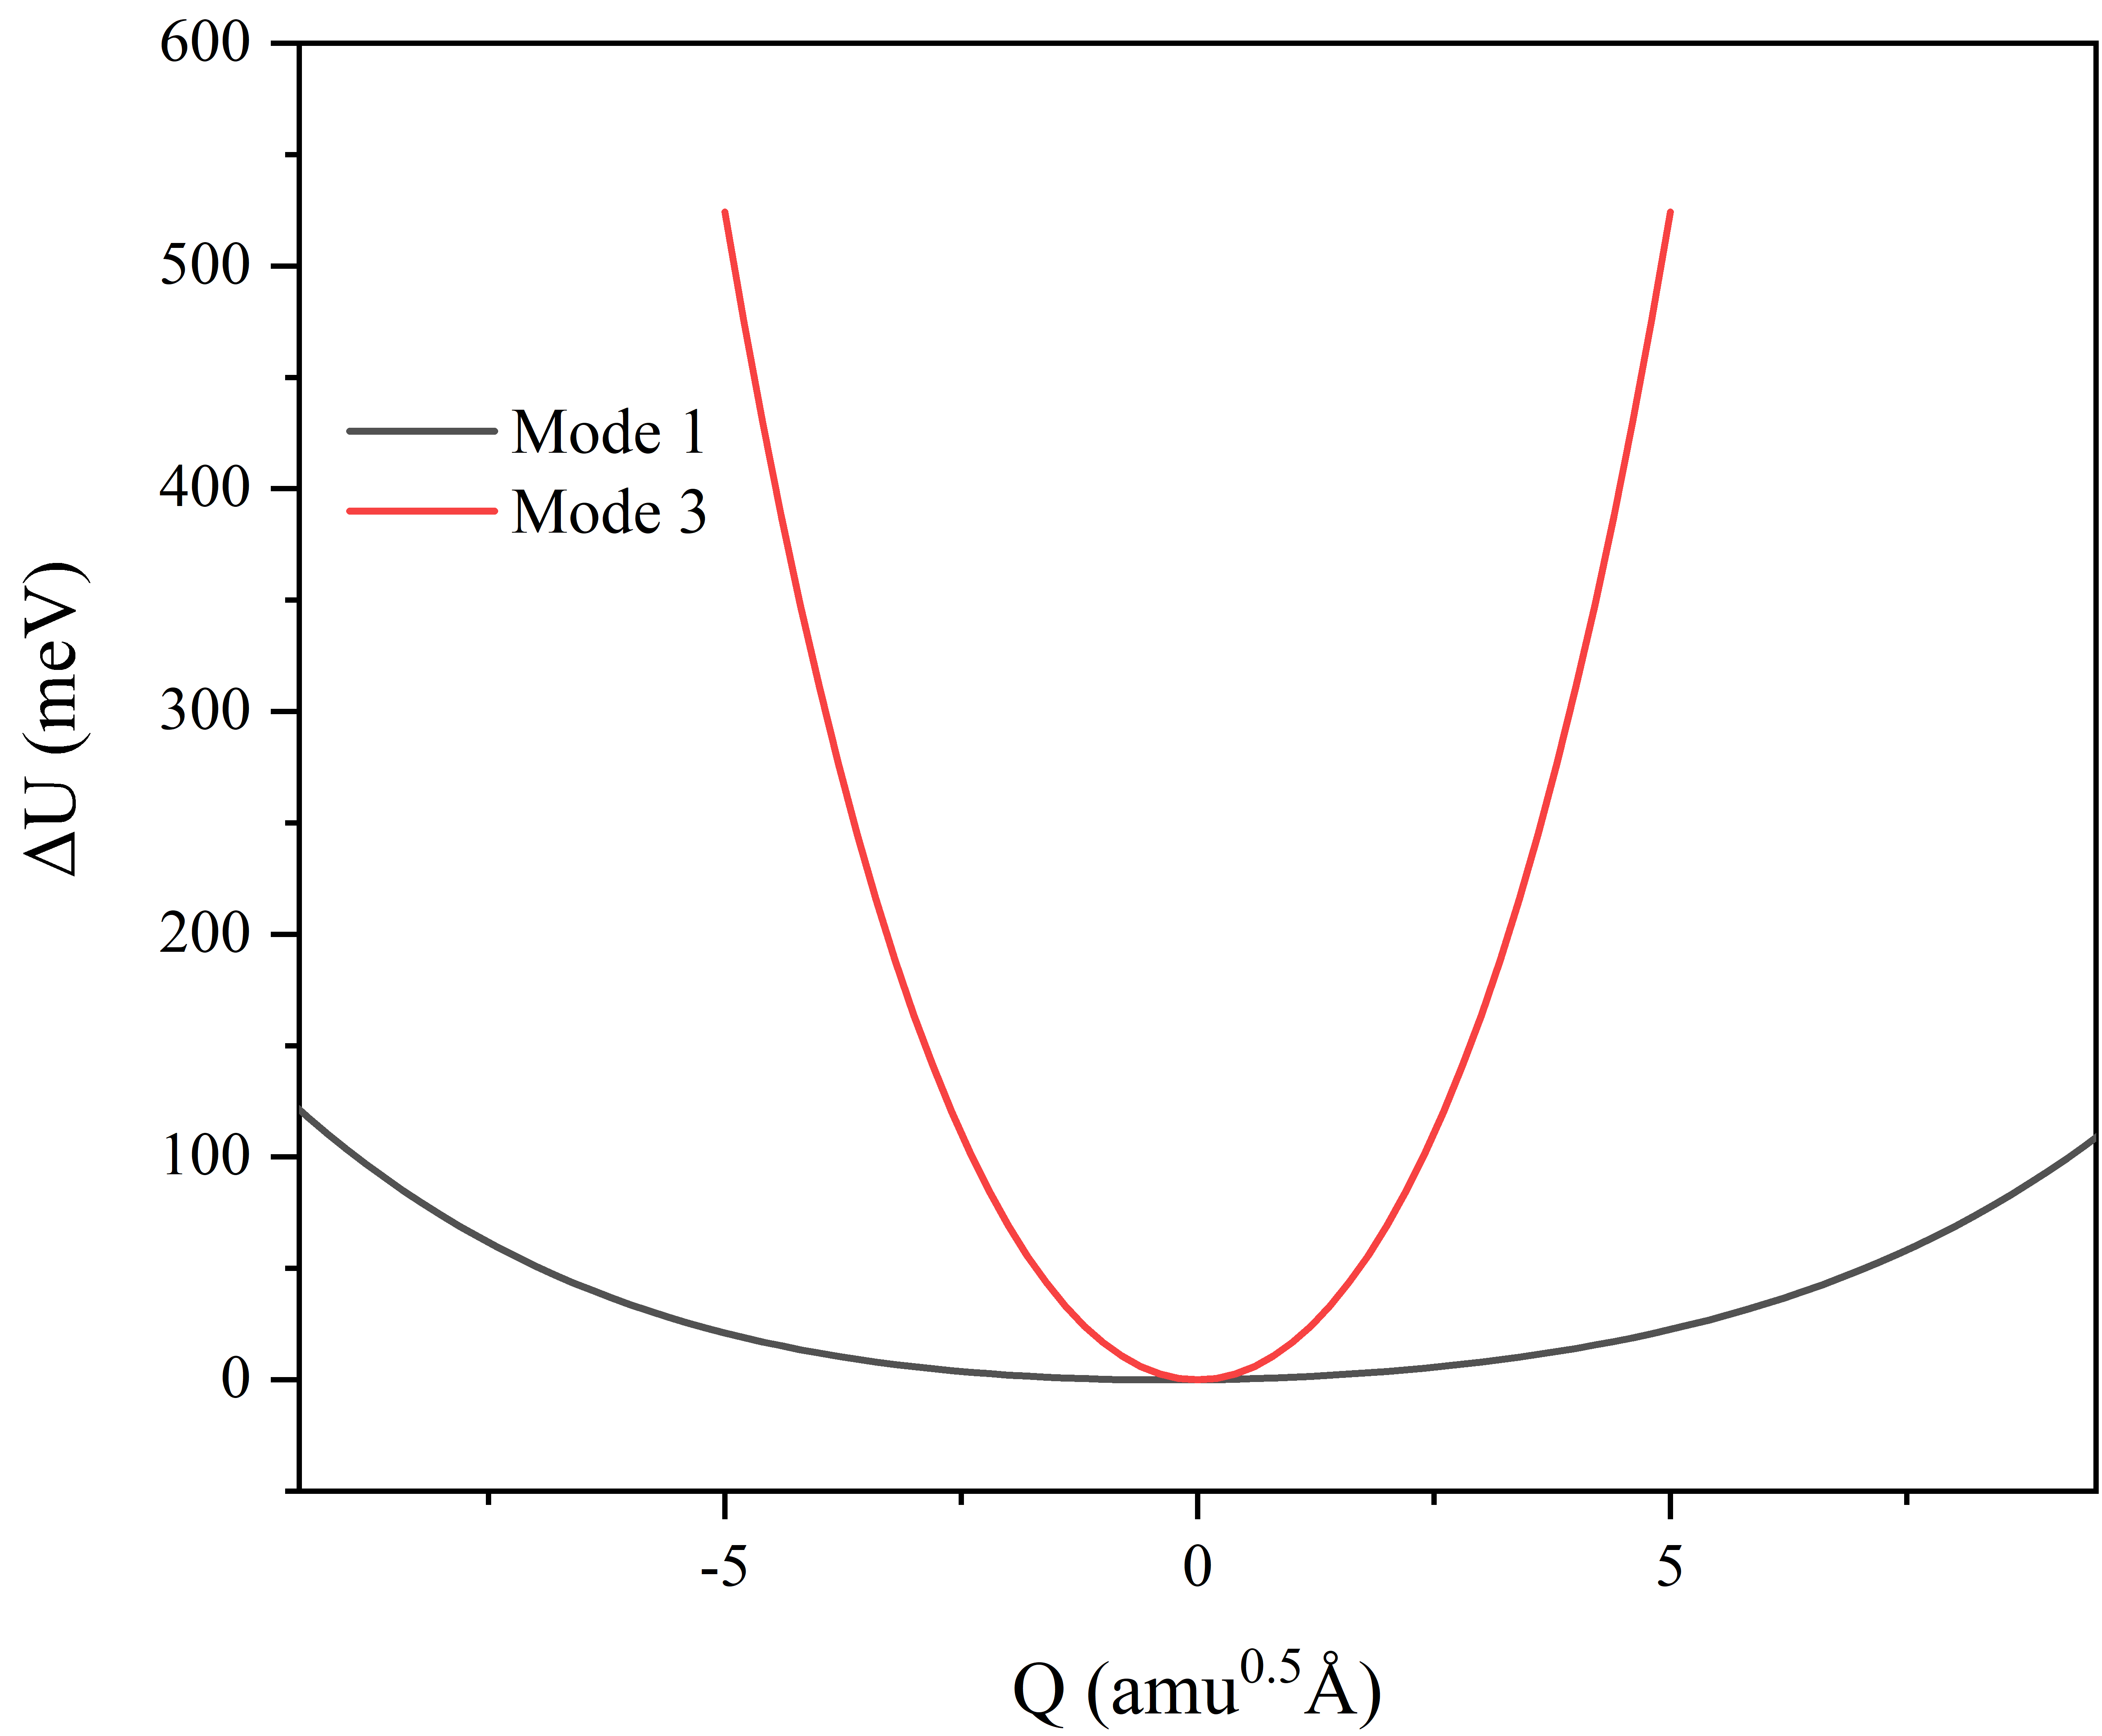
\includegraphics[scale=0.5]{Figures/Misc/QHA/ModeMapComparison.png}
\captionsetup{font = footnotesize, justification = centering}
\caption[The Change in the Potential Energy Surface as Mode~1 and Mode~3 are Projected along the Phonon Coordinates]{The change in the potential energy surface as Mode~1 and Mode~3 are projected along the phonon coordinates.}
\label{fig:modemap}
\end{figure}

\section{Conclusion}
In conclusion, the \acrshort{qha} approximation was used to calculate the thermodynamic properties and temperature\nobreakdash-dependent phonon frequencies of \acrshort{alm}. This was used to calculate the \acrshort{thz} absorption spectra at room temperature which had not previously been achieved by this group. Lastly, several modes and there trends with temperature were examined. This investigation produced both successes and failures, with the prediction of the unit cell volume at \SI{300}{K} being less than 1\% off the experimental value. The heat capacity of the system seemed to be drastically overestimated, being over by 78.9\% but this is not entirely unexpected for a system as large as \acrshort{alm}. However the production of the spectrum at room temperature can be considered a success owing to high degree of correlation with an experimental spectrum taken at room temperature. This should allow for simpler experimental setups that do not have to incorporate space for cryogenic apparatus and reduces the cost and risk of the measurement. However, at present this will be limited to systems where the number and environment of electrons is similar to \acrshort{alm} as the computational time to optimise and calculate phonon properties for all the volumes required is incredibly time\nobreakdash-consuming. Larger systems or systems involving large numbers of electrons, such as metals, could be analysed using this method but the required computational resources would be incredibly large. 
